\chapter{Detailed results}
\label{cha:detailed-results}
\section{Model 1}
\begin{tcolorbox}[
	breakable,
	arc=0mm,
	left=1pt,
	right = 1pt,
	boxrule=0mm,
	colback = {white},
	]
	\texttt{\input{./models/model1.txt}}
\end{tcolorbox}
\captionof{textdesc}{Text description for model 1}
\label{txt:model1}

{\scriptsize
	\begin{longtable}{|p{0.03 \hsize}|p{0.25 \hsize}|p{0.15 \hsize}|p{0.2 \hsize}|p{0.1 \hsize}|p{0.1 \hsize}|}
		\hline
		Order & Activity & Condition & Who & Subprocess & Terminated.
		\\\hline\hline
		\csvreader[late after line=\\\hline]
		{./results/model1_intermediate_model.csv}
		{Order=\Order,Activity=\Activity,Condition=\Condition,Who=\Who,Subprocess=\Subprocess,Terminated=\Terminated}
		{\Order & \Activity & \Condition & \Who & \Subprocess & \Terminated}
		\caption{Spreadsheet-based description for process model 1}
		\label{csv:model1}
	\end{longtable}
}

\begin{figure}[H]
	\centering
	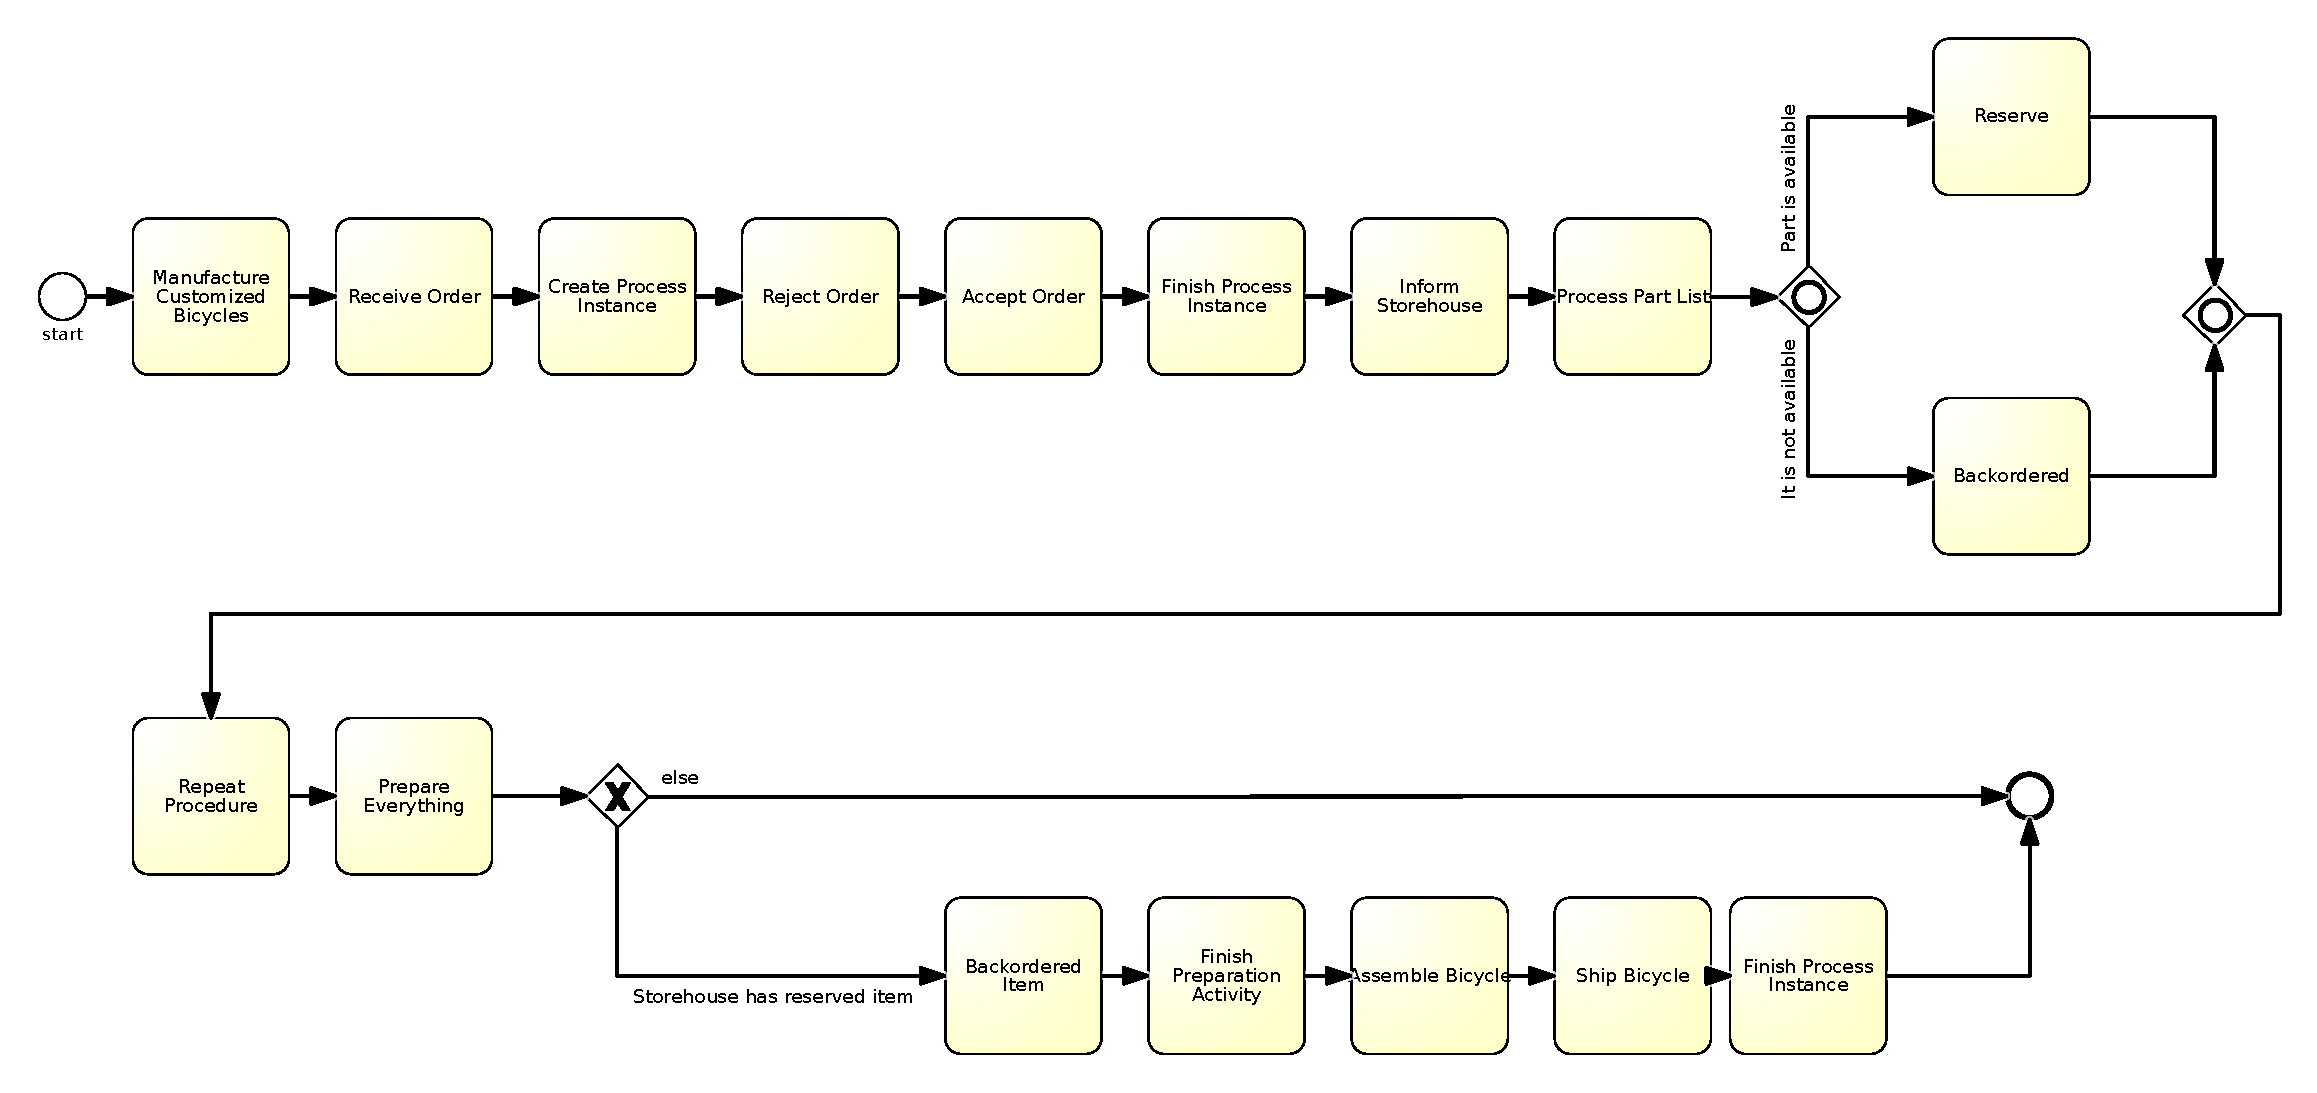
\includegraphics[width=\hsize]{./generated_bpmn/model1.pdf}
	\caption{BPMN diagram for process model 1 generated from spreadsheet-based model}
	\label{bpmn:generated_model1}
\end{figure}

\begin{figure}[H]
	\centering
	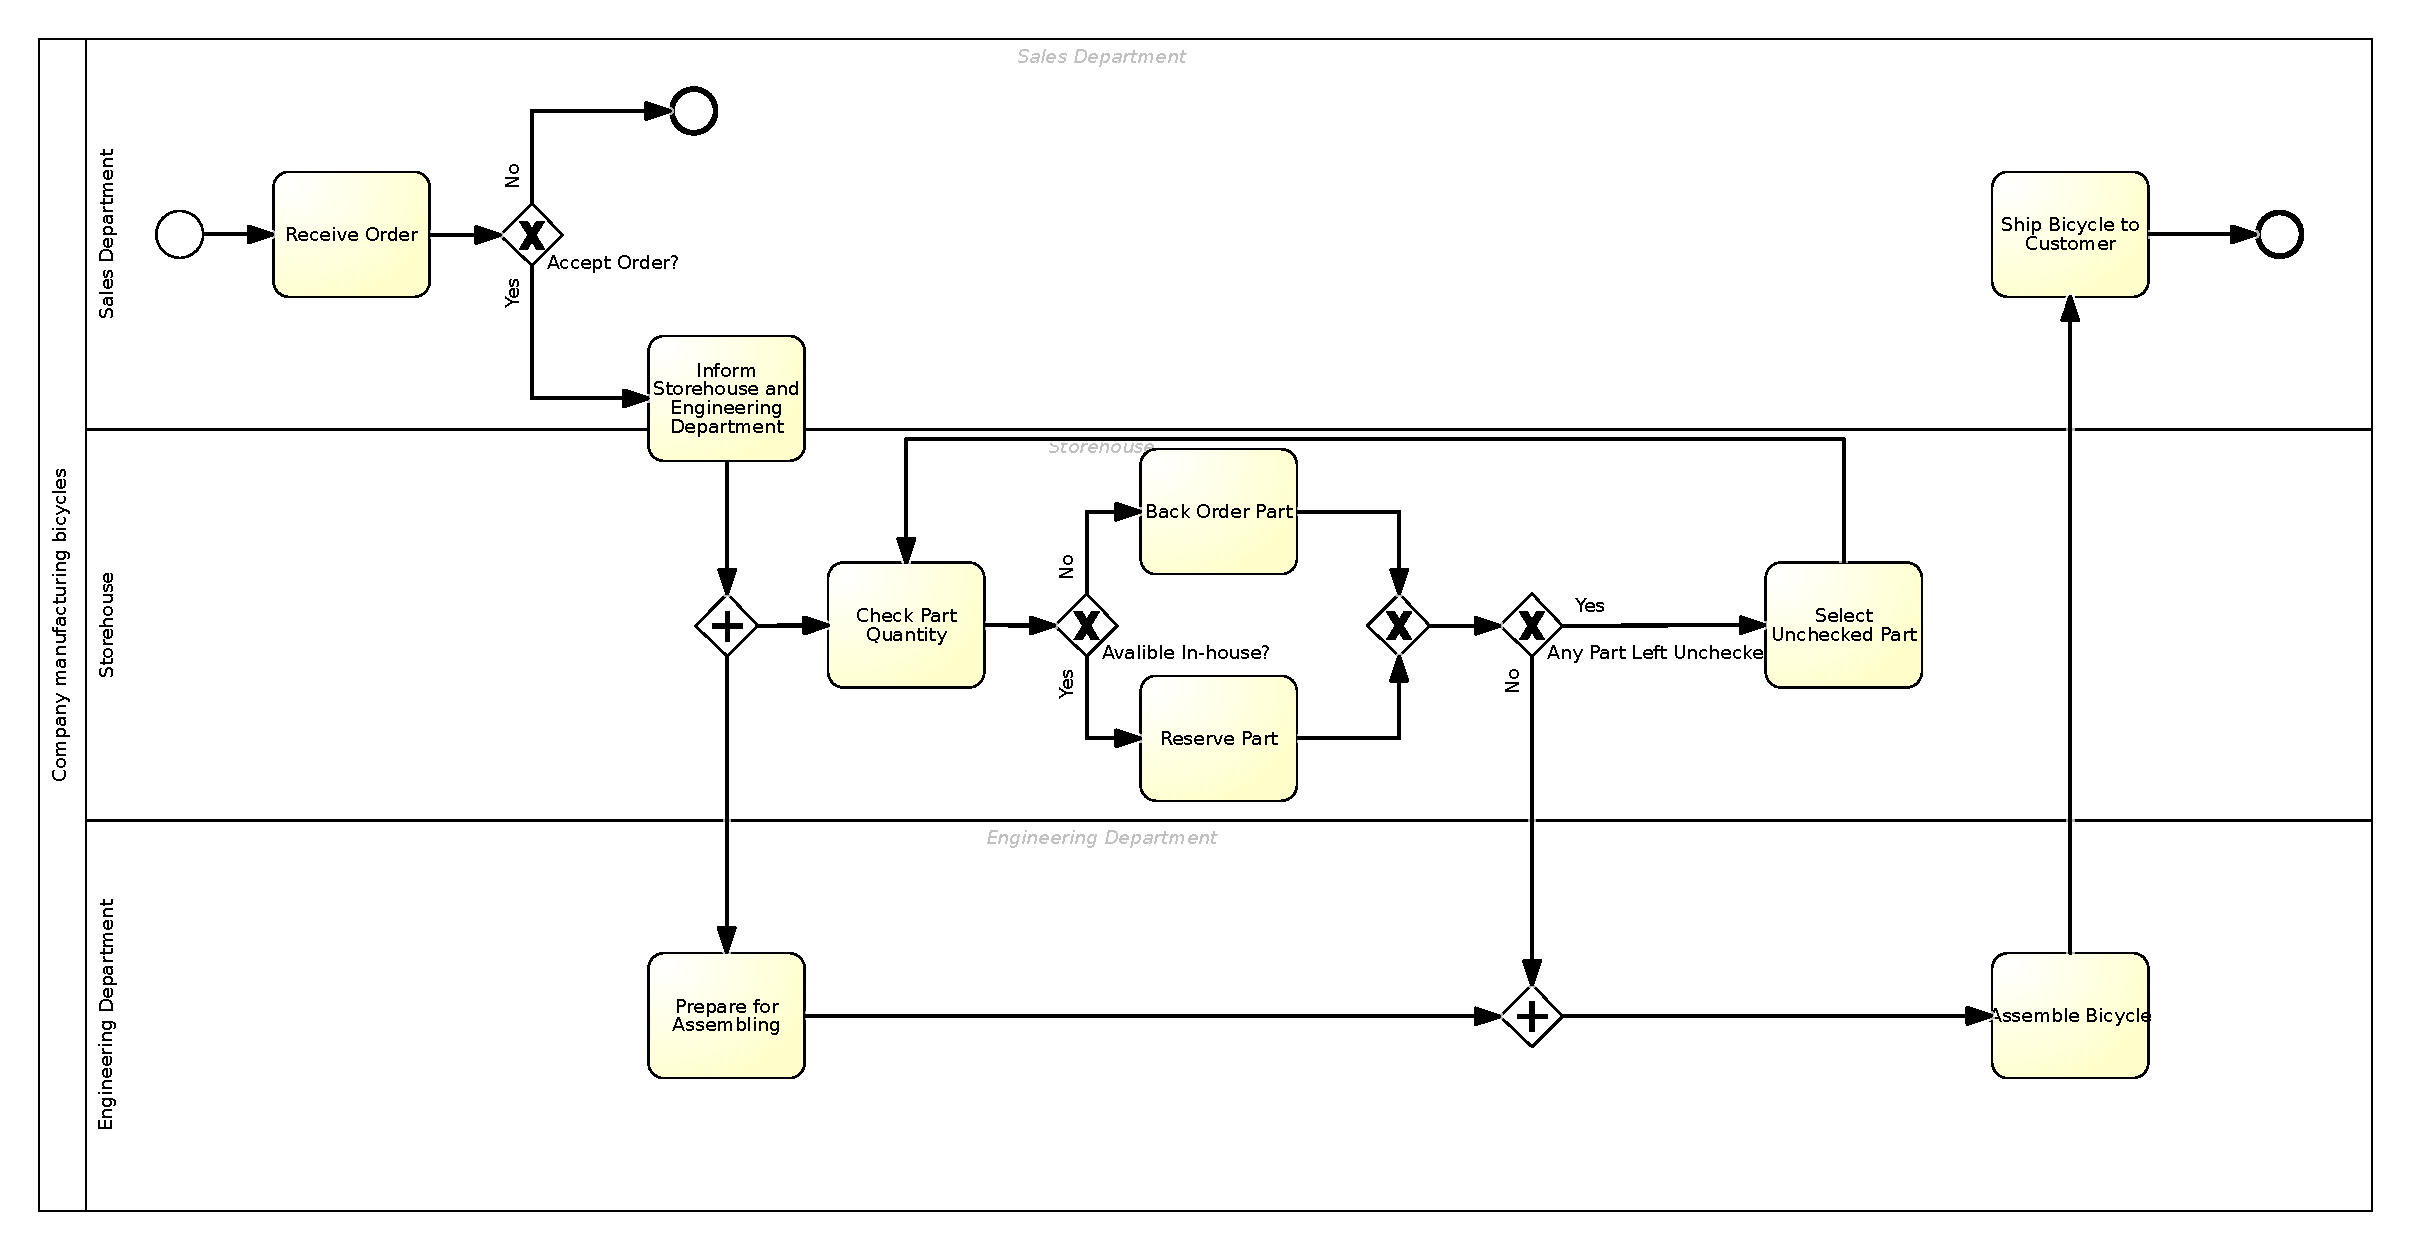
\includegraphics[width=\hsize]{./bpmn/model1.pdf}
	\caption{Hand-made BPMN diagram for process model 1}
	\label{bpmn:model1}
\end{figure}

\section{Model 2}
\begin{tcolorbox}[
	breakable,
	arc=0mm,
	left=1pt,
	right = 1pt,
	boxrule=0mm,
	colback = {white},
	]
	\texttt{\input{./models/model2.txt}}
\end{tcolorbox}
\captionof{textdesc}{Text description for model 2}
\label{txt:model2}

{\scriptsize
	\begin{longtable}{|p{0.03 \hsize}|p{0.25 \hsize}|p{0.15 \hsize}|p{0.2 \hsize}|p{0.1 \hsize}|p{0.1 \hsize}|}
		\hline
		Order & Activity & Condition & Who & Subprocess & Terminated.
		\\\hline\hline
		\csvreader[late after line=\\\hline]
		{./results/model2_intermediate_model.csv}
		{Order=\Order,Activity=\Activity,Condition=\Condition,Who=\Who,Subprocess=\Subprocess,Terminated=\Terminated}
		{\Order & \Activity & \Condition & \Who & \Subprocess & \Terminated}
		\caption{Spreadsheet-based description for process model 2}
		\label{csv:model2}
	\end{longtable}
}

\begin{figure}[H]
	\centering
	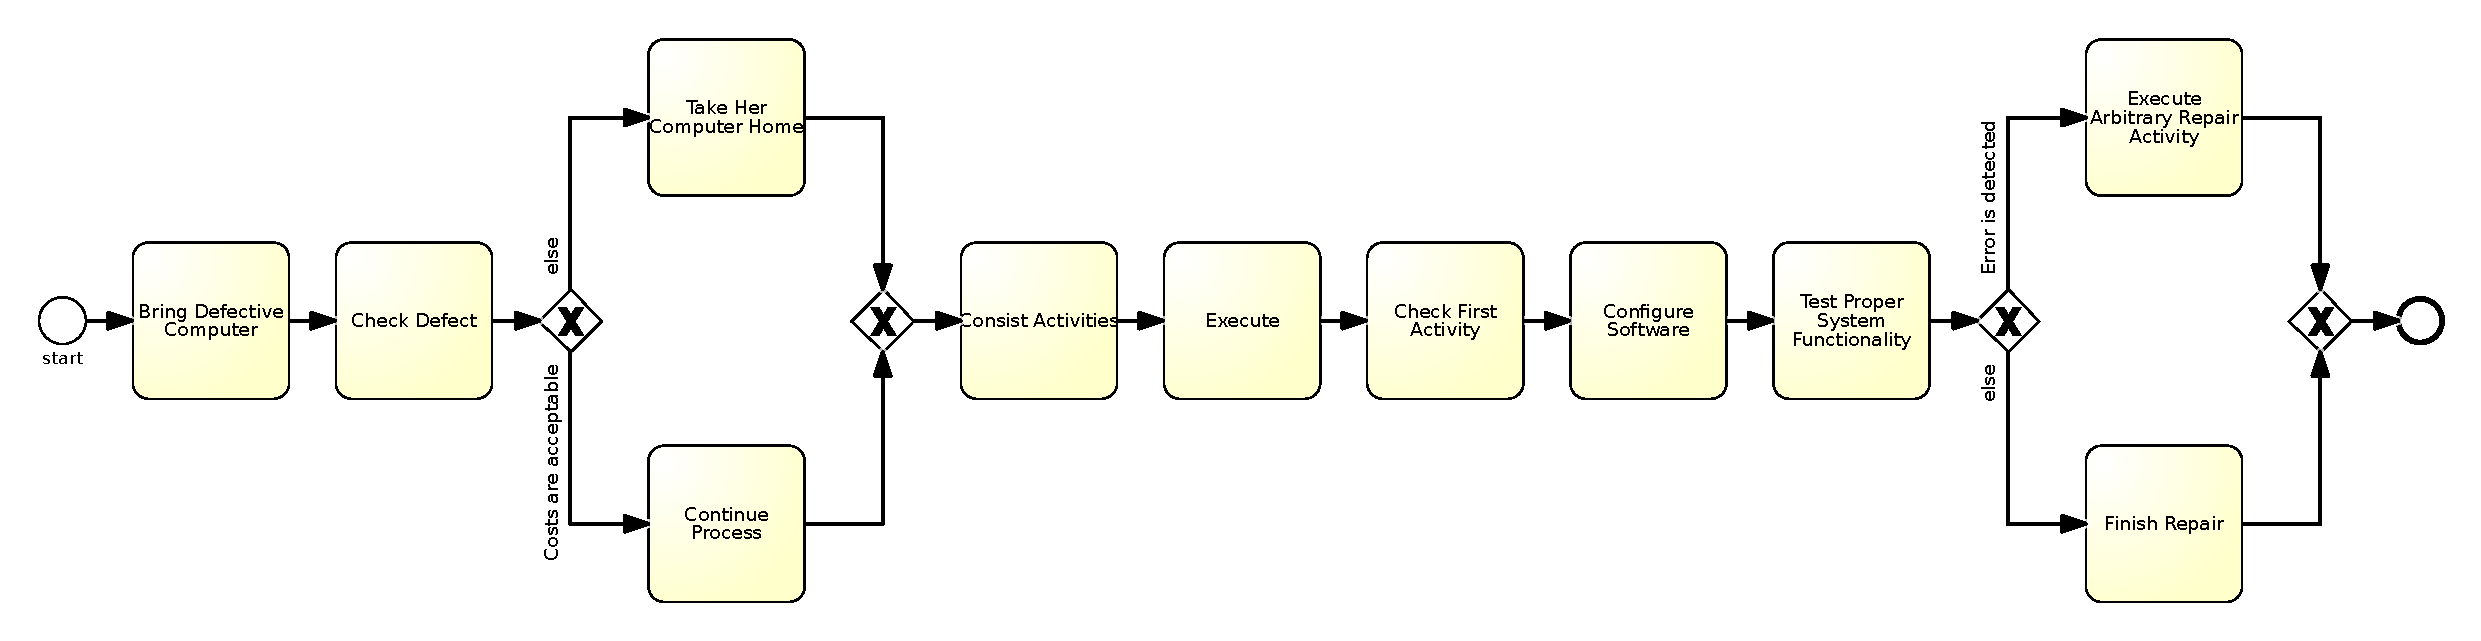
\includegraphics[width=\hsize]{./generated_bpmn/model2.pdf}
	\caption{BPMN diagram for process model 2 generated from spreadsheet-based model}
	\label{bpmn:generated_model2}
\end{figure}

\begin{figure}[H]
	\centering
	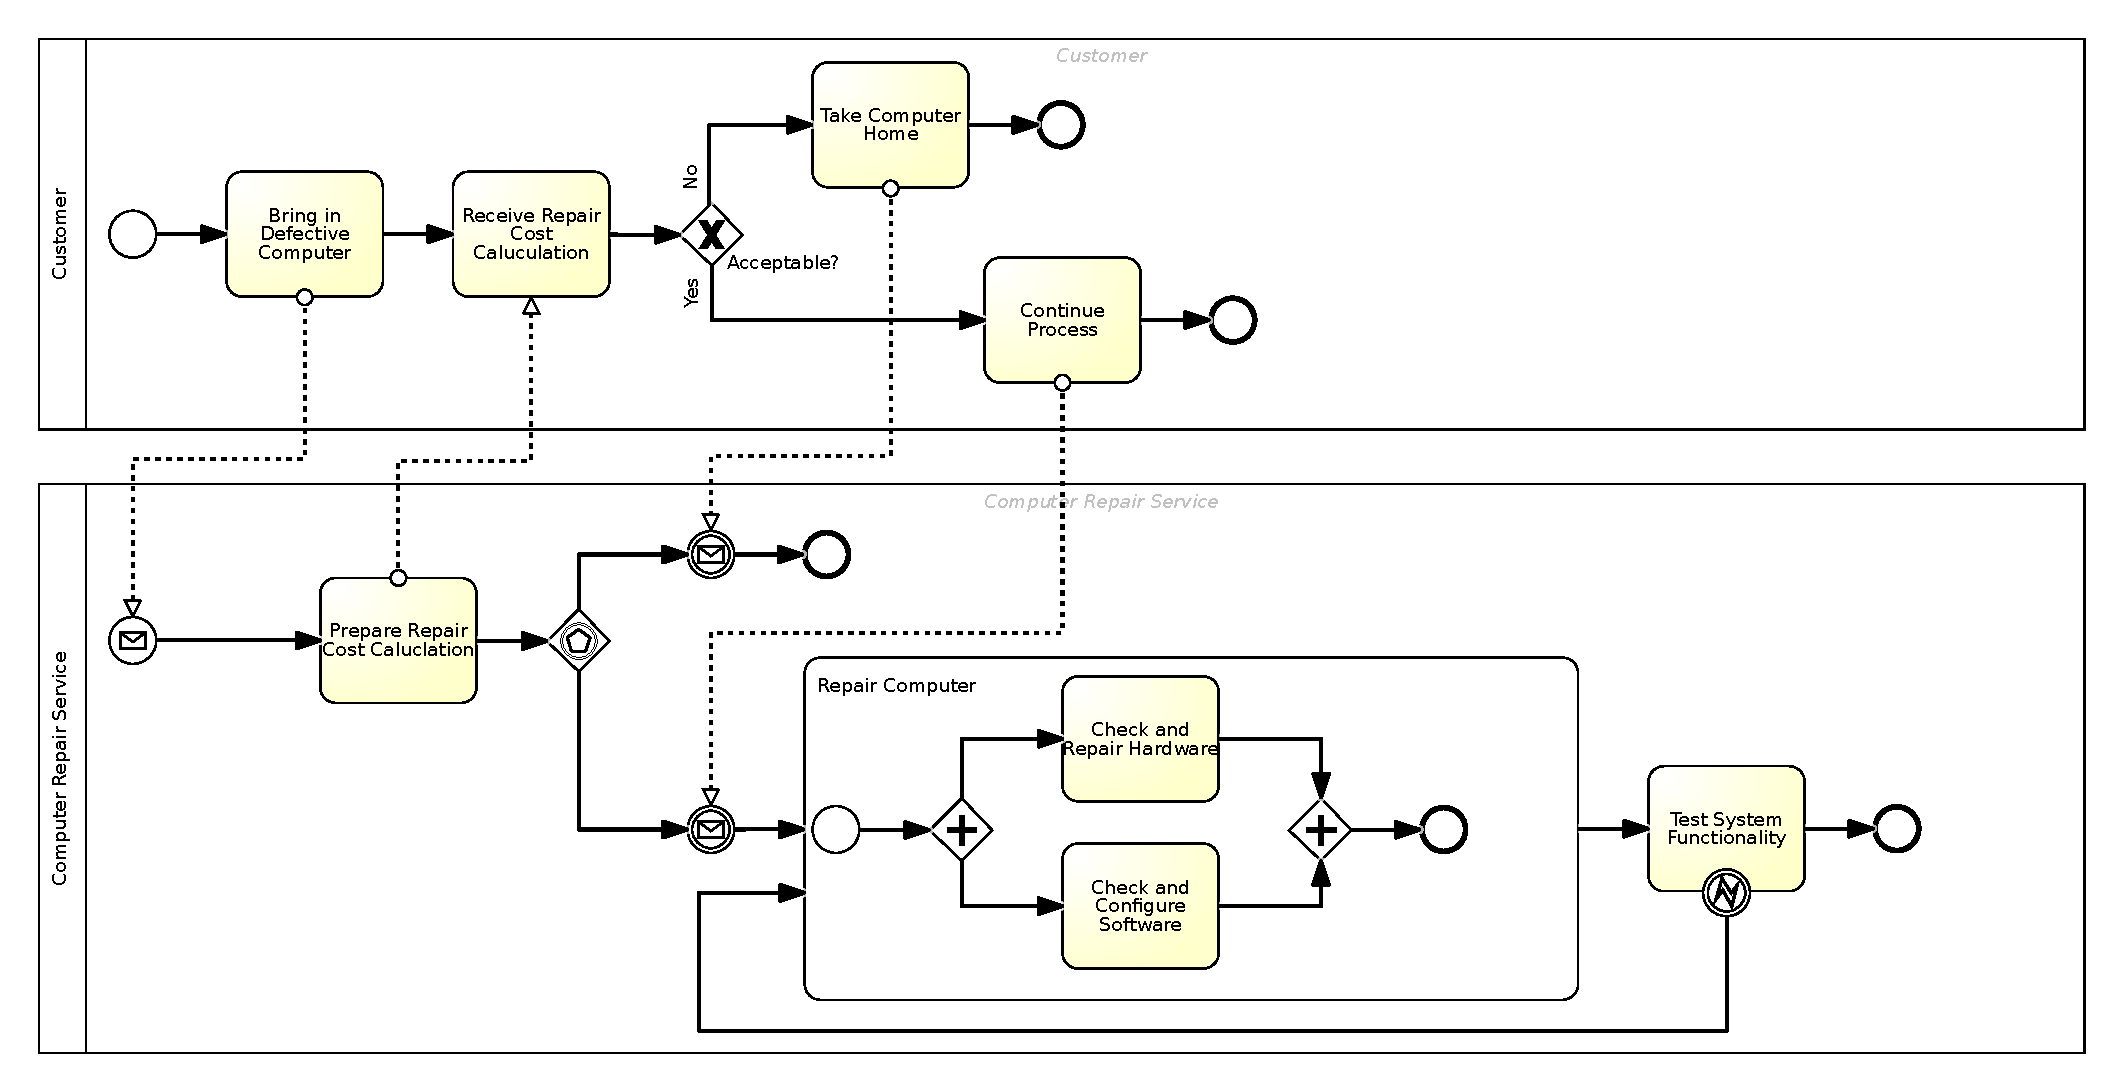
\includegraphics[width=\hsize]{./bpmn/model2.pdf}
	\caption{Hand-made BPMN diagram for process model 2}
	\label{bpmn:model2}
\end{figure}

\section{Model 3}
\begin{tcolorbox}[
	breakable,
	arc=0mm,
	left=1pt,
	right = 1pt,
	boxrule=0mm,
	colback = {white},
	]
	\texttt{\input{./models/model3.txt}}
\end{tcolorbox}
\captionof{textdesc}{Text description for model 3}
\label{txt:model3}

{\scriptsize
	\begin{longtable}{|p{0.03 \hsize}|p{0.25 \hsize}|p{0.15 \hsize}|p{0.2 \hsize}|p{0.1 \hsize}|p{0.1 \hsize}|}
		\hline
		Order & Activity & Condition & Who & Subprocess & Terminated.
		\\\hline\hline
		\csvreader[late after line=\\\hline]
		{./results/model3_intermediate_model.csv}
		{Order=\Order,Activity=\Activity,Condition=\Condition,Who=\Who,Subprocess=\Subprocess,Terminated=\Terminated}
		{\Order & \Activity & \Condition & \Who & \Subprocess & \Terminated}
		\caption{Spreadsheet-based description for process model 3}
		\label{csv:model3}
	\end{longtable}
}

\begin{figure}[H]
	\centering
	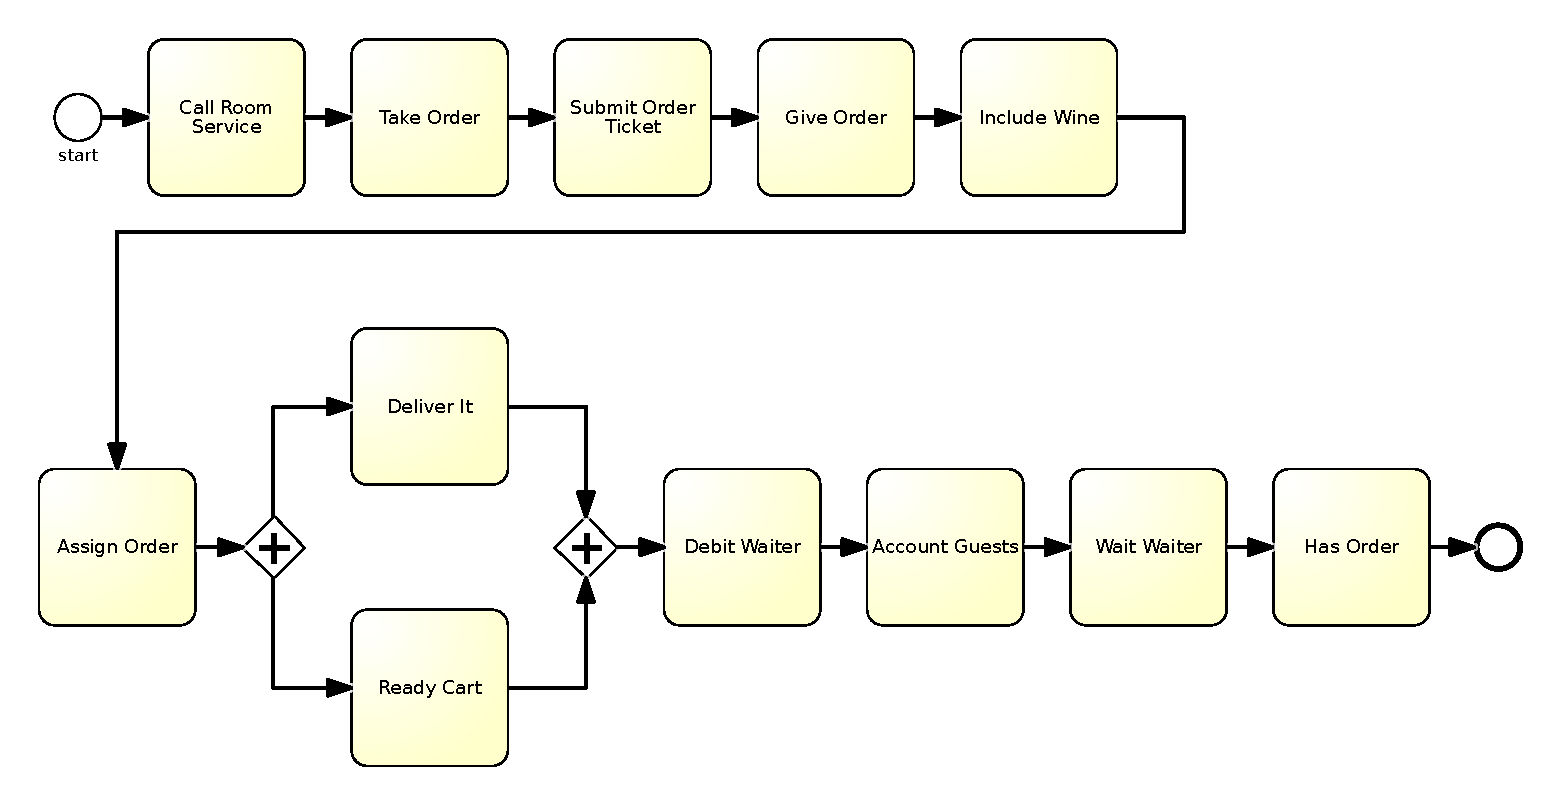
\includegraphics[width=\hsize]{./generated_bpmn/model3.pdf}
	\caption{BPMN diagram for process model 3 generated from spreadsheet-based model}
	\label{bpmn:generated_model3}
\end{figure}

\begin{figure}[H]
	\centering
	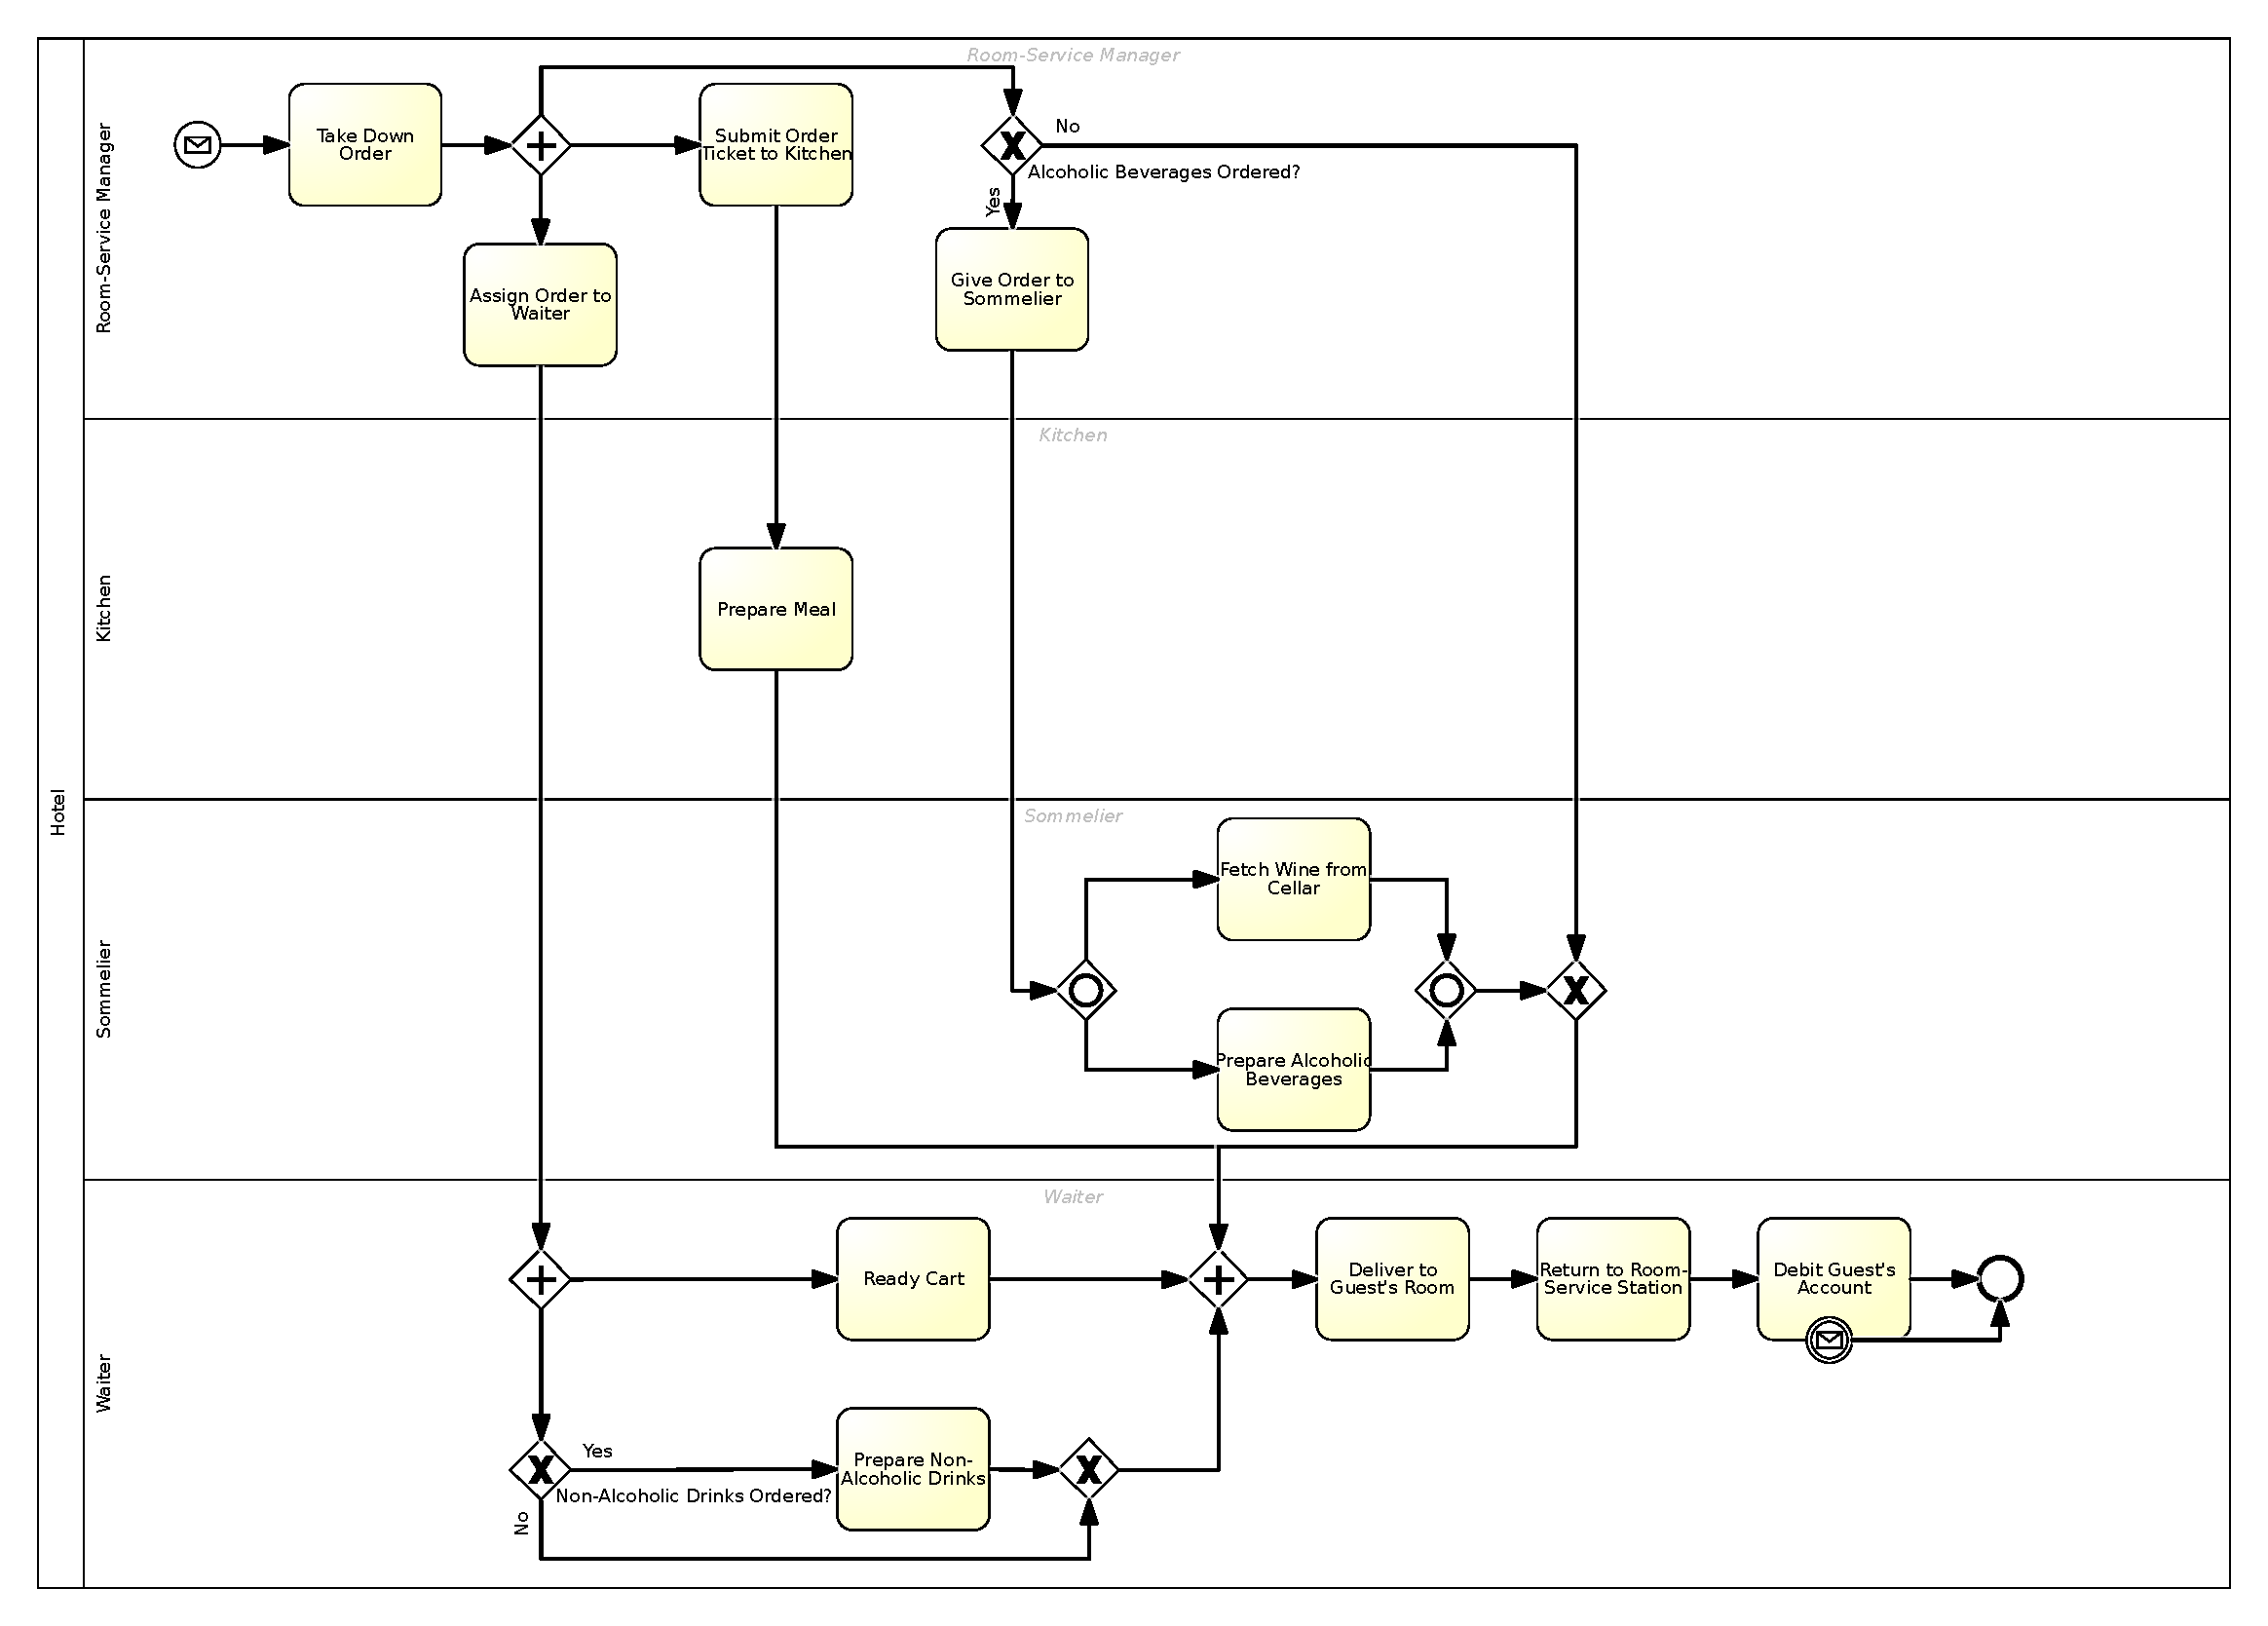
\includegraphics[width=\hsize]{./bpmn/model3.pdf}
	\caption{Hand-made BPMN diagram for process model 3}
	\label{bpmn:model3}
\end{figure}

\section{Model 4}
\begin{tcolorbox}[
	breakable,
	arc=0mm,
	left=1pt,
	right = 1pt,
	boxrule=0mm,
	colback = {white},
	]
	\texttt{\input{./models/model4.txt}}
\end{tcolorbox}
\captionof{textdesc}{Text description for model 4}
\label{txt:model4}

{\scriptsize
	\begin{longtable}{|p{0.03 \hsize}|p{0.25 \hsize}|p{0.15 \hsize}|p{0.2 \hsize}|p{0.1 \hsize}|p{0.1 \hsize}|}
		\hline
		Order & Activity & Condition & Who & Subprocess & Terminated.
		\\\hline\hline
		\csvreader[late after line=\\\hline]
		{./results/model4_intermediate_model.csv}
		{Order=\Order,Activity=\Activity,Condition=\Condition,Who=\Who,Subprocess=\Subprocess,Terminated=\Terminated}
		{\Order & \Activity & \Condition & \Who & \Subprocess & \Terminated}
		\caption{Spreadsheet-based description for process model 4}
		\label{csv:model4}
	\end{longtable}
}

\begin{figure}[H]
	\centering
	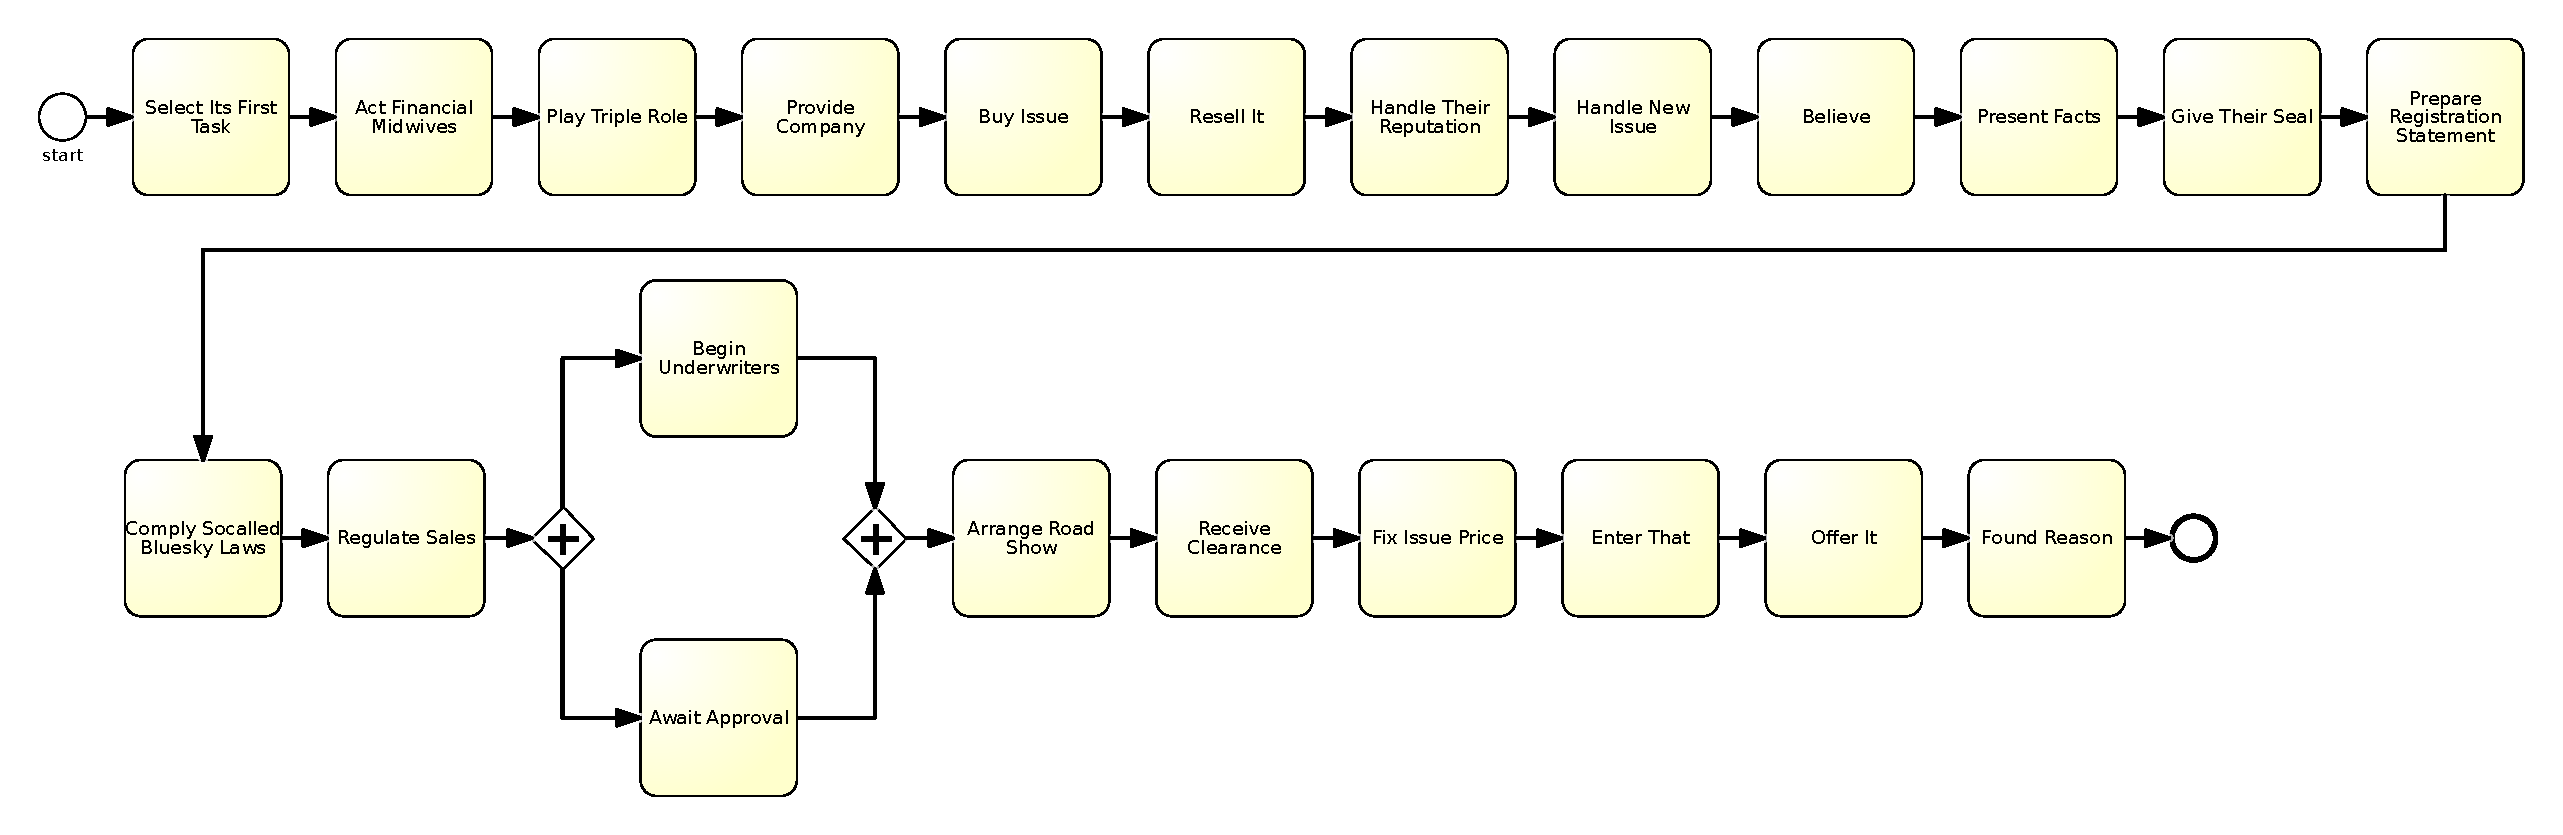
\includegraphics[scale=0.35]{./generated_bpmn/model4.pdf}
	\caption{BPMN diagram for process model 4 generated from spreadsheet-based model}
	\label{bpmn:generated_model4}
\end{figure}

\begin{figure}[H]
	\centering
	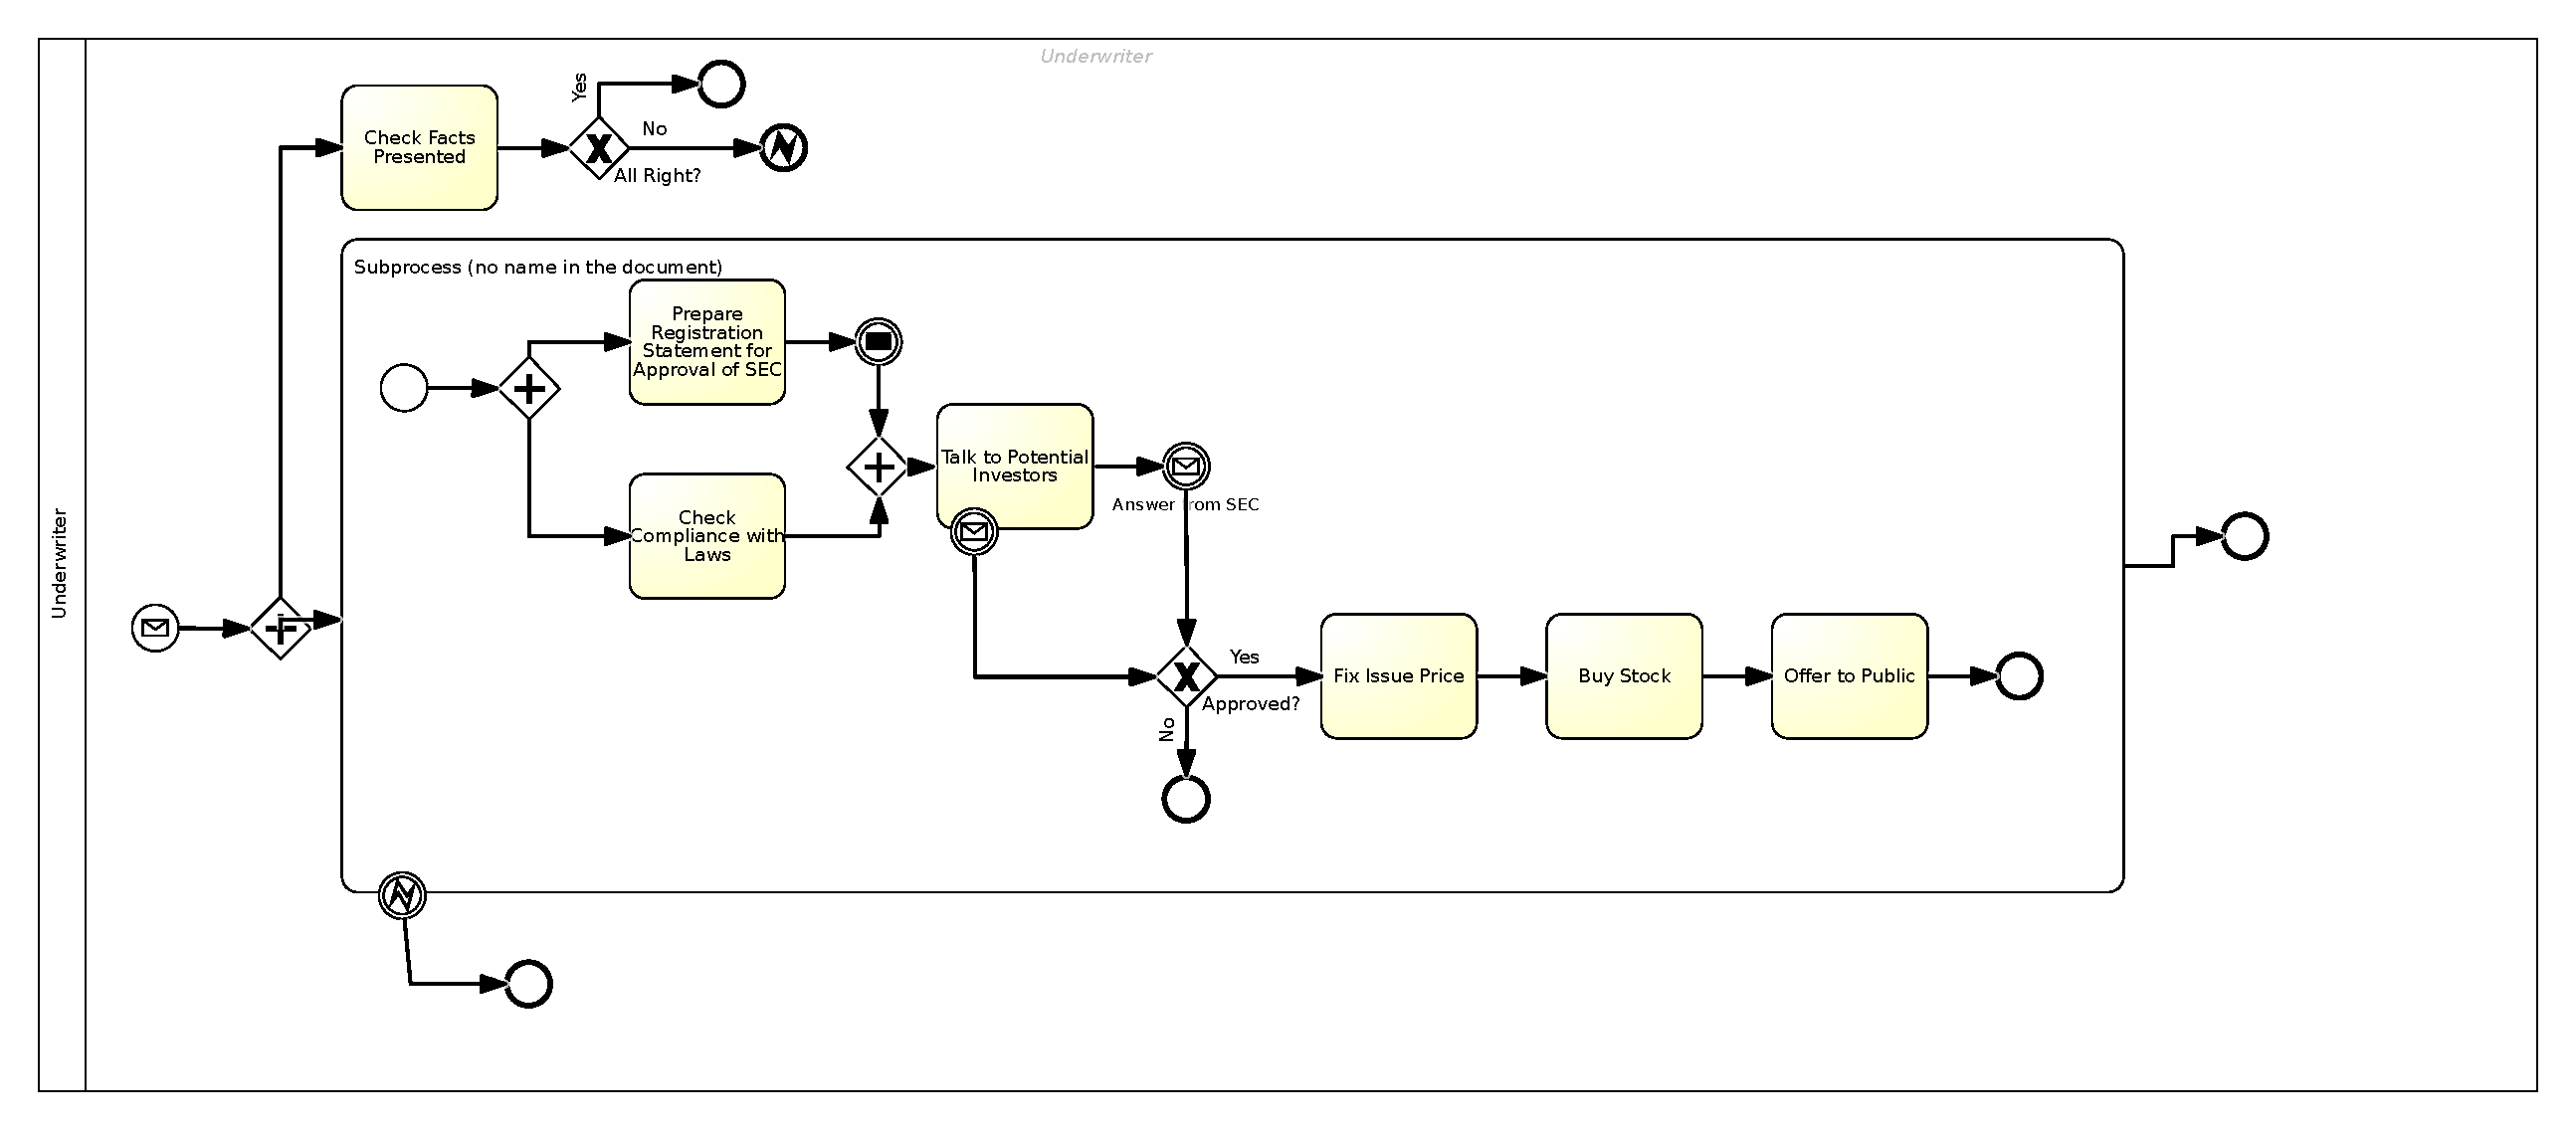
\includegraphics[width=\hsize]{./bpmn/model4.pdf}
	\caption{Hand-made BPMN diagram for process model 4}
	\label{bpmn:model4}
\end{figure}

\section{Model 5}
\begin{tcolorbox}[
	breakable,
	arc=0mm,
	left=1pt,
	right = 1pt,
	boxrule=0mm,
	colback = {white},
	]
	\texttt{\input{./models/model5.txt}}
\end{tcolorbox}
\captionof{textdesc}{Text description for model 5}
\label{txt:model5}

{\scriptsize
	\begin{longtable}{|p{0.03 \hsize}|p{0.25 \hsize}|p{0.15 \hsize}|p{0.2 \hsize}|p{0.1 \hsize}|p{0.1 \hsize}|}
		\hline
		Order & Activity & Condition & Who & Subprocess & Terminated.
		\\\hline\hline
		\csvreader[late after line=\\\hline]
		{./results/model5_intermediate_model.csv}
		{Order=\Order,Activity=\Activity,Condition=\Condition,Who=\Who,Subprocess=\Subprocess,Terminated=\Terminated}
		{\Order & \Activity & \Condition & \Who & \Subprocess & \Terminated}
		\caption{Spreadsheet-based description for process model 5}
		\label{csv:model5}
	\end{longtable}
}

\begin{figure}[H]
	\centering
	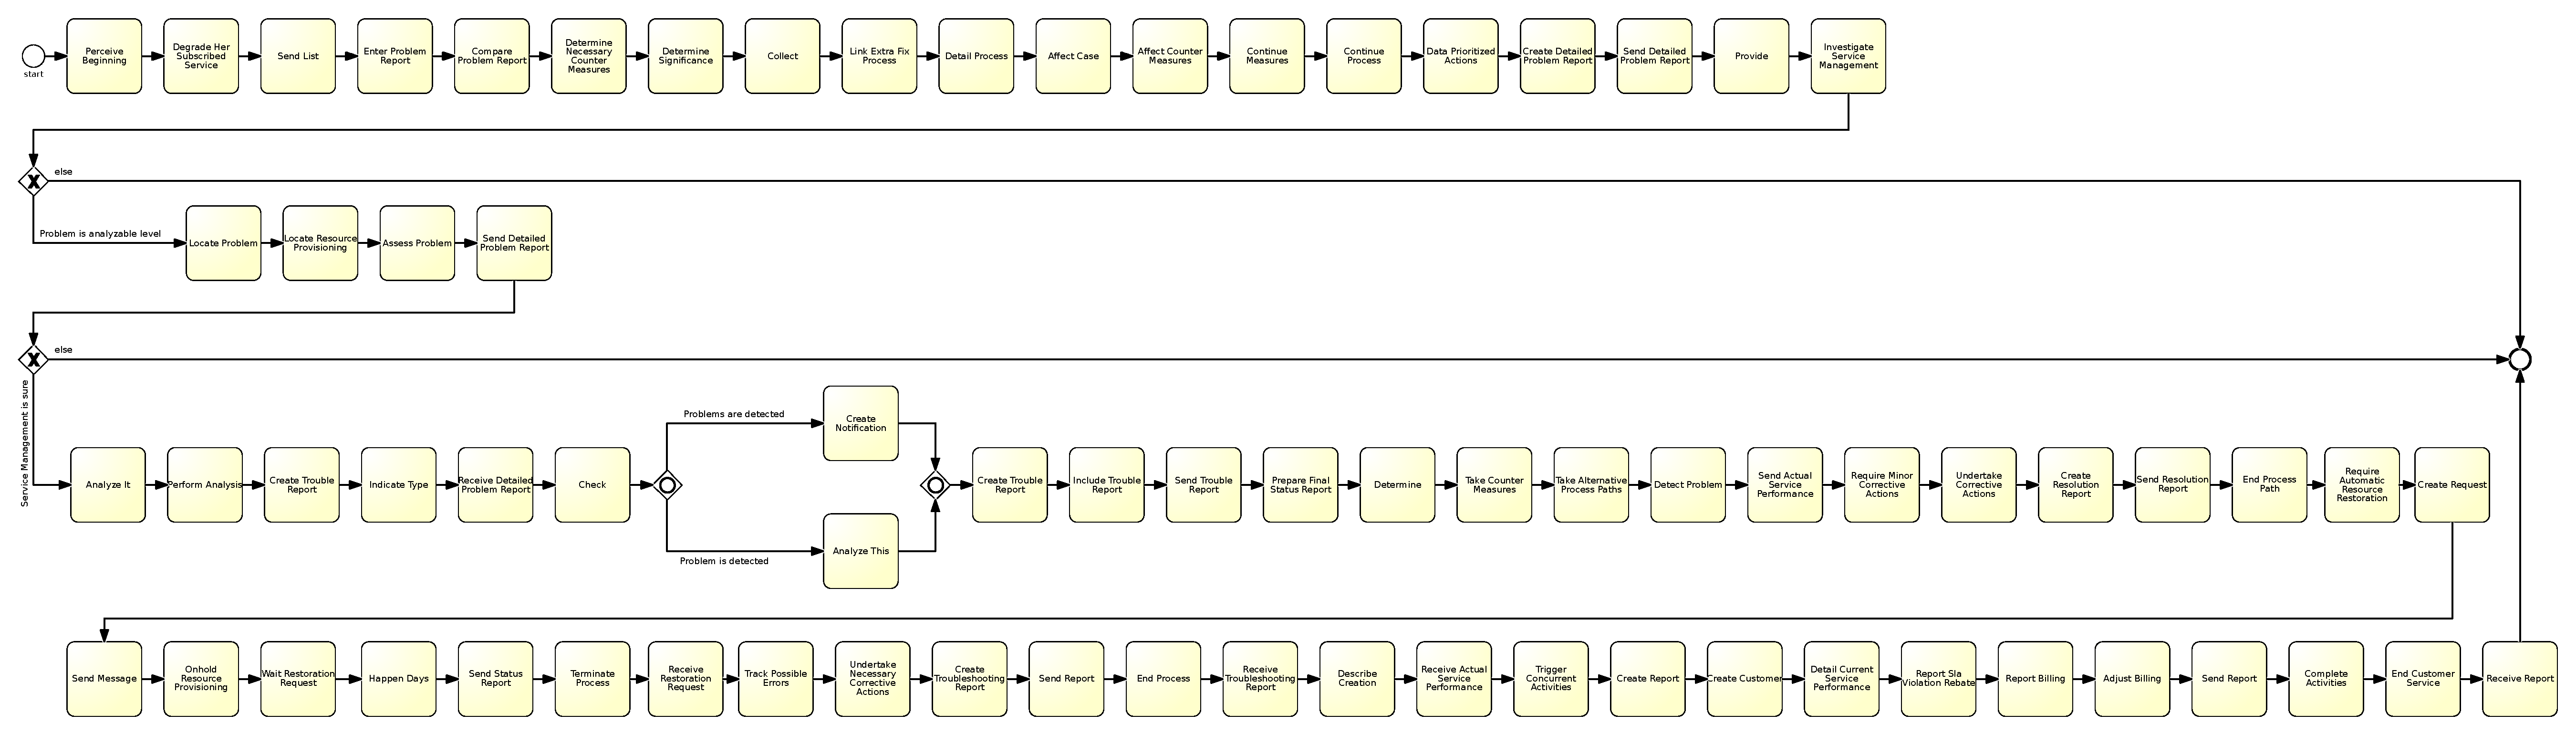
\includegraphics[width=0.95\textheight, angle=90]{./generated_bpmn/model5.pdf}
	\caption{BPMN diagram for process model 5 generated from spreadsheet-based model}
	\label{bpmn:generated_model5}
\end{figure}

\begin{figure}[H]
	\centering
	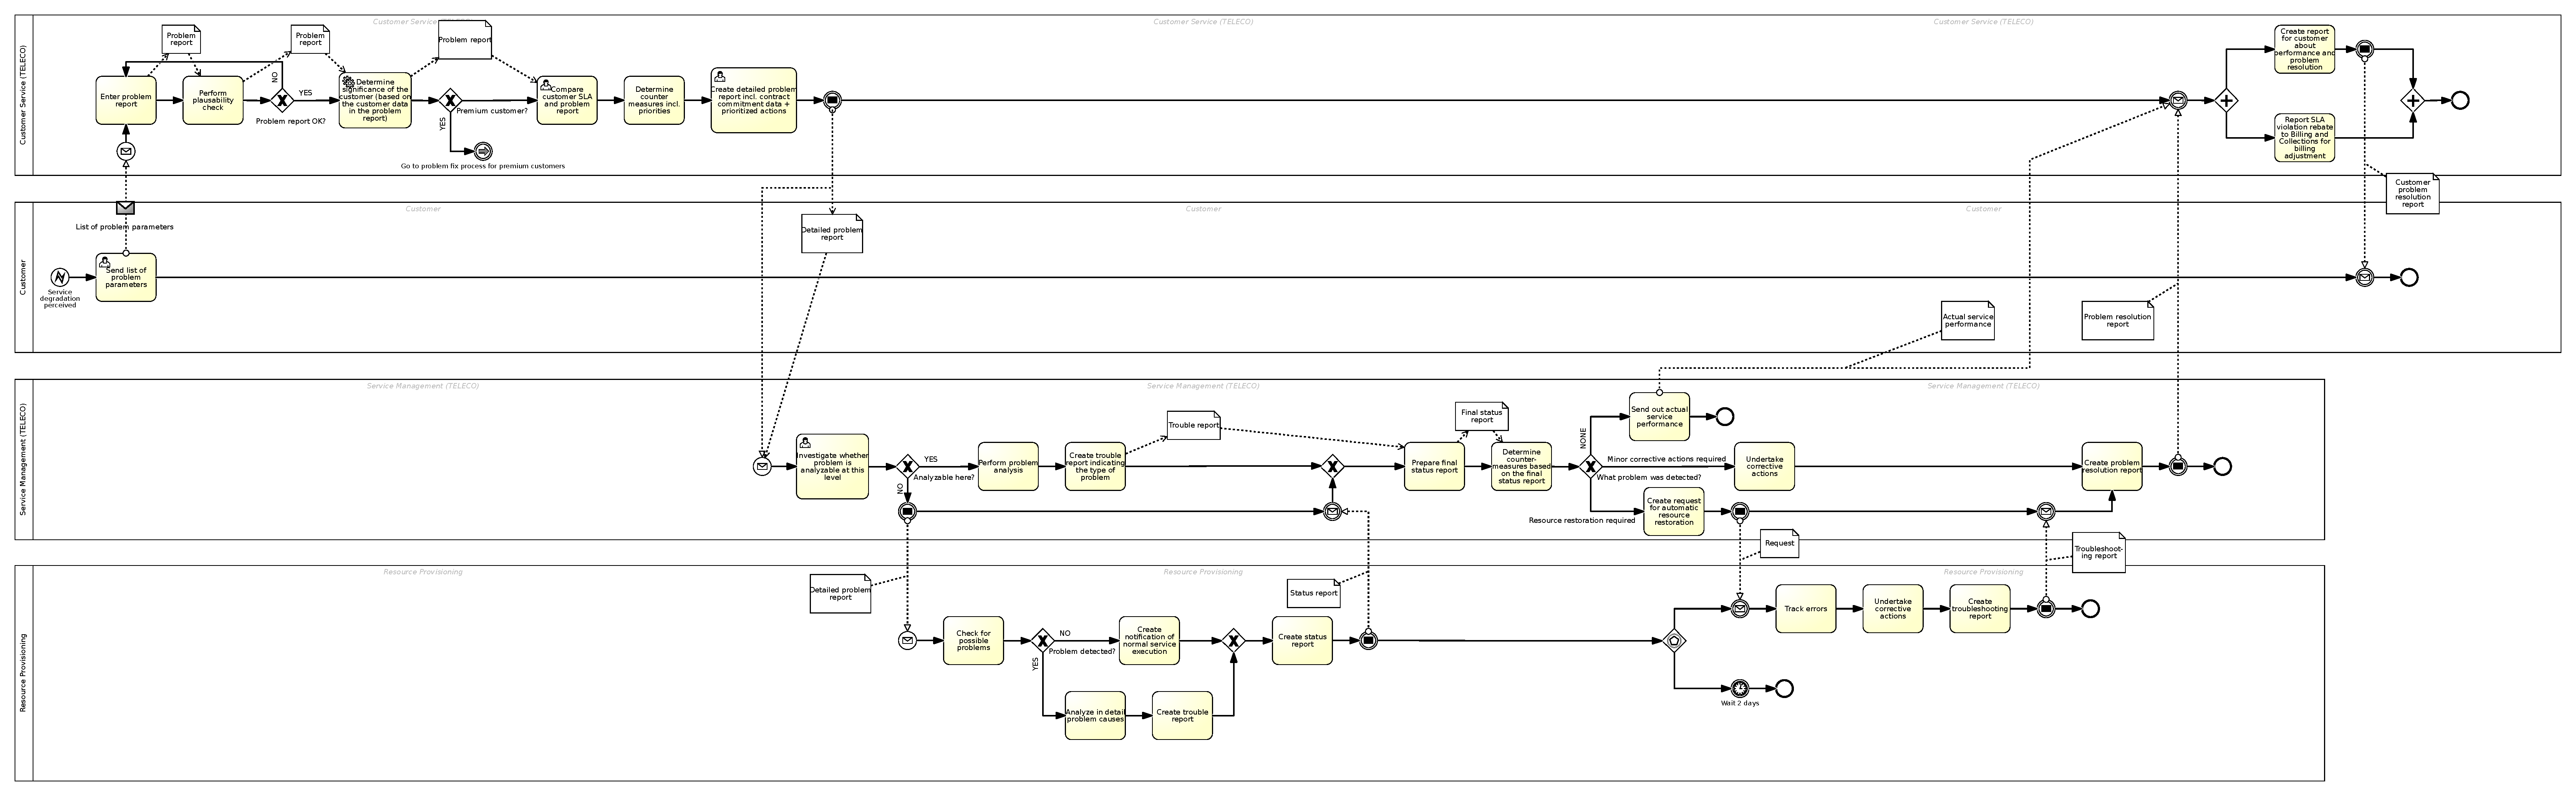
\includegraphics[width=0.95\textheight, angle=90]{./bpmn/model5.pdf}
	\caption{Hand-made BPMN diagram for process model 5}
	\label{bpmn:model5}
\end{figure}

\section{Model 6}
\begin{tcolorbox}[
	breakable,
	arc=0mm,
	left=1pt,
	right = 1pt,
	boxrule=0mm,
	colback = {white},
	]
	\texttt{\input{./models/model6.txt}}
\end{tcolorbox}
\captionof{textdesc}{Text description for model 6}
\label{txt:model6}
\newpage

{\scriptsize
	\begin{longtable}{|p{0.03 \hsize}|p{0.25 \hsize}|p{0.15 \hsize}|p{0.2 \hsize}|p{0.1 \hsize}|p{0.1 \hsize}|}
		\hline
		Order & Activity & Condition & Who & Subprocess & Terminated.
		\\\hline\hline
		\csvreader[late after line=\\\hline]
		{./results/model6_intermediate_model.csv}
		{Order=\Order,Activity=\Activity,Condition=\Condition,Who=\Who,Subprocess=\Subprocess,Terminated=\Terminated}
		{\Order & \Activity & \Condition & \Who & \Subprocess & \Terminated}
		\caption{Spreadsheet-based description for process model 6}
		\label{csv:model6}
	\end{longtable}
}

\begin{figure}[H]
	\centering
	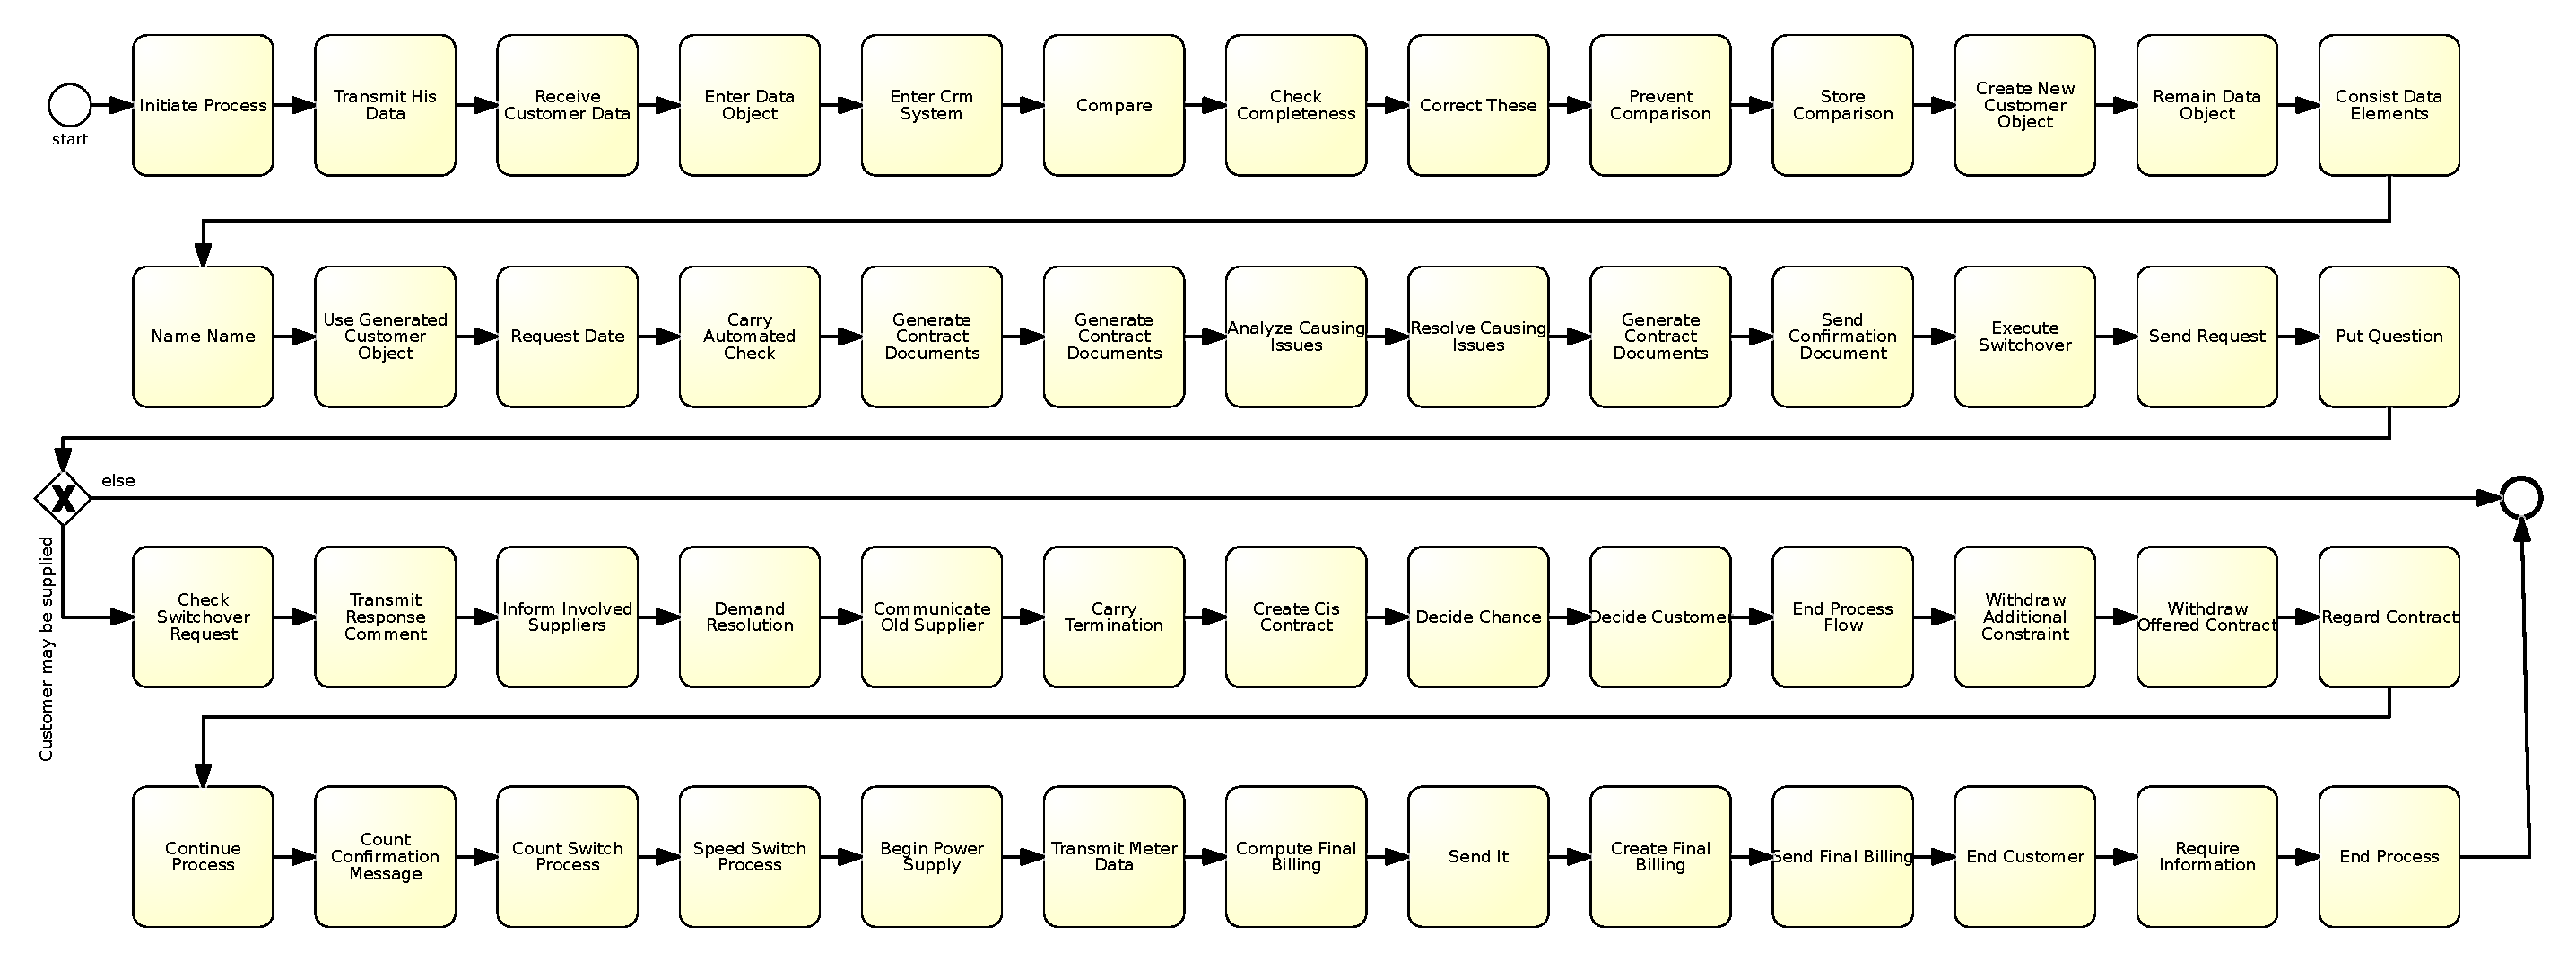
\includegraphics[width=0.95\textheight, angle=90]{./generated_bpmn/model6.pdf}
	\caption{BPMN diagram for process model 6 generated from spreadsheet-based model}
	\label{bpmn:generated_model6}
\end{figure}

\begin{figure}[H]
	\centering
	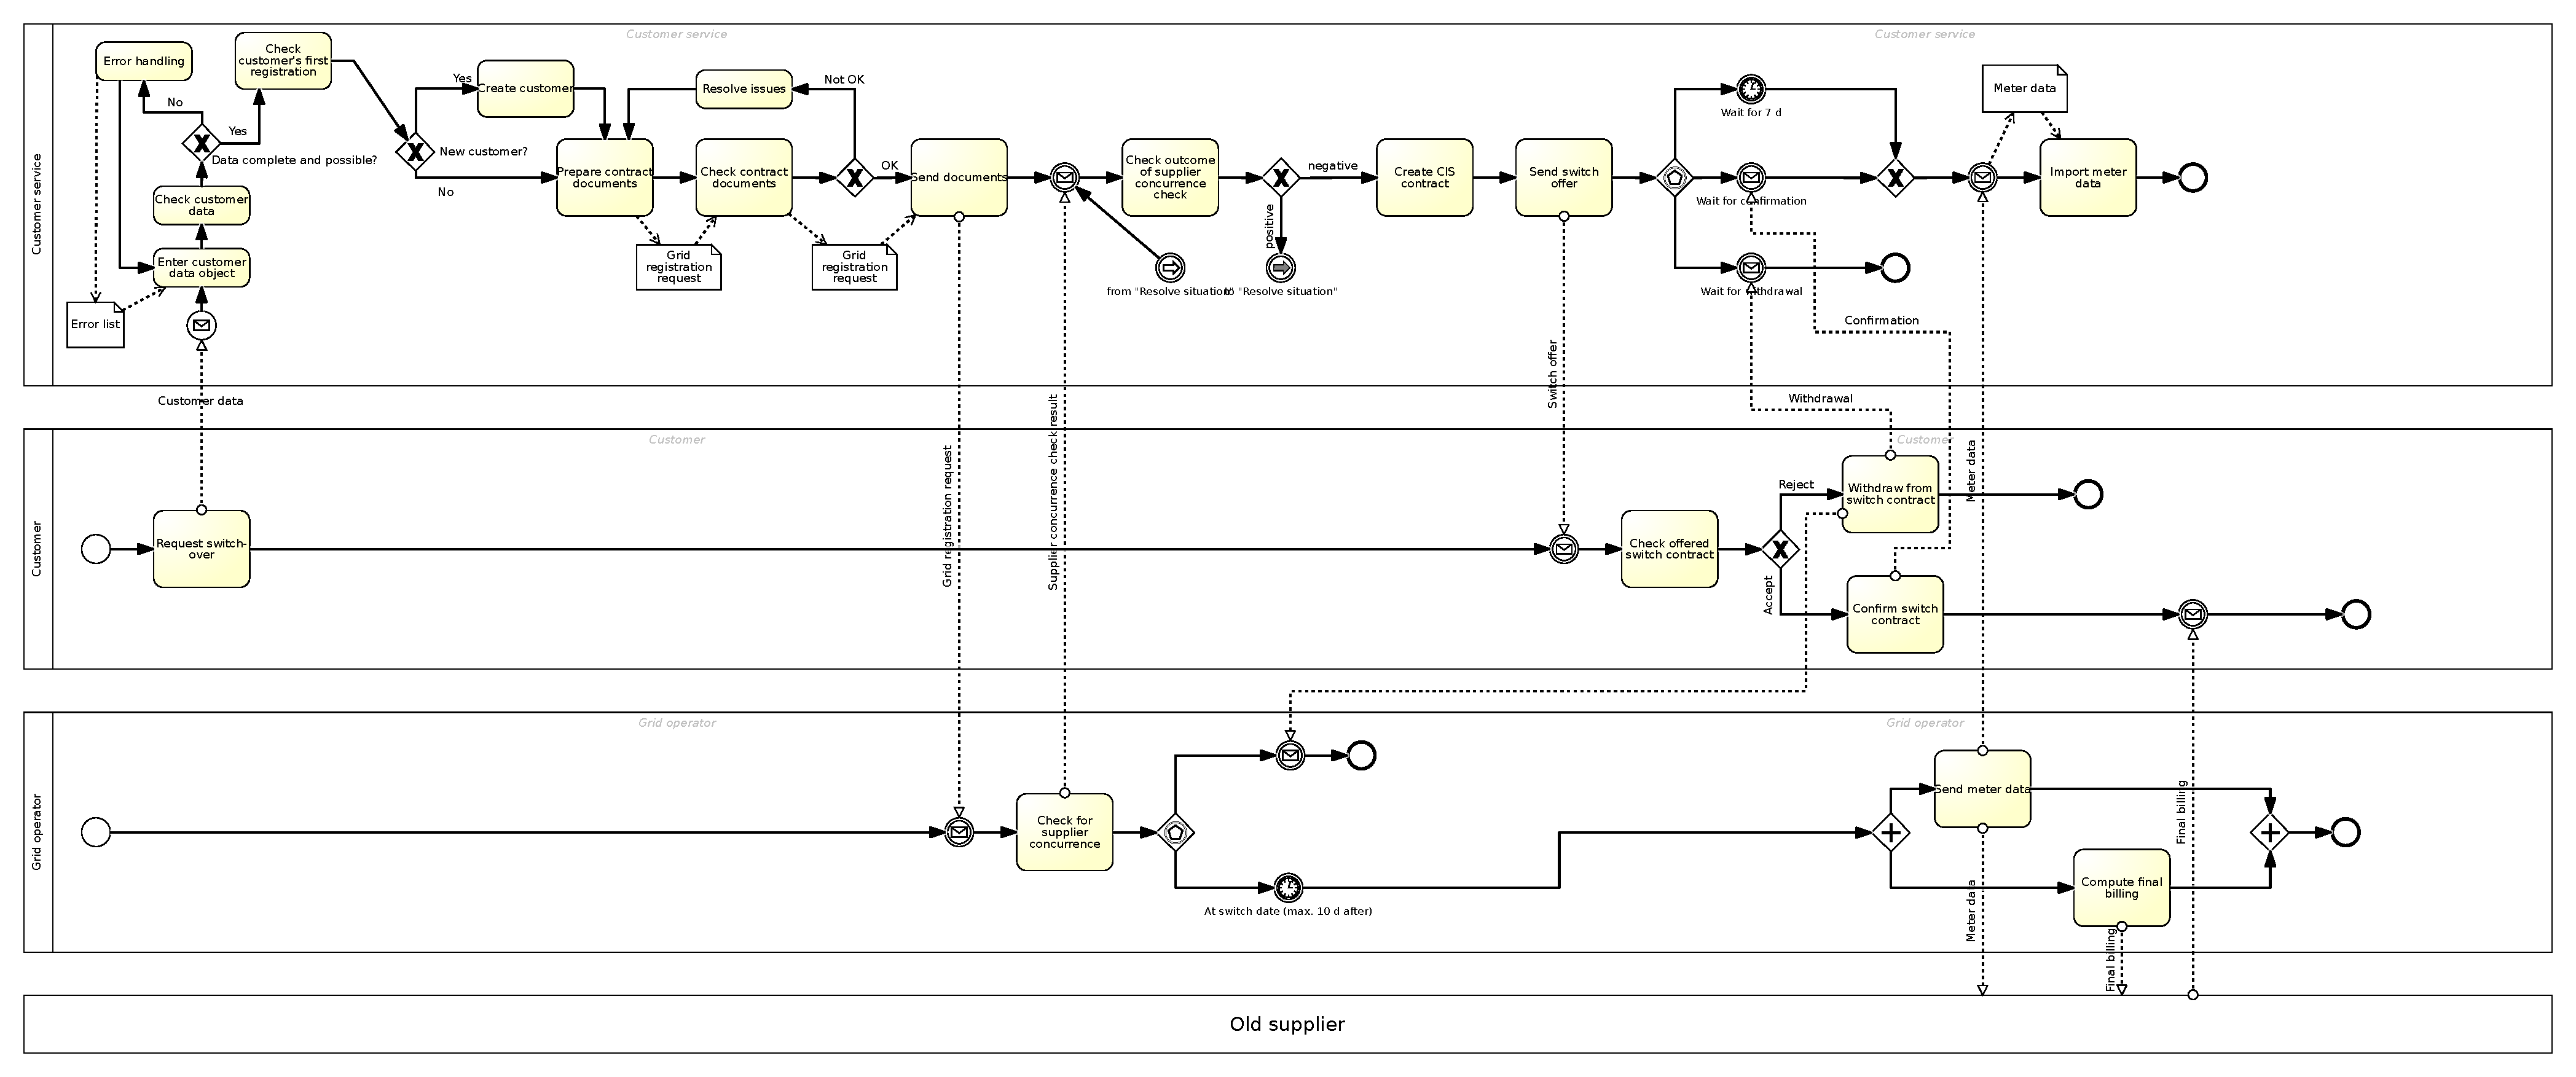
\includegraphics[width=0.95\textheight, angle=90]{./bpmn/model6.pdf}
	\caption{Hand-made BPMN diagram for process model 6}
	\label{bpmn:model6}
\end{figure}

\section{Model 7}
\begin{tcolorbox}[
	breakable,
	arc=0mm,
	left=1pt,
	right = 1pt,
	boxrule=0mm,
	colback = {white},
	]
	\texttt{\input{./models/model7.txt}}
\end{tcolorbox}
\captionof{textdesc}{Text description for model 7}
\label{txt:model7}

{\scriptsize
	\begin{longtable}{|p{0.03 \hsize}|p{0.25 \hsize}|p{0.15 \hsize}|p{0.2 \hsize}|p{0.1 \hsize}|p{0.1 \hsize}|}
		\hline
		Order & Activity & Condition & Who & Subprocess & Terminated.
		\\\hline\hline
		\csvreader[late after line=\\\hline]
		{./results/model7_intermediate_model.csv}
		{Order=\Order,Activity=\Activity,Condition=\Condition,Who=\Who,Subprocess=\Subprocess,Terminated=\Terminated}
		{\Order & \Activity & \Condition & \Who & \Subprocess & \Terminated}
		\caption{Spreadsheet-based description for process model 7}
		\label{csv:model7}
	\end{longtable}
}

\begin{figure}[H]
	\centering
	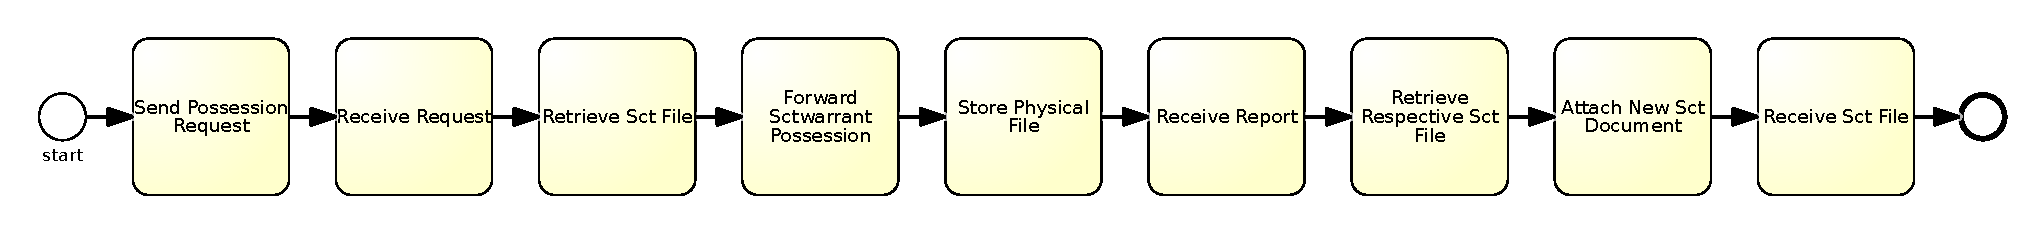
\includegraphics[width=\hsize]{./generated_bpmn/model7.pdf}
	\caption{BPMN diagram for process model 7 generated from spreadsheet-based model}
	\label{bpmn:generated_model7}
\end{figure}

\begin{figure}[H]
	\centering
	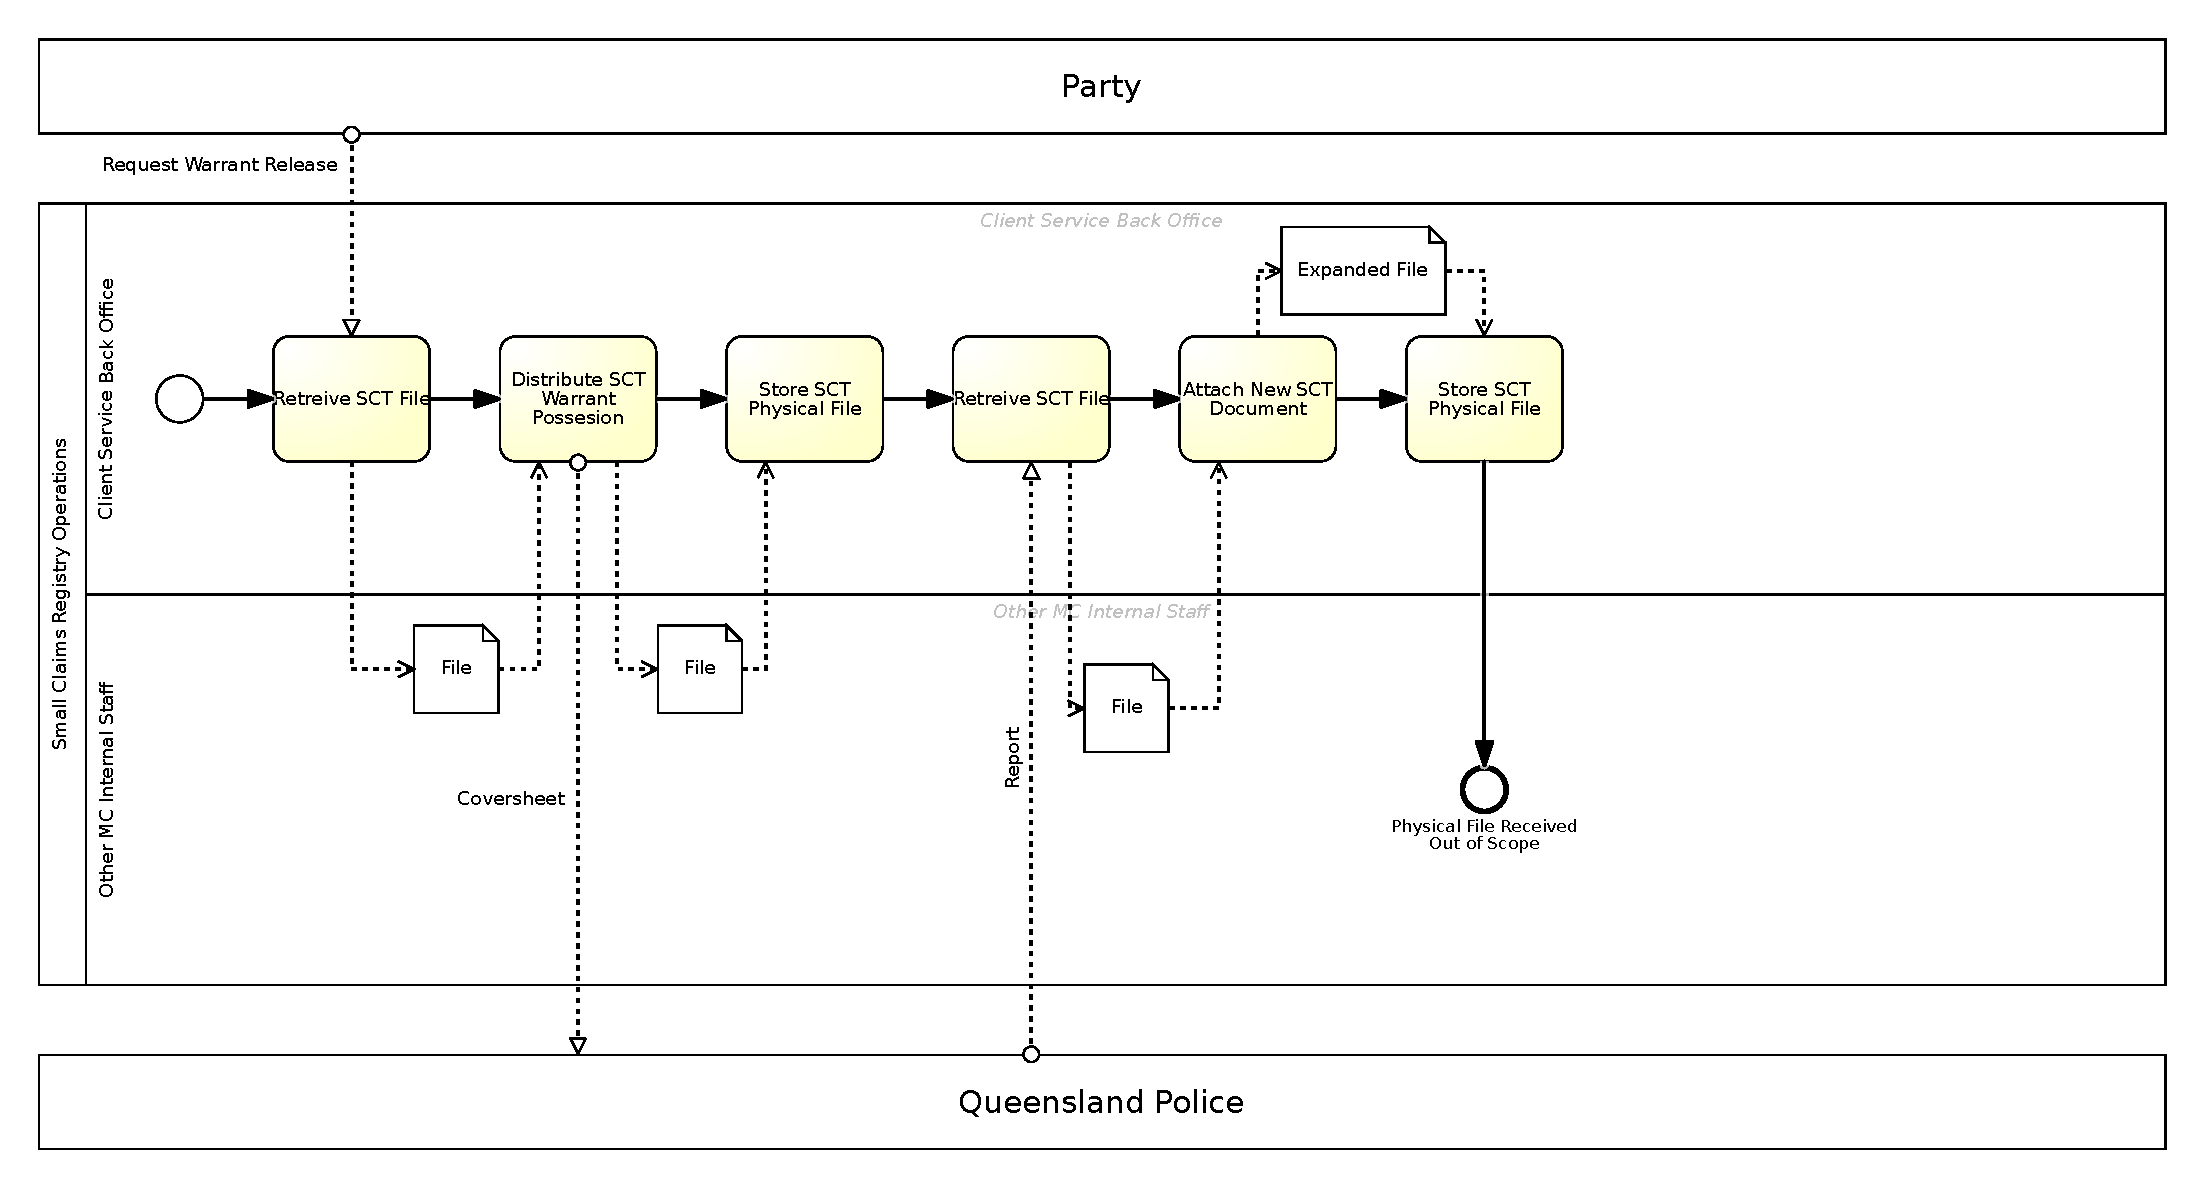
\includegraphics[width=\hsize]{./bpmn/model7.pdf}
	\caption{Hand-made BPMN diagram for process model 7}
	\label{bpmn:model7}
\end{figure}

\section{Model 8}
\begin{tcolorbox}[
	breakable,
	arc=0mm,
	left=1pt,
	right = 1pt,
	boxrule=0mm,
	colback = {white},
	]
	\texttt{\input{./models/model8.txt}}
\end{tcolorbox}
\captionof{textdesc}{Text description for model 8}
\label{txt:model8}
\newpage
{\scriptsize
	\begin{longtable}{|p{0.03 \hsize}|p{0.25 \hsize}|p{0.15 \hsize}|p{0.2 \hsize}|p{0.1 \hsize}|p{0.1 \hsize}|}
		\hline
		Order & Activity & Condition & Who & Subprocess & Terminated.
		\\\hline\hline
		\csvreader[late after line=\\\hline]
		{./results/model8_intermediate_model.csv}
		{Order=\Order,Activity=\Activity,Condition=\Condition,Who=\Who,Subprocess=\Subprocess,Terminated=\Terminated}
		{\Order & \Activity & \Condition & \Who & \Subprocess & \Terminated}
		\caption{Spreadsheet-based description for process model 8}
		\label{csv:model8}
	\end{longtable}
}

\begin{figure}[H]
	\centering
	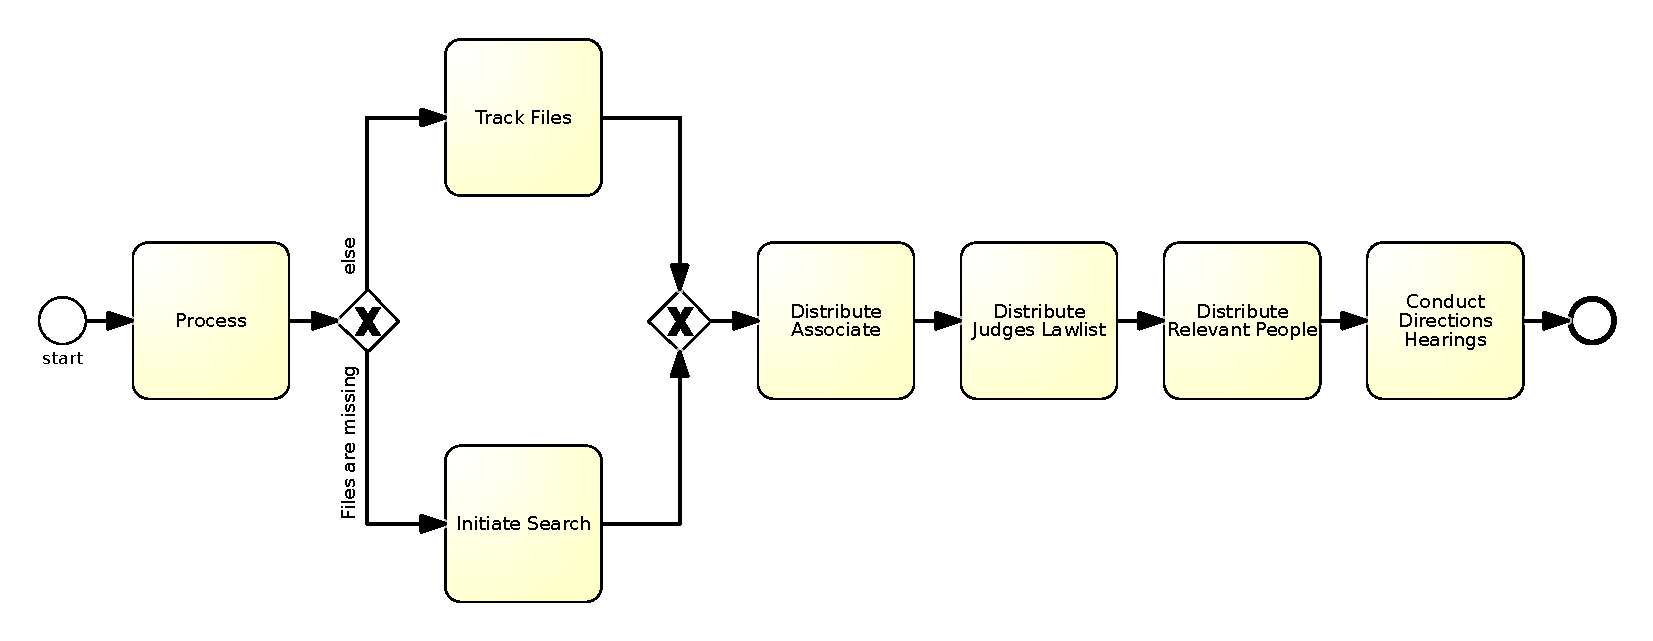
\includegraphics[width=\hsize]{./generated_bpmn/model8.pdf}
	\caption{BPMN diagram for process model 8 generated from spreadsheet-based model}
	\label{bpmn:generated_model8}
\end{figure}

\begin{figure}[H]
	\centering
	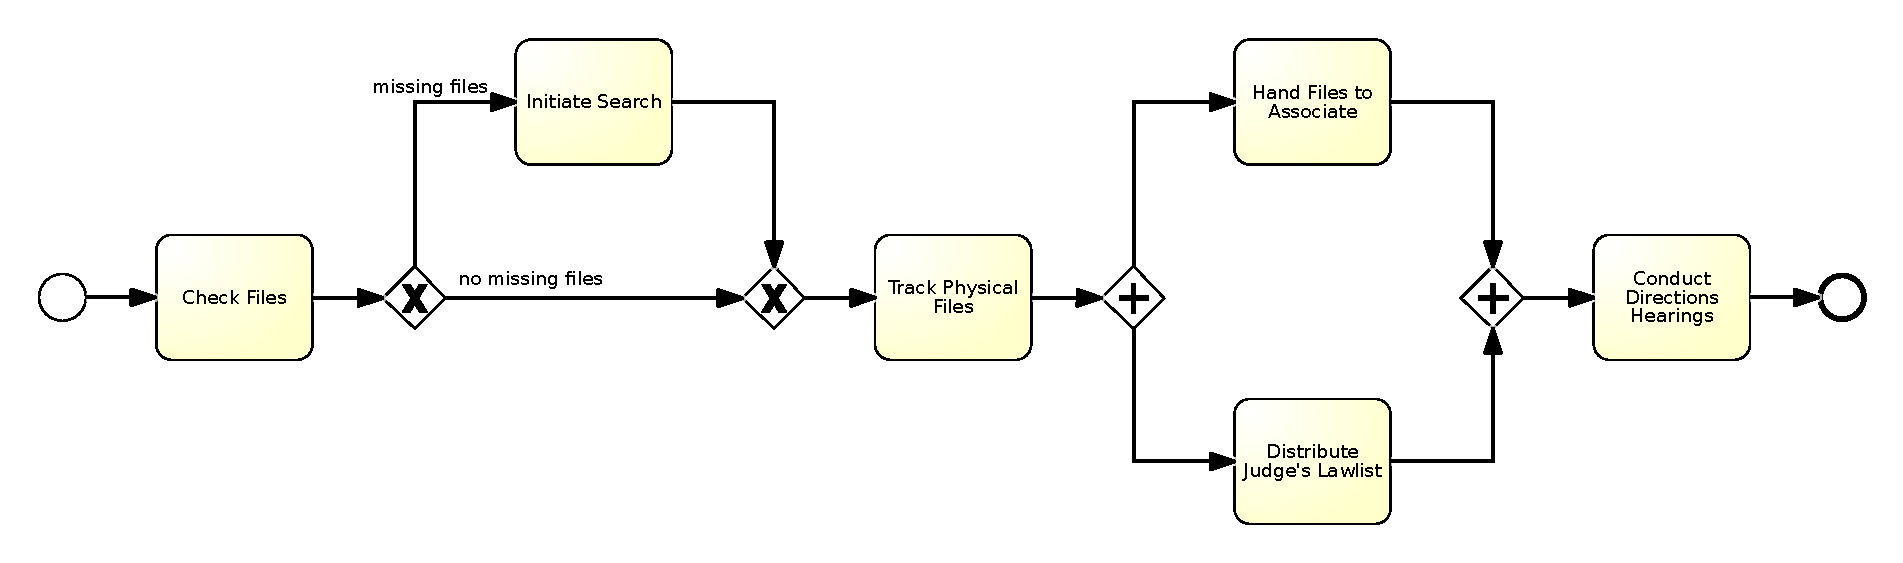
\includegraphics[width=\hsize]{./bpmn/model8.pdf}
	\caption{Hand-made BPMN diagram for process model 8}
	\label{bpmn:model8}
\end{figure}

\section{Model 9}
\begin{tcolorbox}[
	breakable,
	arc=0mm,
	left=1pt,
	right = 1pt,
	boxrule=0mm,
	colback = {white},
	]
	\texttt{\input{./models/model9.txt}}
\end{tcolorbox}
\captionof{textdesc}{Text description for model 9}
\label{txt:model9}

{\scriptsize
	\begin{longtable}{|p{0.03 \hsize}|p{0.25 \hsize}|p{0.15 \hsize}|p{0.2 \hsize}|p{0.1 \hsize}|p{0.1 \hsize}|}
		\hline
		Order & Activity & Condition & Who & Subprocess & Terminated.
		\\\hline\hline
		\csvreader[late after line=\\\hline]
		{./results/model9_intermediate_model.csv}
		{Order=\Order,Activity=\Activity,Condition=\Condition,Who=\Who,Subprocess=\Subprocess,Terminated=\Terminated}
		{\Order & \Activity & \Condition & \Who & \Subprocess & \Terminated}
		\caption{Spreadsheet-based description for process model 9}
		\label{csv:model9}
	\end{longtable}
}

\begin{figure}[H]
	\centering
	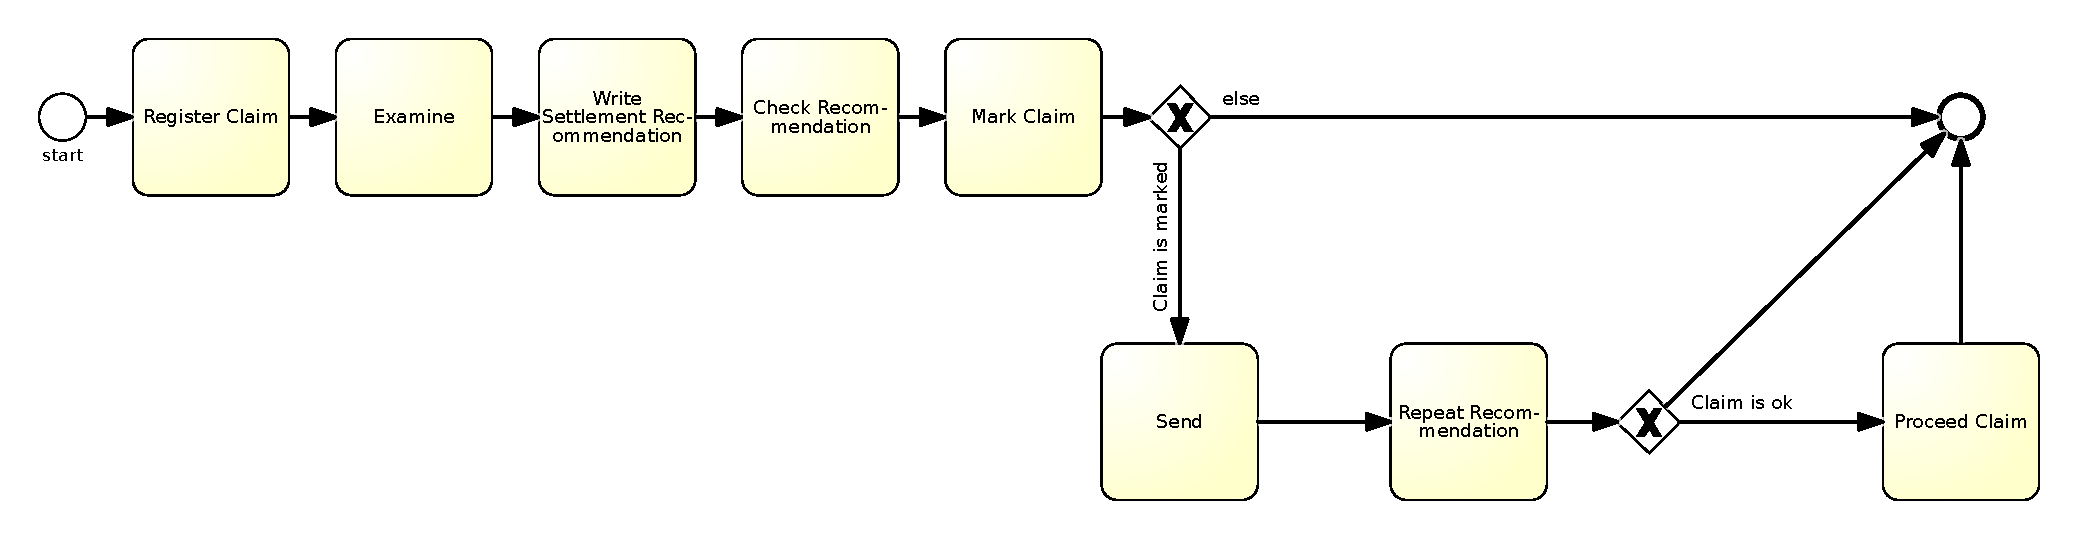
\includegraphics[width=\hsize]{./generated_bpmn/model9.pdf}
	\caption{BPMN diagram for process model 9 generated from spreadsheet-based model}
	\label{bpmn:generated_model9}
\end{figure}

\begin{figure}[H]
	\centering
	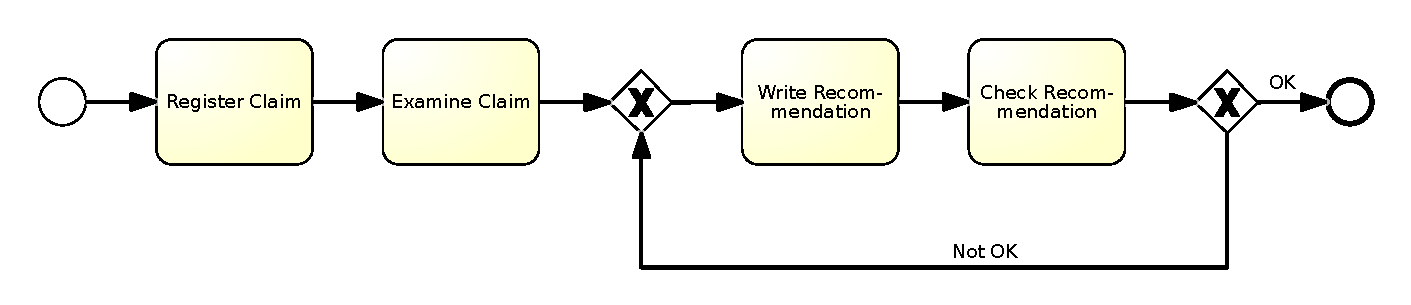
\includegraphics[width=\hsize]{./bpmn/model9.pdf}
	\caption{Hand-made BPMN diagram for process model 9}
	\label{bpmn:model9}
\end{figure}

\section{Model 10}
\begin{tcolorbox}[
	breakable,
	arc=0mm,
	left=1pt,
	right = 1pt,
	boxrule=0mm,
	colback = {white},
	]
	\texttt{\input{./models/model10.txt}}
\end{tcolorbox}
\captionof{textdesc}{Text description for model 10}
\label{txt:model10}

{\scriptsize
	\begin{longtable}{|p{0.03 \hsize}|p{0.25 \hsize}|p{0.15 \hsize}|p{0.2 \hsize}|p{0.1 \hsize}|p{0.1 \hsize}|}
		\hline
		Order & Activity & Condition & Who & Subprocess & Terminated.
		\\\hline\hline
		\csvreader[late after line=\\\hline]
		{./results/model10_intermediate_model.csv}
		{Order=\Order,Activity=\Activity,Condition=\Condition,Who=\Who,Subprocess=\Subprocess,Terminated=\Terminated}
		{\Order & \Activity & \Condition & \Who & \Subprocess & \Terminated}
		\caption{Spreadsheet-based description for process model 10}
		\label{csv:model10}
	\end{longtable}
}

\begin{figure}[H]
	\centering
	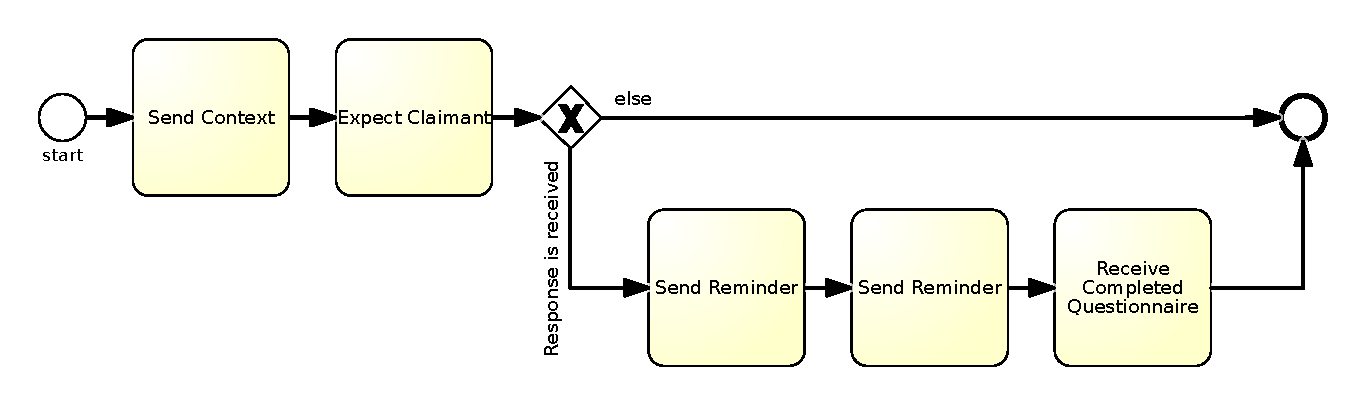
\includegraphics[width=\hsize]{./generated_bpmn/model10.pdf}
	\caption{BPMN diagram for process model 10 generated from spreadsheet-based model}
	\label{bpmn:generated_model10}
\end{figure}

\begin{figure}[H]
	\centering
	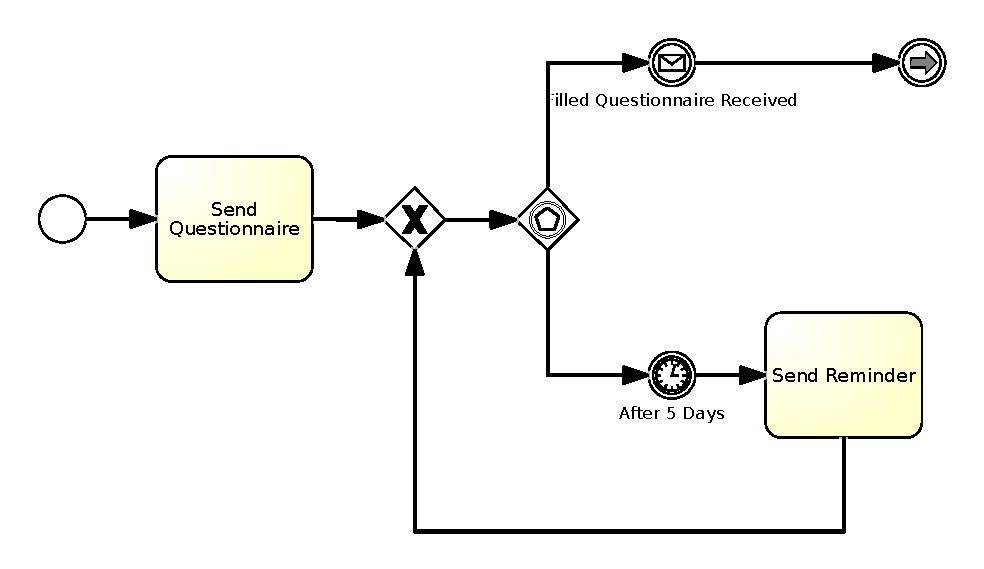
\includegraphics[width=\hsize]{./bpmn/model10.pdf}
	\caption{Hand-made BPMN diagram for process model 10}
	\label{bpmn:model10}
\end{figure}

\section{Model 11}
\begin{tcolorbox}[
	breakable,
	arc=0mm,
	left=1pt,
	right = 1pt,
	boxrule=0mm,
	colback = {white},
	]
	\texttt{\input{./models/model11.txt}}
\end{tcolorbox}
\captionof{textdesc}{Text description for model 11}
\label{txt:model11}

{\scriptsize
	\begin{longtable}{|p{0.03 \hsize}|p{0.25 \hsize}|p{0.15 \hsize}|p{0.2 \hsize}|p{0.1 \hsize}|p{0.1 \hsize}|}
		\hline
		Order & Activity & Condition & Who & Subprocess & Terminated.
		\\\hline\hline
		\csvreader[late after line=\\\hline]
		{./results/model11_intermediate_model.csv}
		{Order=\Order,Activity=\Activity,Condition=\Condition,Who=\Who,Subprocess=\Subprocess,Terminated=\Terminated}
		{\Order & \Activity & \Condition & \Who & \Subprocess & \Terminated}
		\caption{Spreadsheet-based description for process model 11}
		\label{csv:model11}
	\end{longtable}
}

\begin{figure}[H]
	\centering
	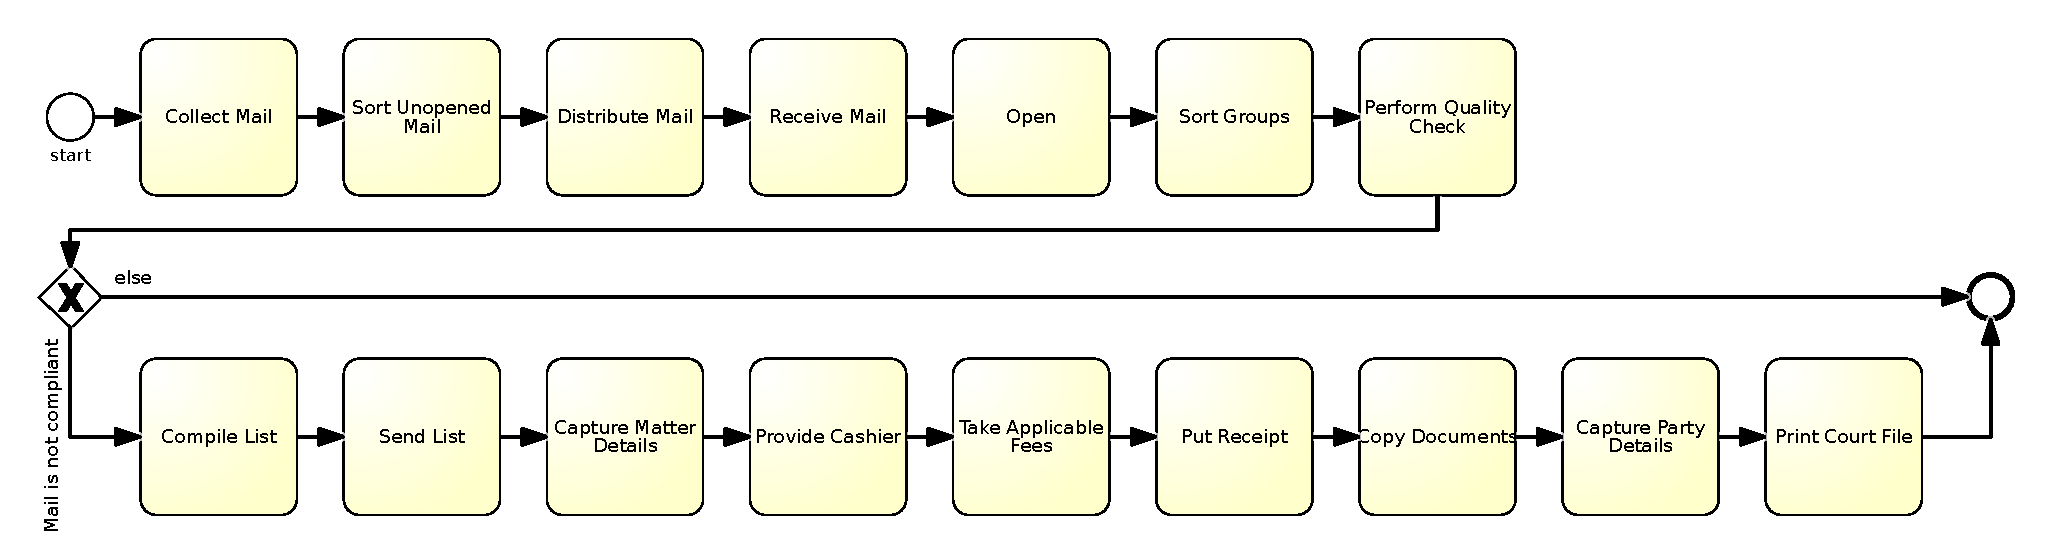
\includegraphics[width=\hsize]{./generated_bpmn/model11.pdf}
	\caption{BPMN diagram for process model 11 generated from spreadsheet-based model}
	\label{bpmn:generated_model11}
\end{figure}

\begin{figure}[H]
	\centering
	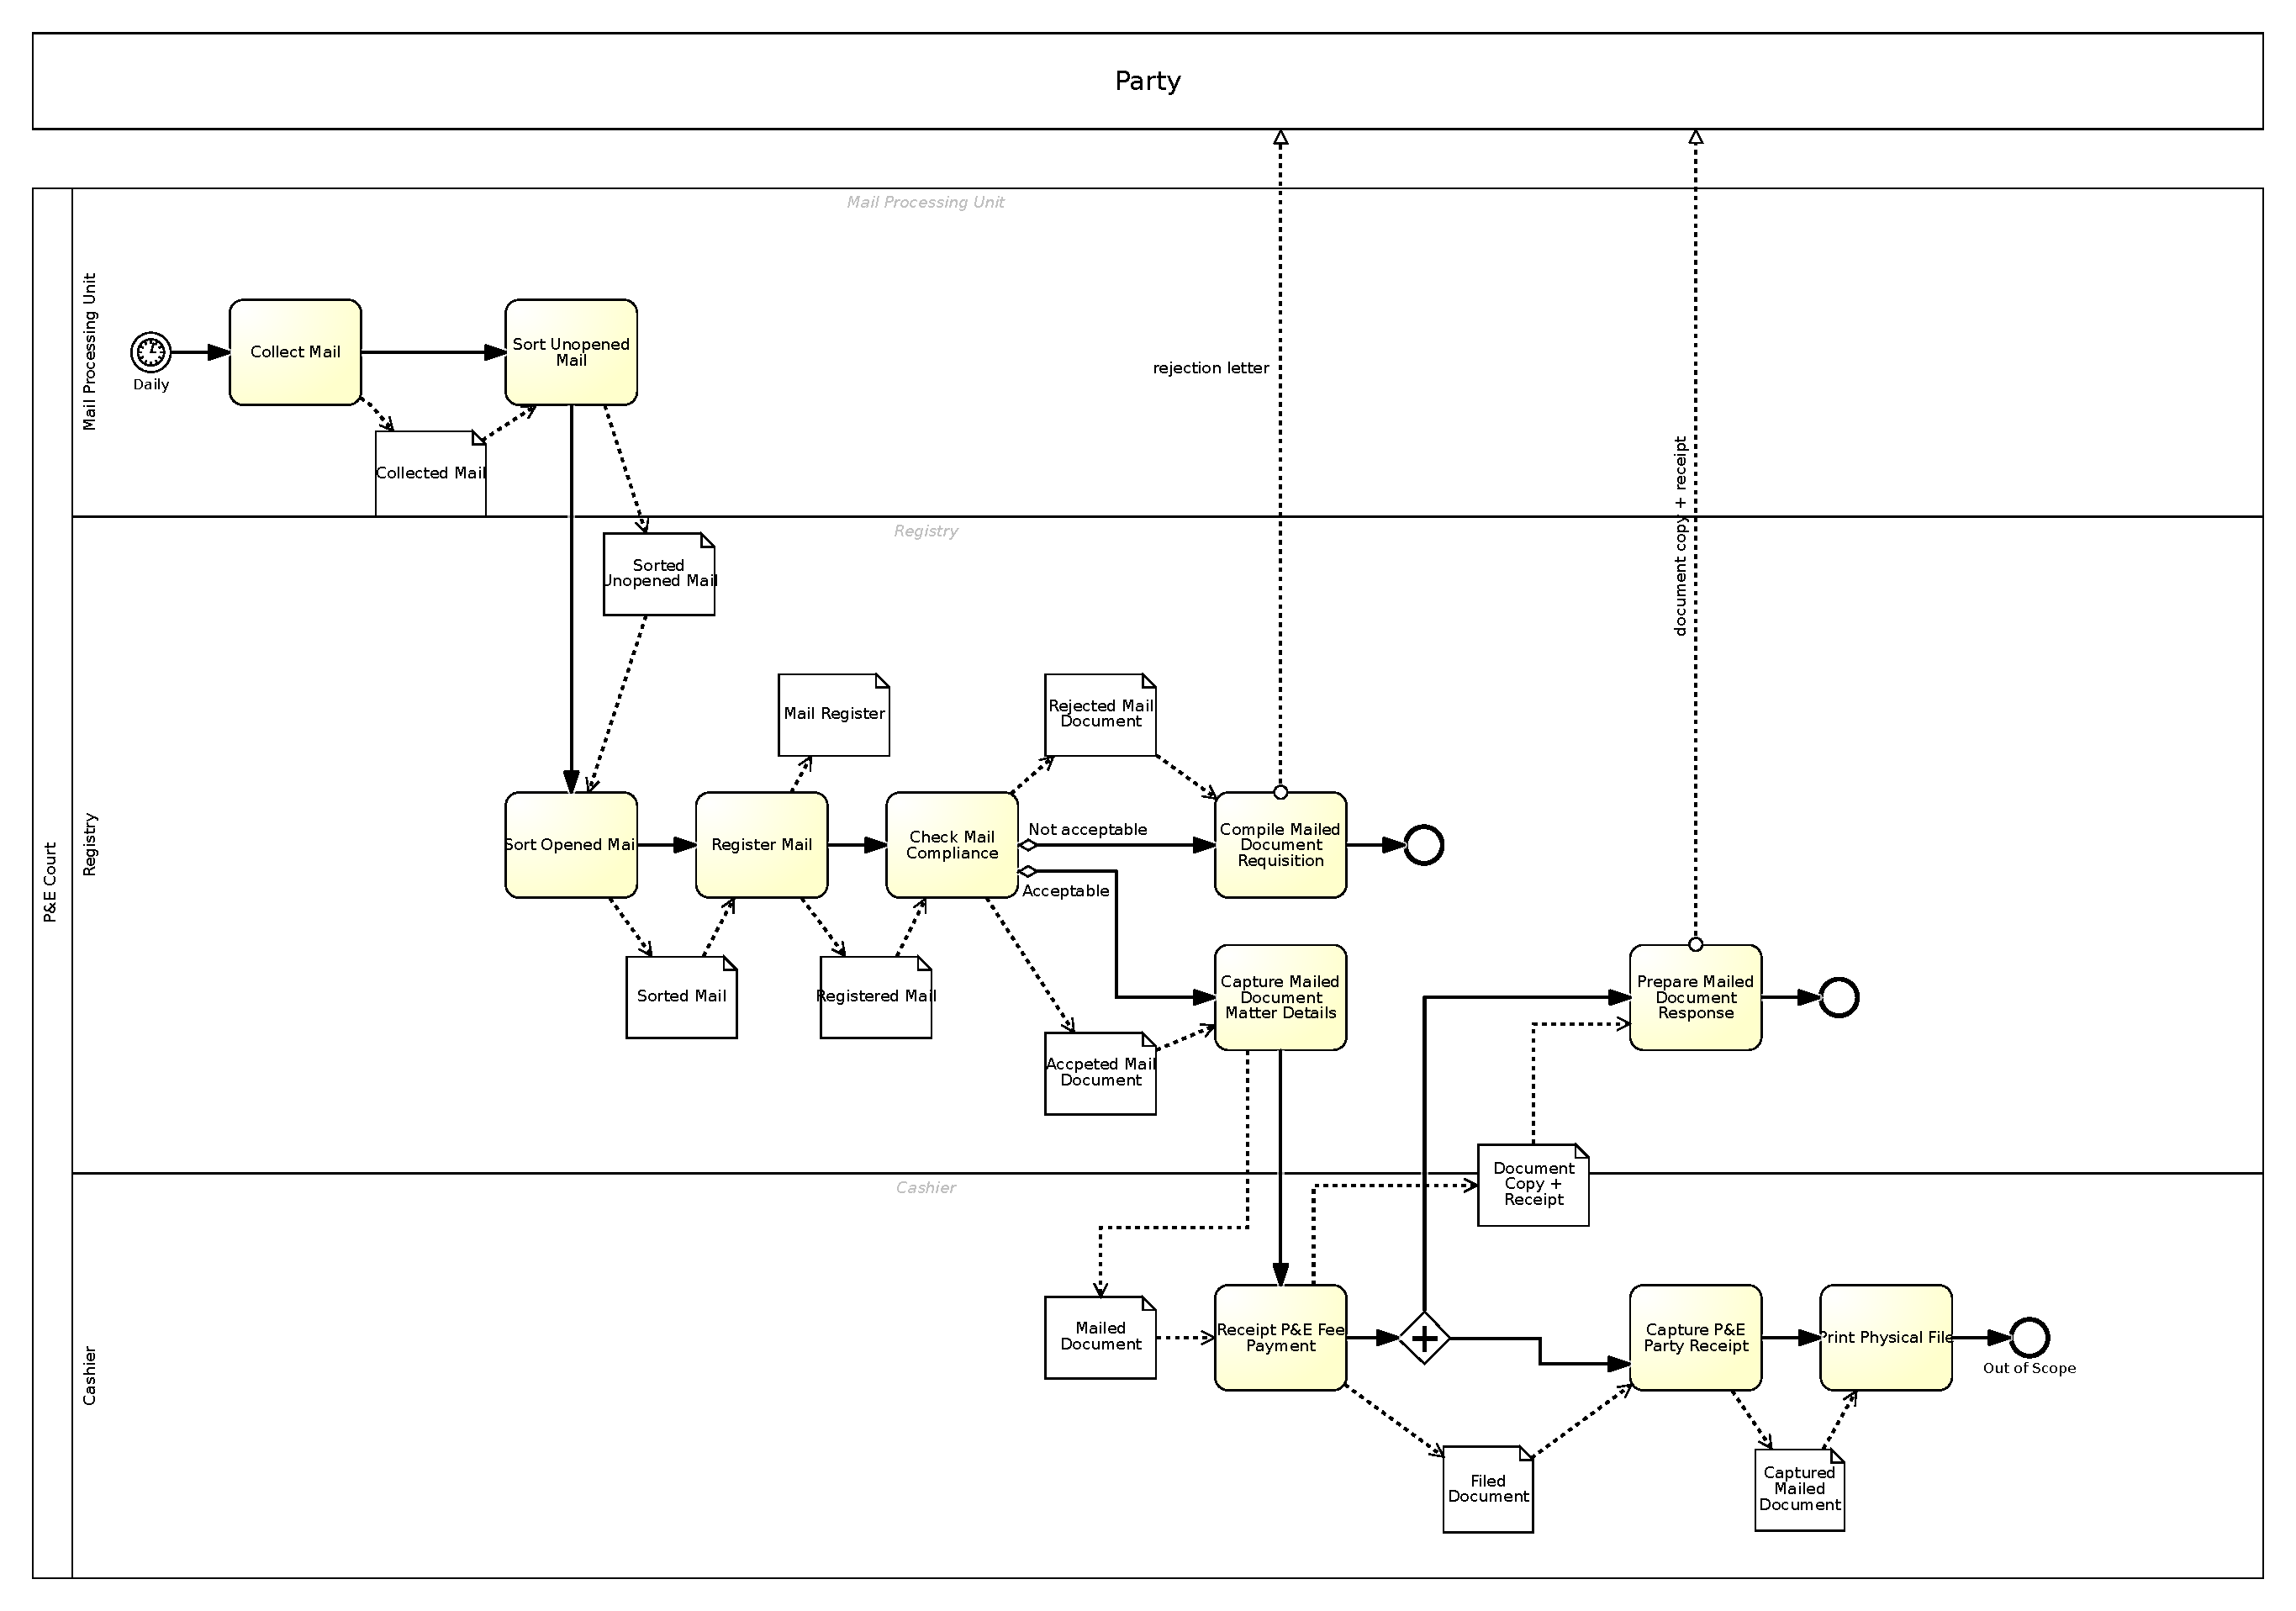
\includegraphics[width=\hsize]{./bpmn/model11.pdf}
	\caption{Hand-made BPMN diagram for process model 11}
	\label{bpmn:model11}
\end{figure}

\section{Model 12}
\begin{tcolorbox}[
	breakable,
	arc=0mm,
	left=1pt,
	right = 1pt,
	boxrule=0mm,
	colback = {white},
	]
	\texttt{\input{./models/model12.txt}}
\end{tcolorbox}
\captionof{textdesc}{Text description for model 12}
\label{txt:model12}

{\scriptsize
	\begin{longtable}{|p{0.03 \hsize}|p{0.25 \hsize}|p{0.15 \hsize}|p{0.2 \hsize}|p{0.1 \hsize}|p{0.1 \hsize}|}
		\hline
		Order & Activity & Condition & Who & Subprocess & Terminated.
		\\\hline\hline
		\csvreader[late after line=\\\hline]
		{./results/model12_intermediate_model.csv}
		{Order=\Order,Activity=\Activity,Condition=\Condition,Who=\Who,Subprocess=\Subprocess,Terminated=\Terminated}
		{\Order & \Activity & \Condition & \Who & \Subprocess & \Terminated}
		\caption{Spreadsheet-based description for process model 12}
		\label{csv:model12}
	\end{longtable}
}

\begin{figure}[H]
	\centering
	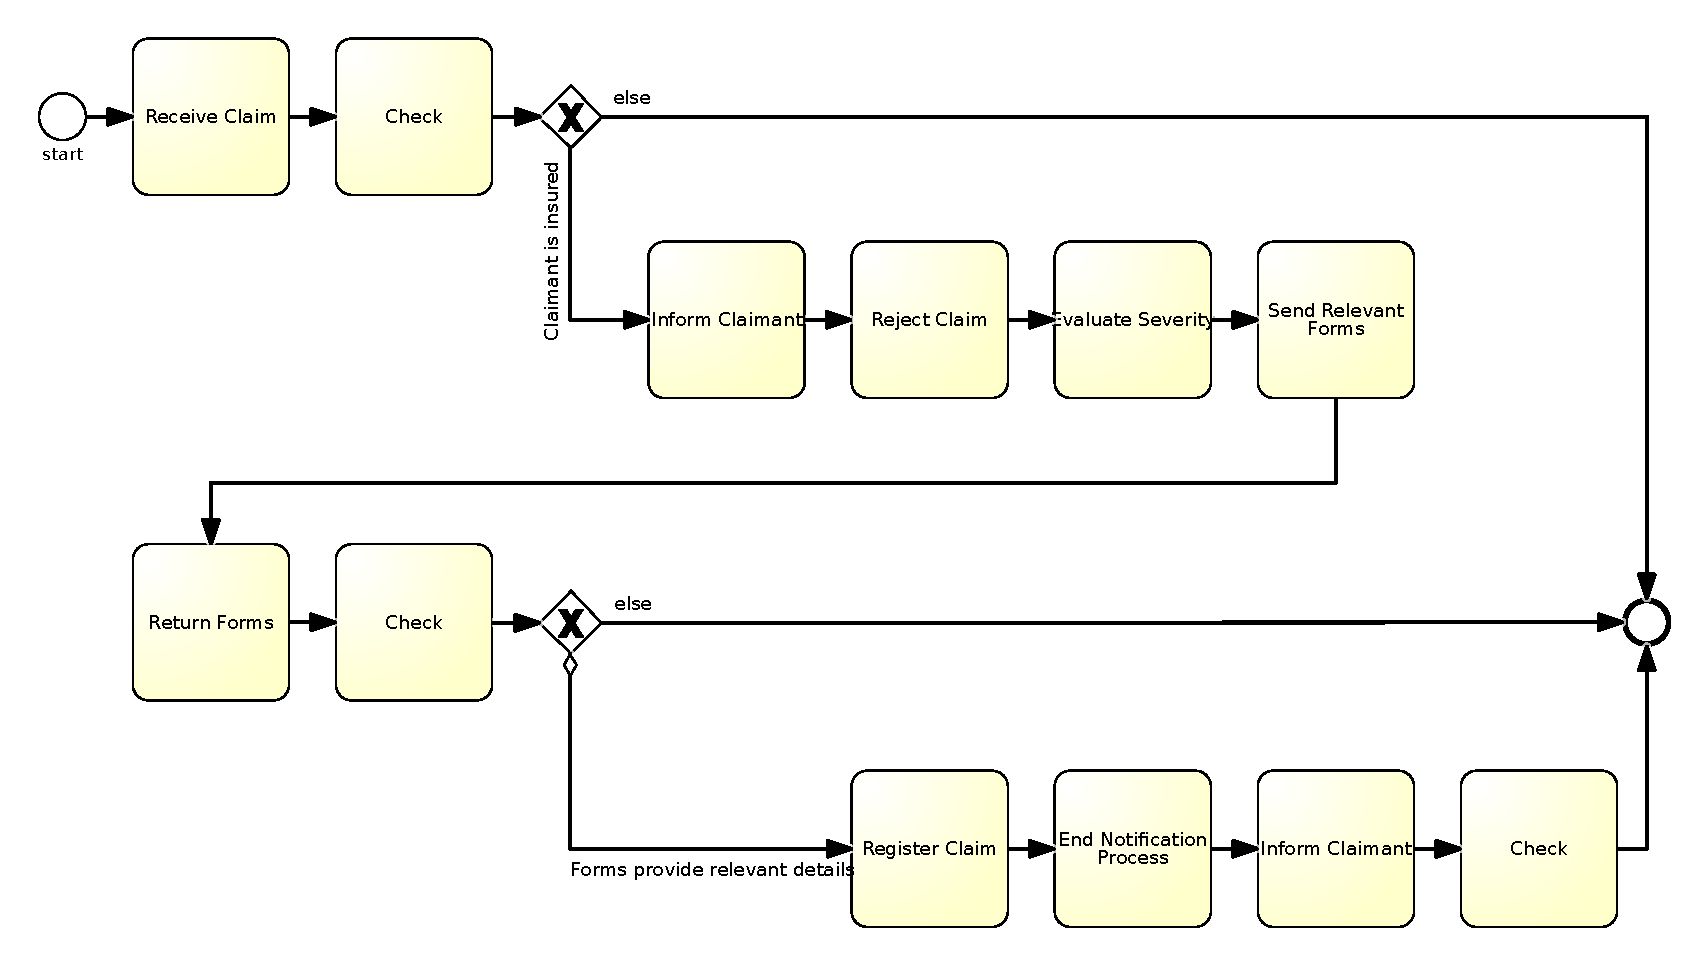
\includegraphics[width=\hsize]{./generated_bpmn/model12.pdf}
	\caption{BPMN diagram for process model 12 generated from spreadsheet-based model}
	\label{bpmn:generated_model12}
\end{figure}

\begin{figure}[H]
	\centering
	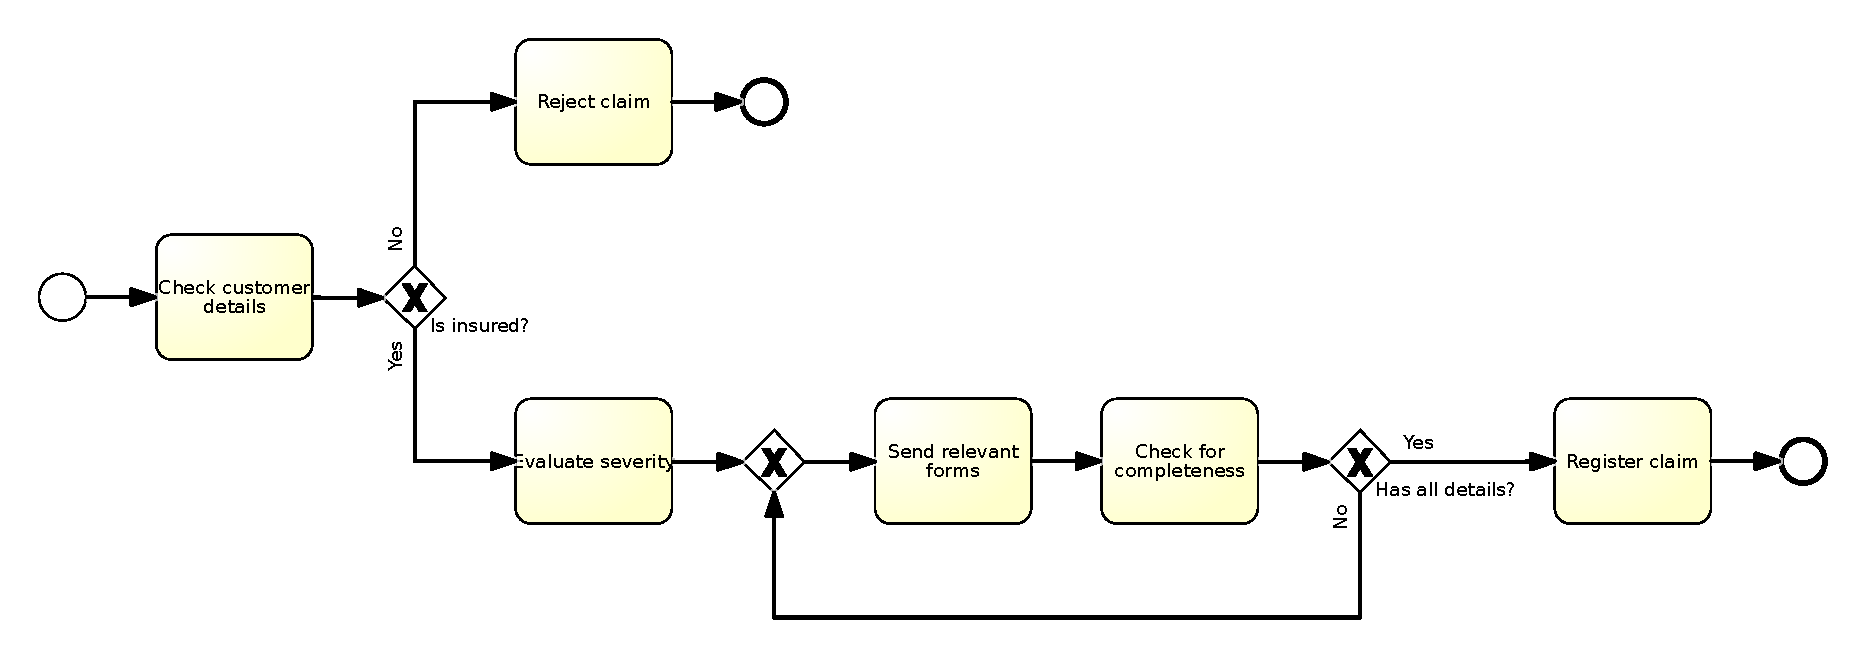
\includegraphics[width=\hsize]{./bpmn/model12.pdf}
	\caption{Hand-made BPMN diagram for process model 12}
	\label{bpmn:model12}
\end{figure}

\section{Model 13}
\begin{tcolorbox}[
	breakable,
	arc=0mm,
	left=1pt,
	right = 1pt,
	boxrule=0mm,
	colback = {white},
	]
	\texttt{\input{./models/model13.txt}}
\end{tcolorbox}
\captionof{textdesc}{Text description for model 13}
\label{txt:model13}

{\scriptsize
	\begin{longtable}{|p{0.03 \hsize}|p{0.25 \hsize}|p{0.15 \hsize}|p{0.2 \hsize}|p{0.1 \hsize}|p{0.1 \hsize}|}
		\hline
		Order & Activity & Condition & Who & Subprocess & Terminated.
		\\\hline\hline
		\csvreader[late after line=\\\hline]
		{./results/model13_intermediate_model.csv}
		{Order=\Order,Activity=\Activity,Condition=\Condition,Who=\Who,Subprocess=\Subprocess,Terminated=\Terminated}
		{\Order & \Activity & \Condition & \Who & \Subprocess & \Terminated}
		\caption{Spreadsheet-based description for process model 13}
		\label{csv:model13}
	\end{longtable}
}

\begin{figure}[H]
	\centering
	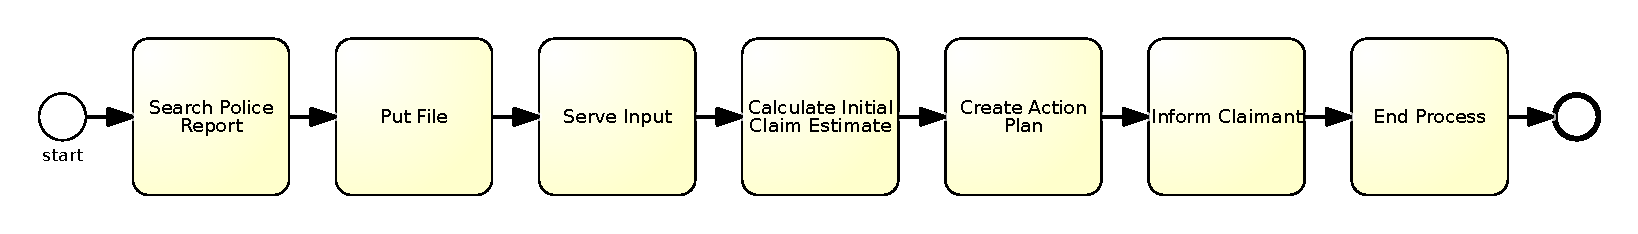
\includegraphics[width=\hsize]{./generated_bpmn/model13.pdf}
	\caption{BPMN diagram for process model 13 generated from spreadsheet-based model}
	\label{bpmn:generated_model13}
\end{figure}

\begin{figure}[H]
	\centering
	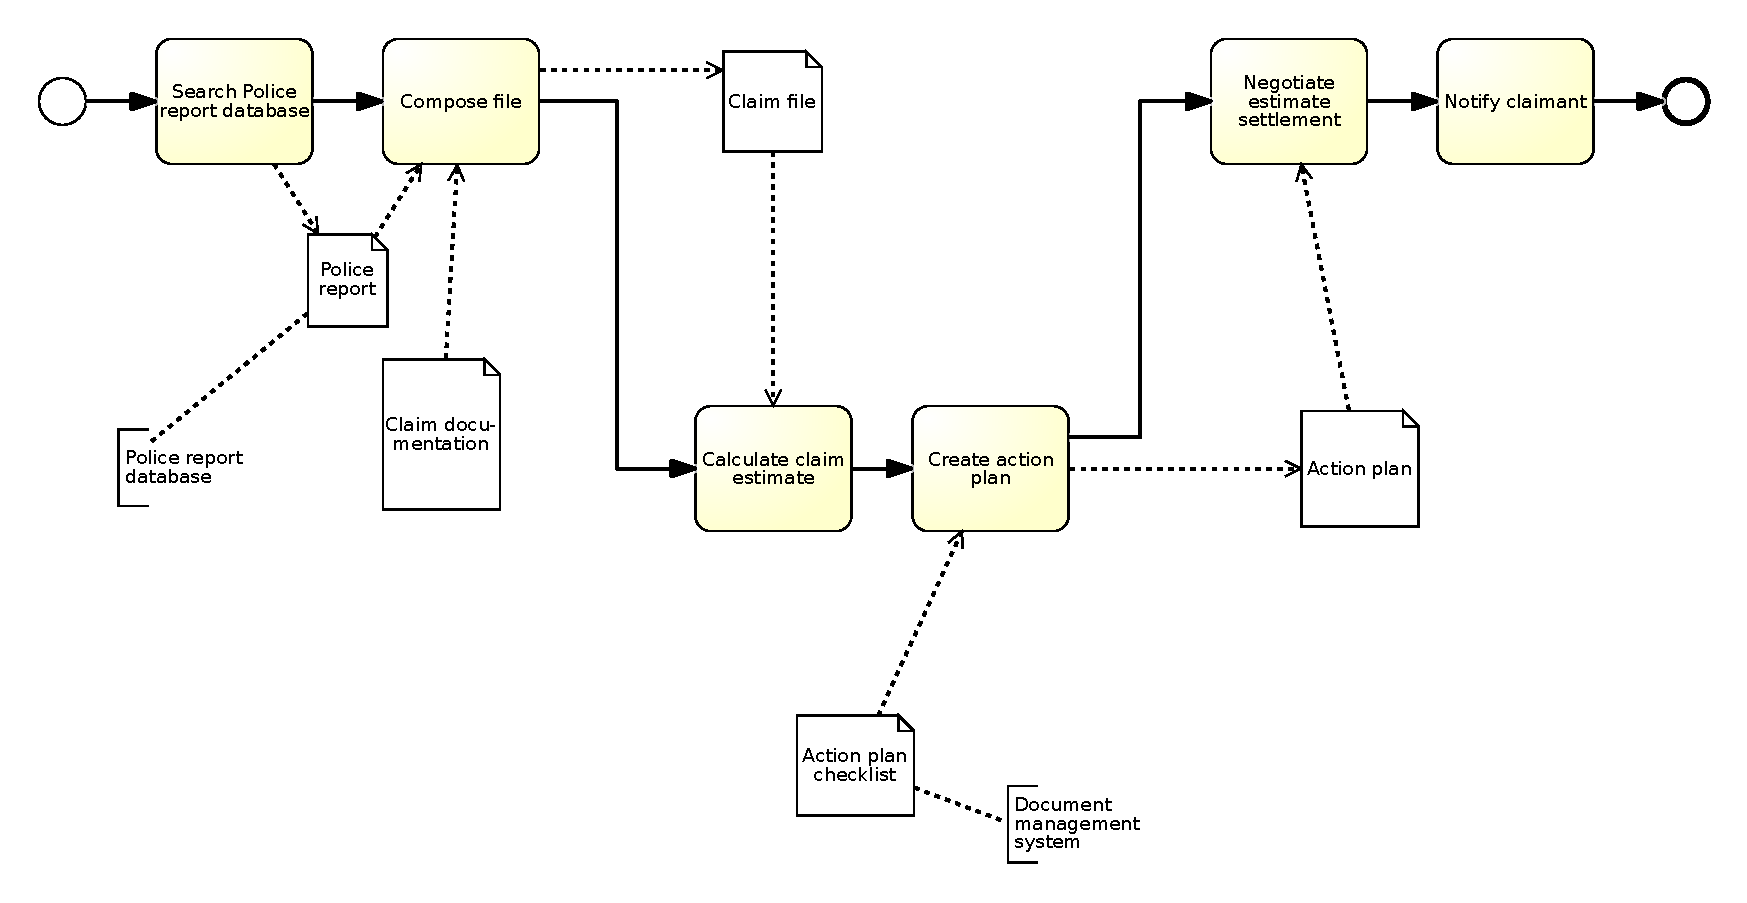
\includegraphics[width=\hsize]{./bpmn/model13.pdf}
	\caption{Hand-made BPMN diagram for process model 13}
	\label{bpmn:model13}
\end{figure}

\section{Model 14}
\begin{tcolorbox}[
	breakable,
	arc=0mm,
	left=1pt,
	right = 1pt,
	boxrule=0mm,
	colback = {white},
	]
	\texttt{\input{./models/model14.txt}}
\end{tcolorbox}
\captionof{textdesc}{Text description for model 14}
\label{txt:model14}

{\scriptsize
	\begin{longtable}{|p{0.03 \hsize}|p{0.25 \hsize}|p{0.15 \hsize}|p{0.2 \hsize}|p{0.1 \hsize}|p{0.1 \hsize}|}
		\hline
		Order & Activity & Condition & Who & Subprocess & Terminated.
		\\\hline\hline
		\csvreader[late after line=\\\hline]
		{./results/model14_intermediate_model.csv}
		{Order=\Order,Activity=\Activity,Condition=\Condition,Who=\Who,Subprocess=\Subprocess,Terminated=\Terminated}
		{\Order & \Activity & \Condition & \Who & \Subprocess & \Terminated}
		\caption{Spreadsheet-based description for process model 14}
		\label{csv:model14}
	\end{longtable}
}

\begin{figure}[H]
	\centering
	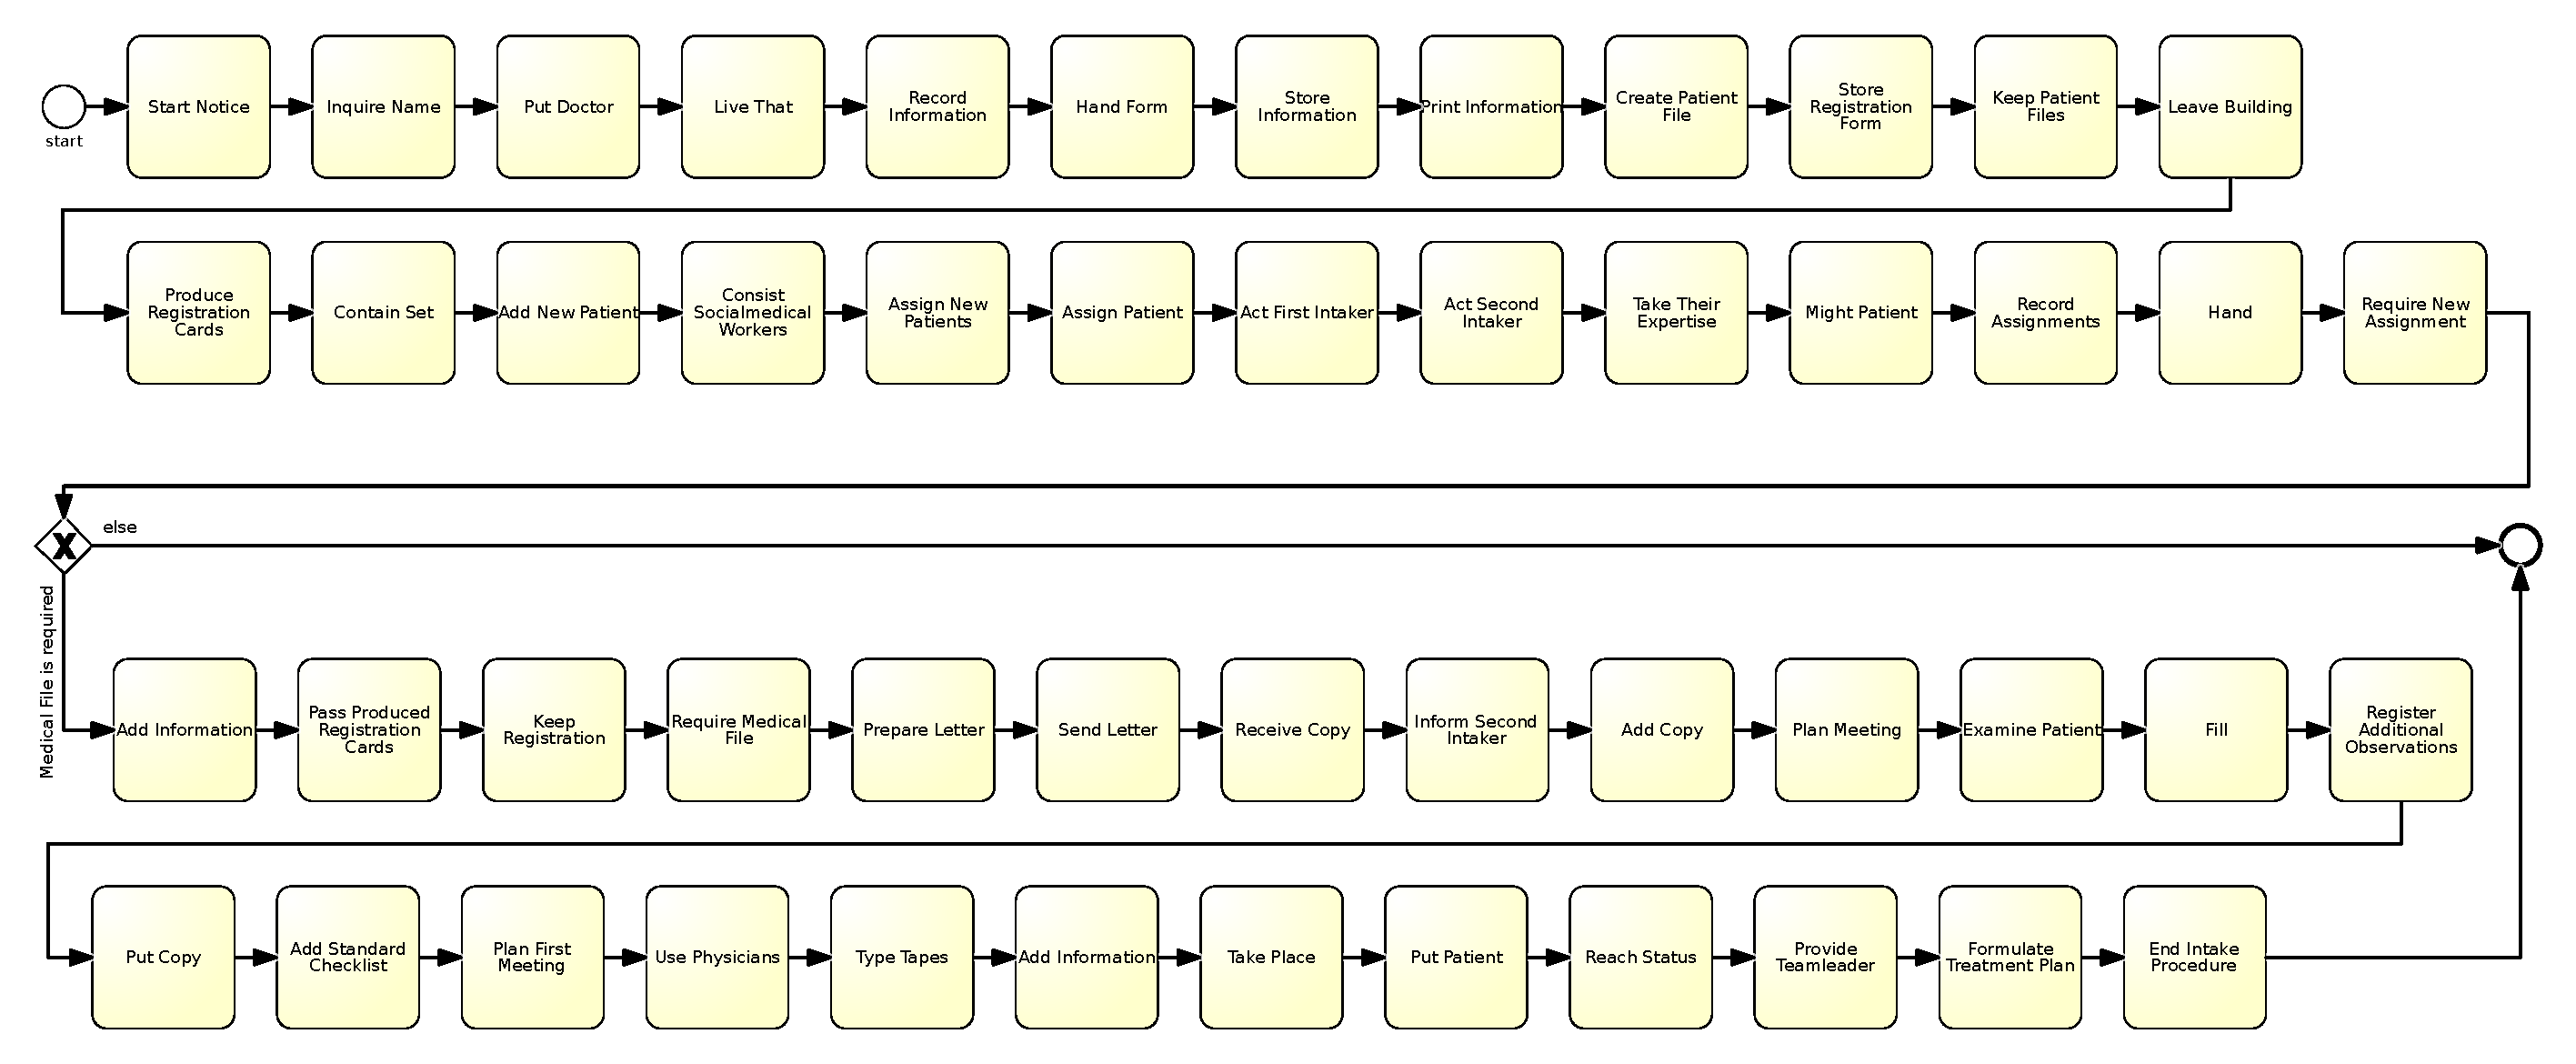
\includegraphics[width=0.95\textheight, angle=90]{./generated_bpmn/model14.pdf}
	\caption{BPMN diagram for process model 14 generated from spreadsheet-based model}
	\label{bpmn:generated_model14}
\end{figure}

\begin{figure}[H]
	\centering
	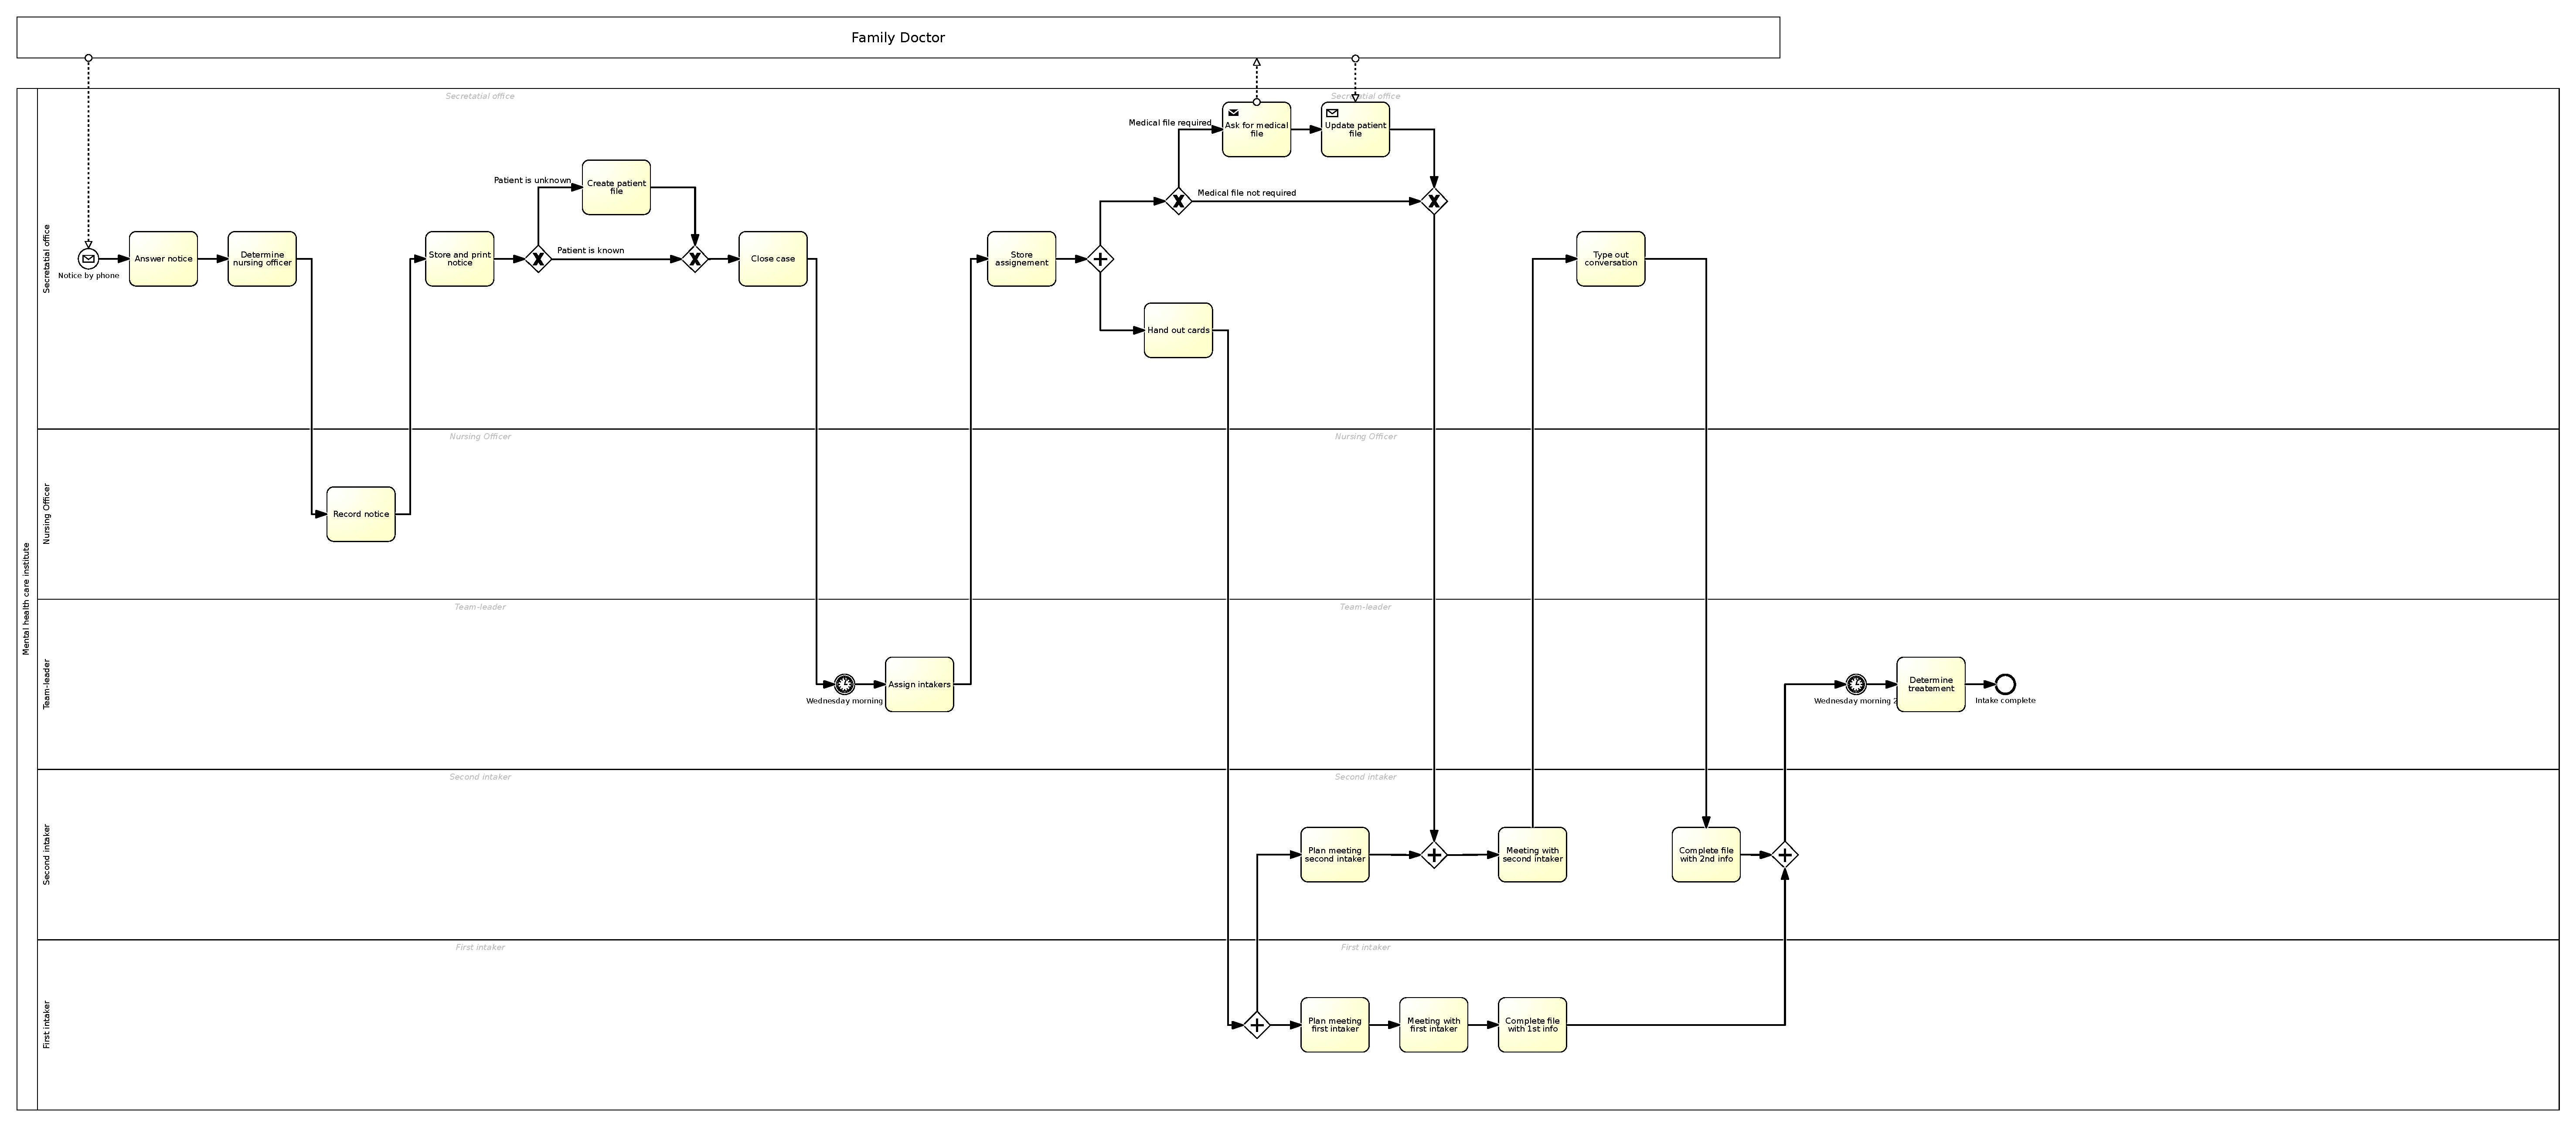
\includegraphics[width=0.95\textheight, angle=90]{./bpmn/model14.pdf}
	\caption{Hand-made BPMN diagram for process model 14}
	\label{bpmn:model14}
\end{figure}

\section{Model 15}
\begin{tcolorbox}[
	breakable,
	arc=0mm,
	left=1pt,
	right = 1pt,
	boxrule=0mm,
	colback = {white},
	]
	\texttt{\input{./models/model15.txt}}
\end{tcolorbox}
\captionof{textdesc}{Text description for model 15}
\label{txt:model15}

{\scriptsize
	\begin{longtable}{|p{0.03 \hsize}|p{0.25 \hsize}|p{0.15 \hsize}|p{0.2 \hsize}|p{0.1 \hsize}|p{0.1 \hsize}|}
		\hline
		Order & Activity & Condition & Who & Subprocess & Terminated.
		\\\hline\hline
		\csvreader[late after line=\\\hline]
		{./results/model15_intermediate_model.csv}
		{Order=\Order,Activity=\Activity,Condition=\Condition,Who=\Who,Subprocess=\Subprocess,Terminated=\Terminated}
		{\Order & \Activity & \Condition & \Who & \Subprocess & \Terminated}
		\caption{Spreadsheet-based description for process model 15}
		\label{csv:model15}
	\end{longtable}
}

\begin{figure}[H]
	\centering
	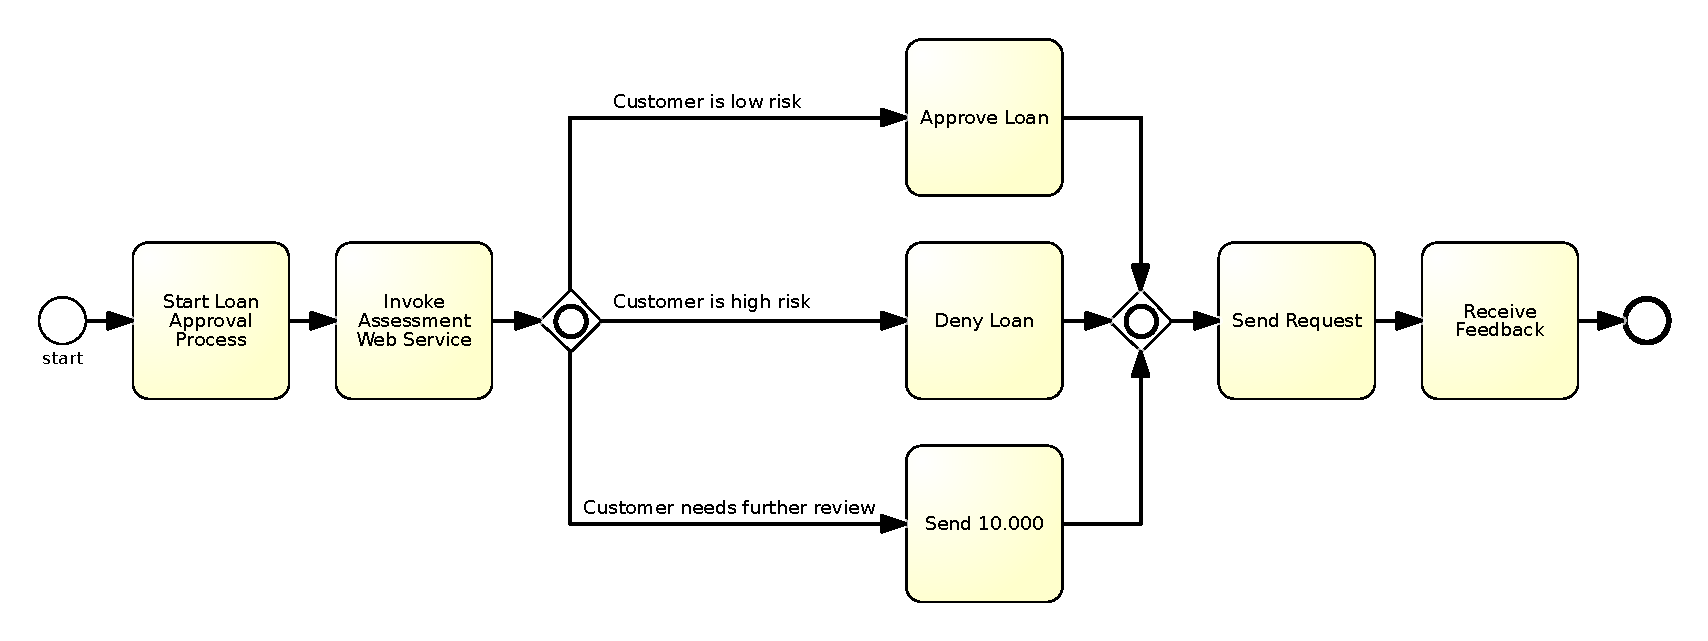
\includegraphics[width=\hsize]{./generated_bpmn/model15.pdf}
	\caption{BPMN diagram for process model 15 generated from spreadsheet-based model}
	\label{bpmn:generated_model15}
\end{figure}

\begin{figure}[H]
	\centering
	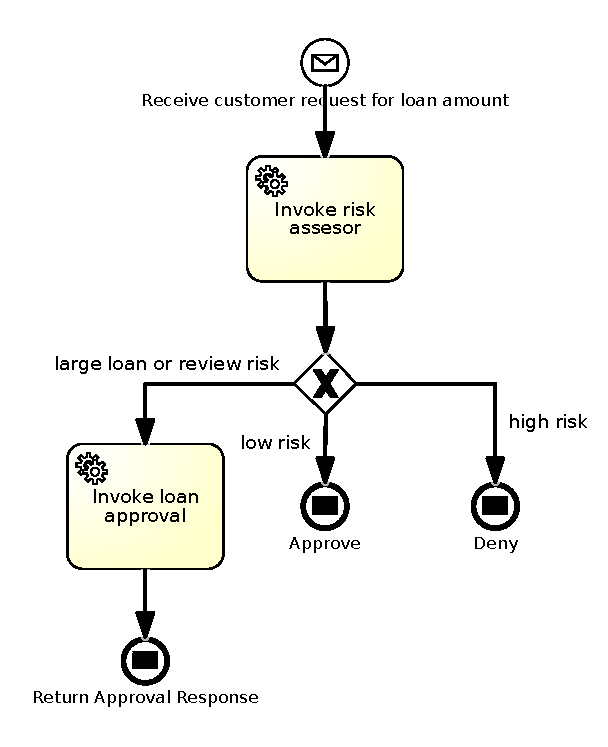
\includegraphics[scale=1.0]{./bpmn/model15.pdf}
	\caption{Hand-made BPMN diagram for process model 15}
	\label{bpmn:model15}
\end{figure}

\section{Model 16}
\begin{tcolorbox}[
	breakable,
	arc=0mm,
	left=1pt,
	right = 1pt,
	boxrule=0mm,
	colback = {white},
	]
	\texttt{\input{./models/model16.txt}}
\end{tcolorbox}
\captionof{textdesc}{Text description for model 16}
\label{txt:model16}

{\scriptsize
	\begin{longtable}{|p{0.03 \hsize}|p{0.25 \hsize}|p{0.15 \hsize}|p{0.2 \hsize}|p{0.1 \hsize}|p{0.1 \hsize}|}
		\hline
		Order & Activity & Condition & Who & Subprocess & Terminated.
		\\\hline\hline
		\csvreader[late after line=\\\hline]
		{./results/model16_intermediate_model.csv}
		{Order=\Order,Activity=\Activity,Condition=\Condition,Who=\Who,Subprocess=\Subprocess,Terminated=\Terminated}
		{\Order & \Activity & \Condition & \Who & \Subprocess & \Terminated}
		\caption{Spreadsheet-based description for process model 16}
		\label{csv:model16}
	\end{longtable}
}

\begin{figure}[H]
	\centering
	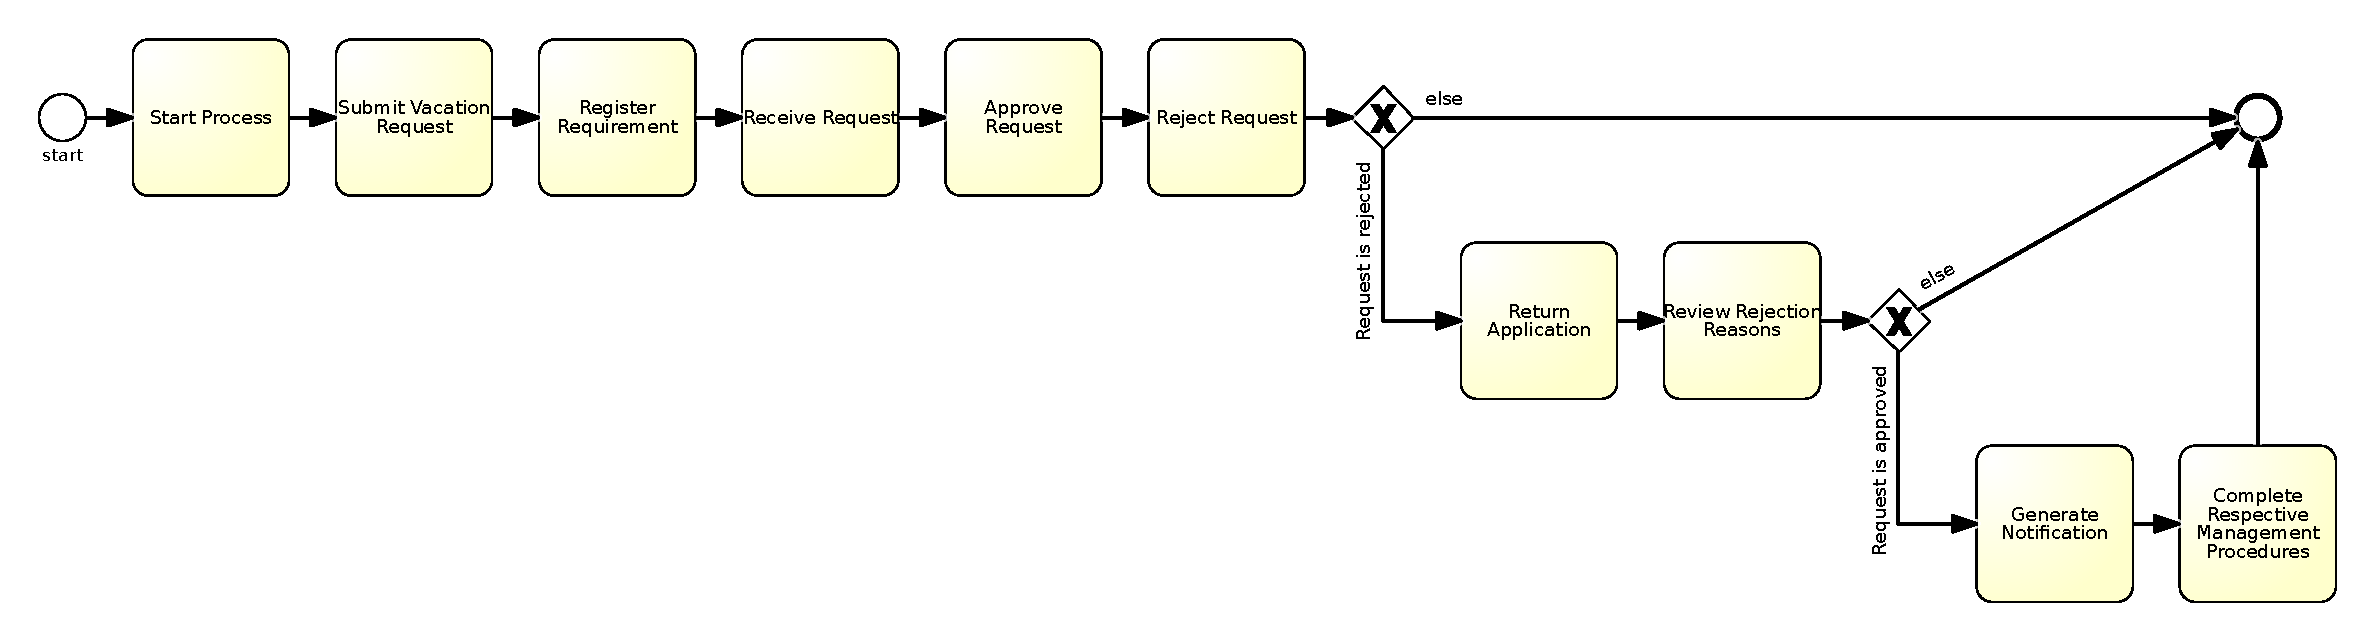
\includegraphics[width=\hsize]{./generated_bpmn/model16.pdf}
	\caption{BPMN diagram for process model 16 generated from spreadsheet-based model}
	\label{bpmn:generated_model16}
\end{figure}

\begin{figure}[H]
	\centering
	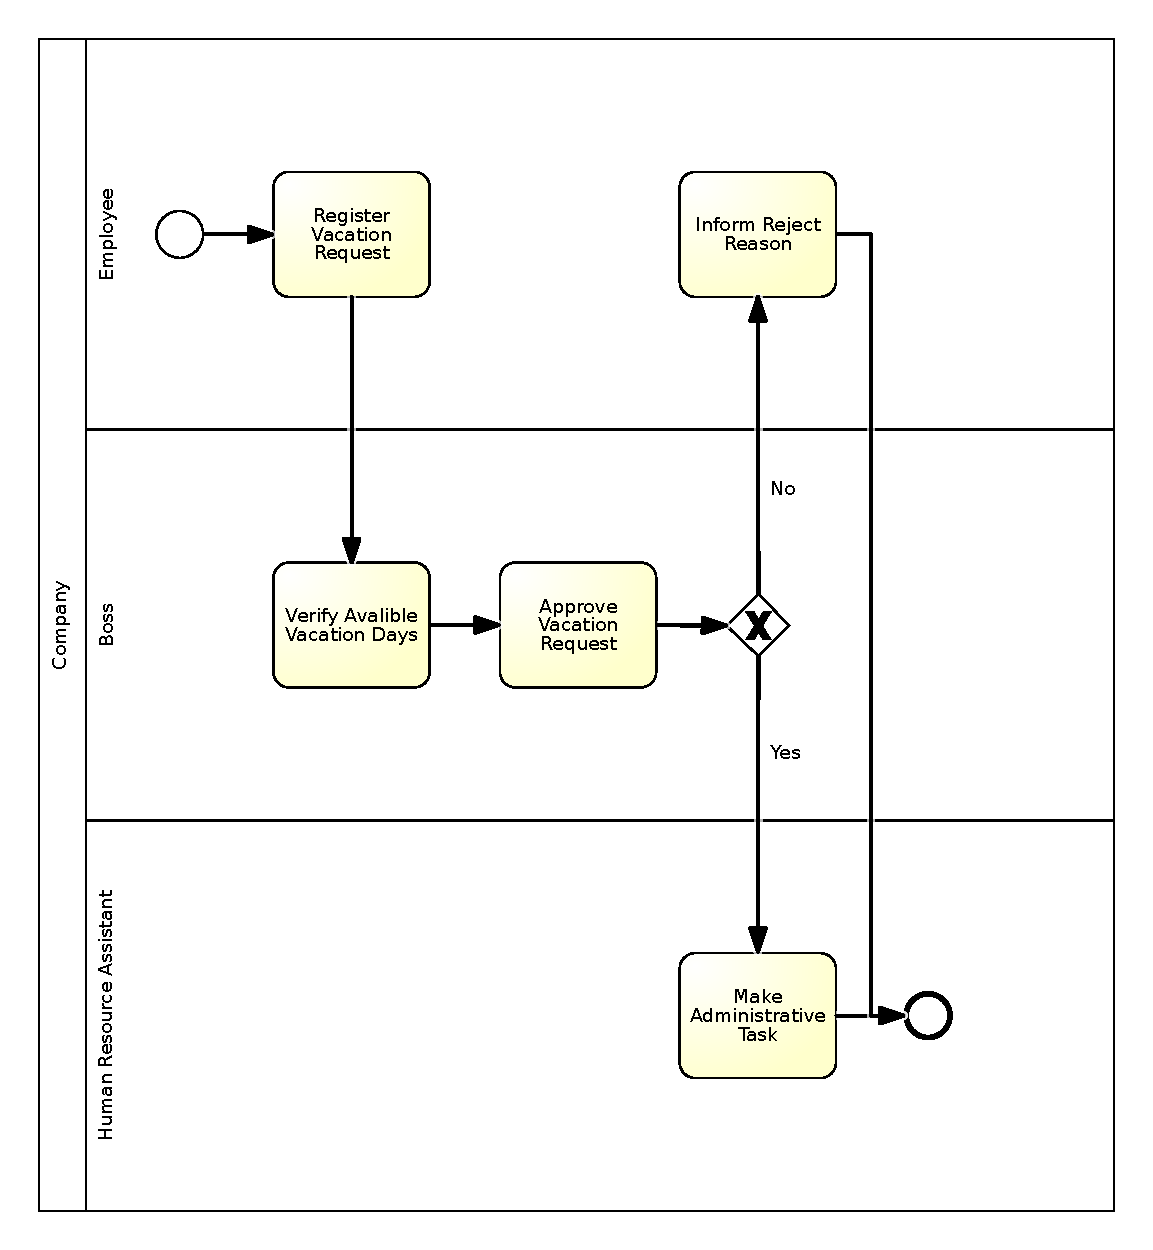
\includegraphics[scale=0.5]{./bpmn/model16.pdf}
	\caption{Hand-made BPMN diagram for process model 16}
	\label{bpmn:model16}
\end{figure}

\section{Model 17}
\begin{tcolorbox}[
	breakable,
	arc=0mm,
	left=1pt,
	right = 1pt,
	boxrule=0mm,
	colback = {white},
	]
	\texttt{\input{./models/model17.txt}}
\end{tcolorbox}
\captionof{textdesc}{Text description for model 17}
\label{txt:model17}

{\scriptsize
	\begin{longtable}{|p{0.03 \hsize}|p{0.25 \hsize}|p{0.15 \hsize}|p{0.2 \hsize}|p{0.1 \hsize}|p{0.1 \hsize}|}
		\hline
		Order & Activity & Condition & Who & Subprocess & Terminated.
		\\\hline\hline
		\csvreader[late after line=\\\hline]
		{./results/model17_intermediate_model.csv}
		{Order=\Order,Activity=\Activity,Condition=\Condition,Who=\Who,Subprocess=\Subprocess,Terminated=\Terminated}
		{\Order & \Activity & \Condition & \Who & \Subprocess & \Terminated}
		\caption{Spreadsheet-based description for process model 17}
		\label{csv:model17}
	\end{longtable}
}

\begin{figure}[H]
	\centering
	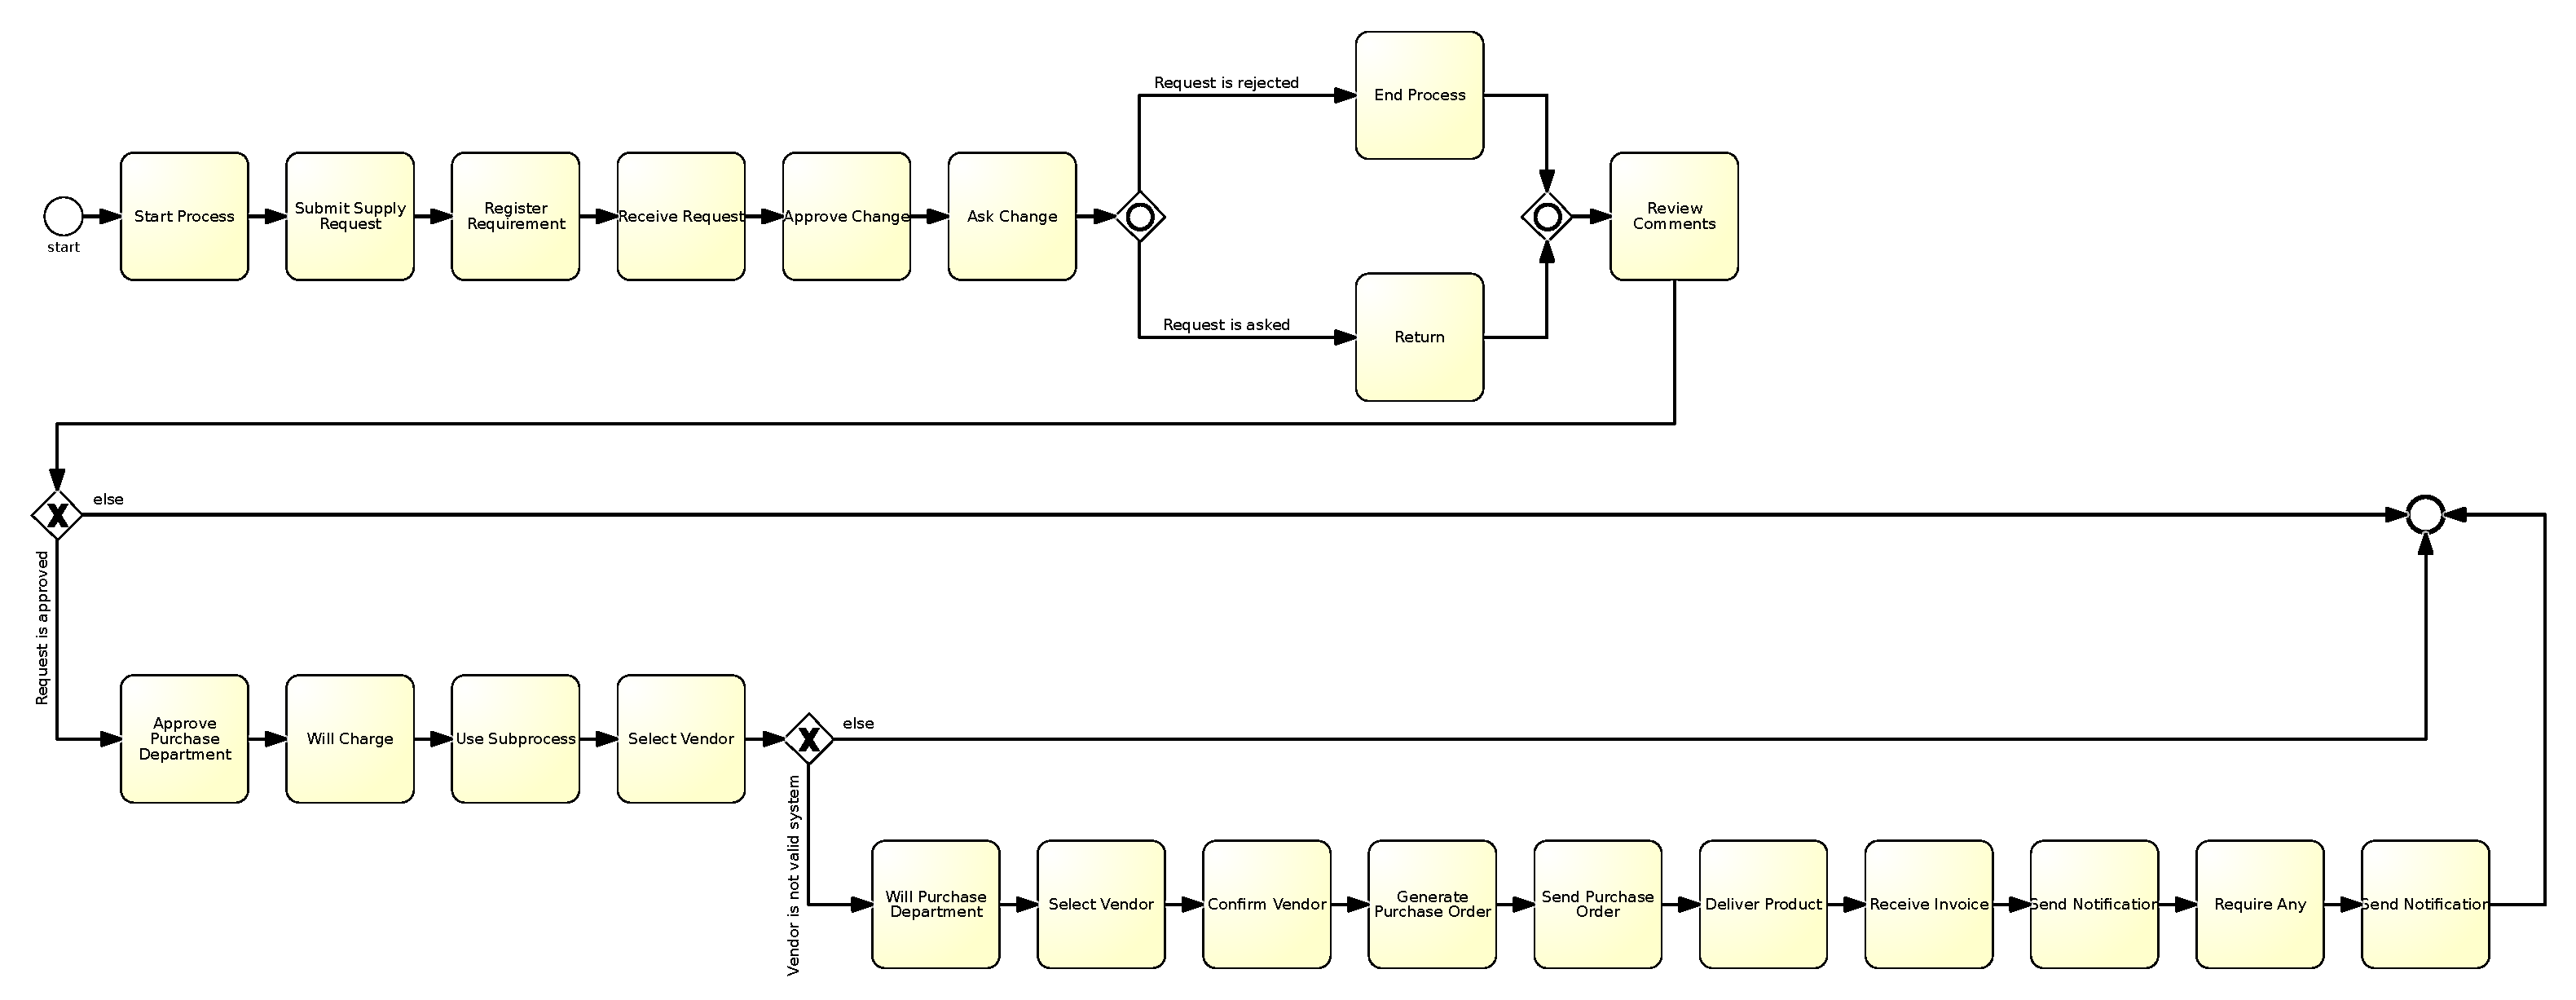
\includegraphics[width=\hsize]{./generated_bpmn/model17.pdf}
	\caption{BPMN diagram for process model 17 generated from spreadsheet-based model}
	\label{bpmn:generated_model17}
\end{figure}

\begin{figure}[H]
	\centering
	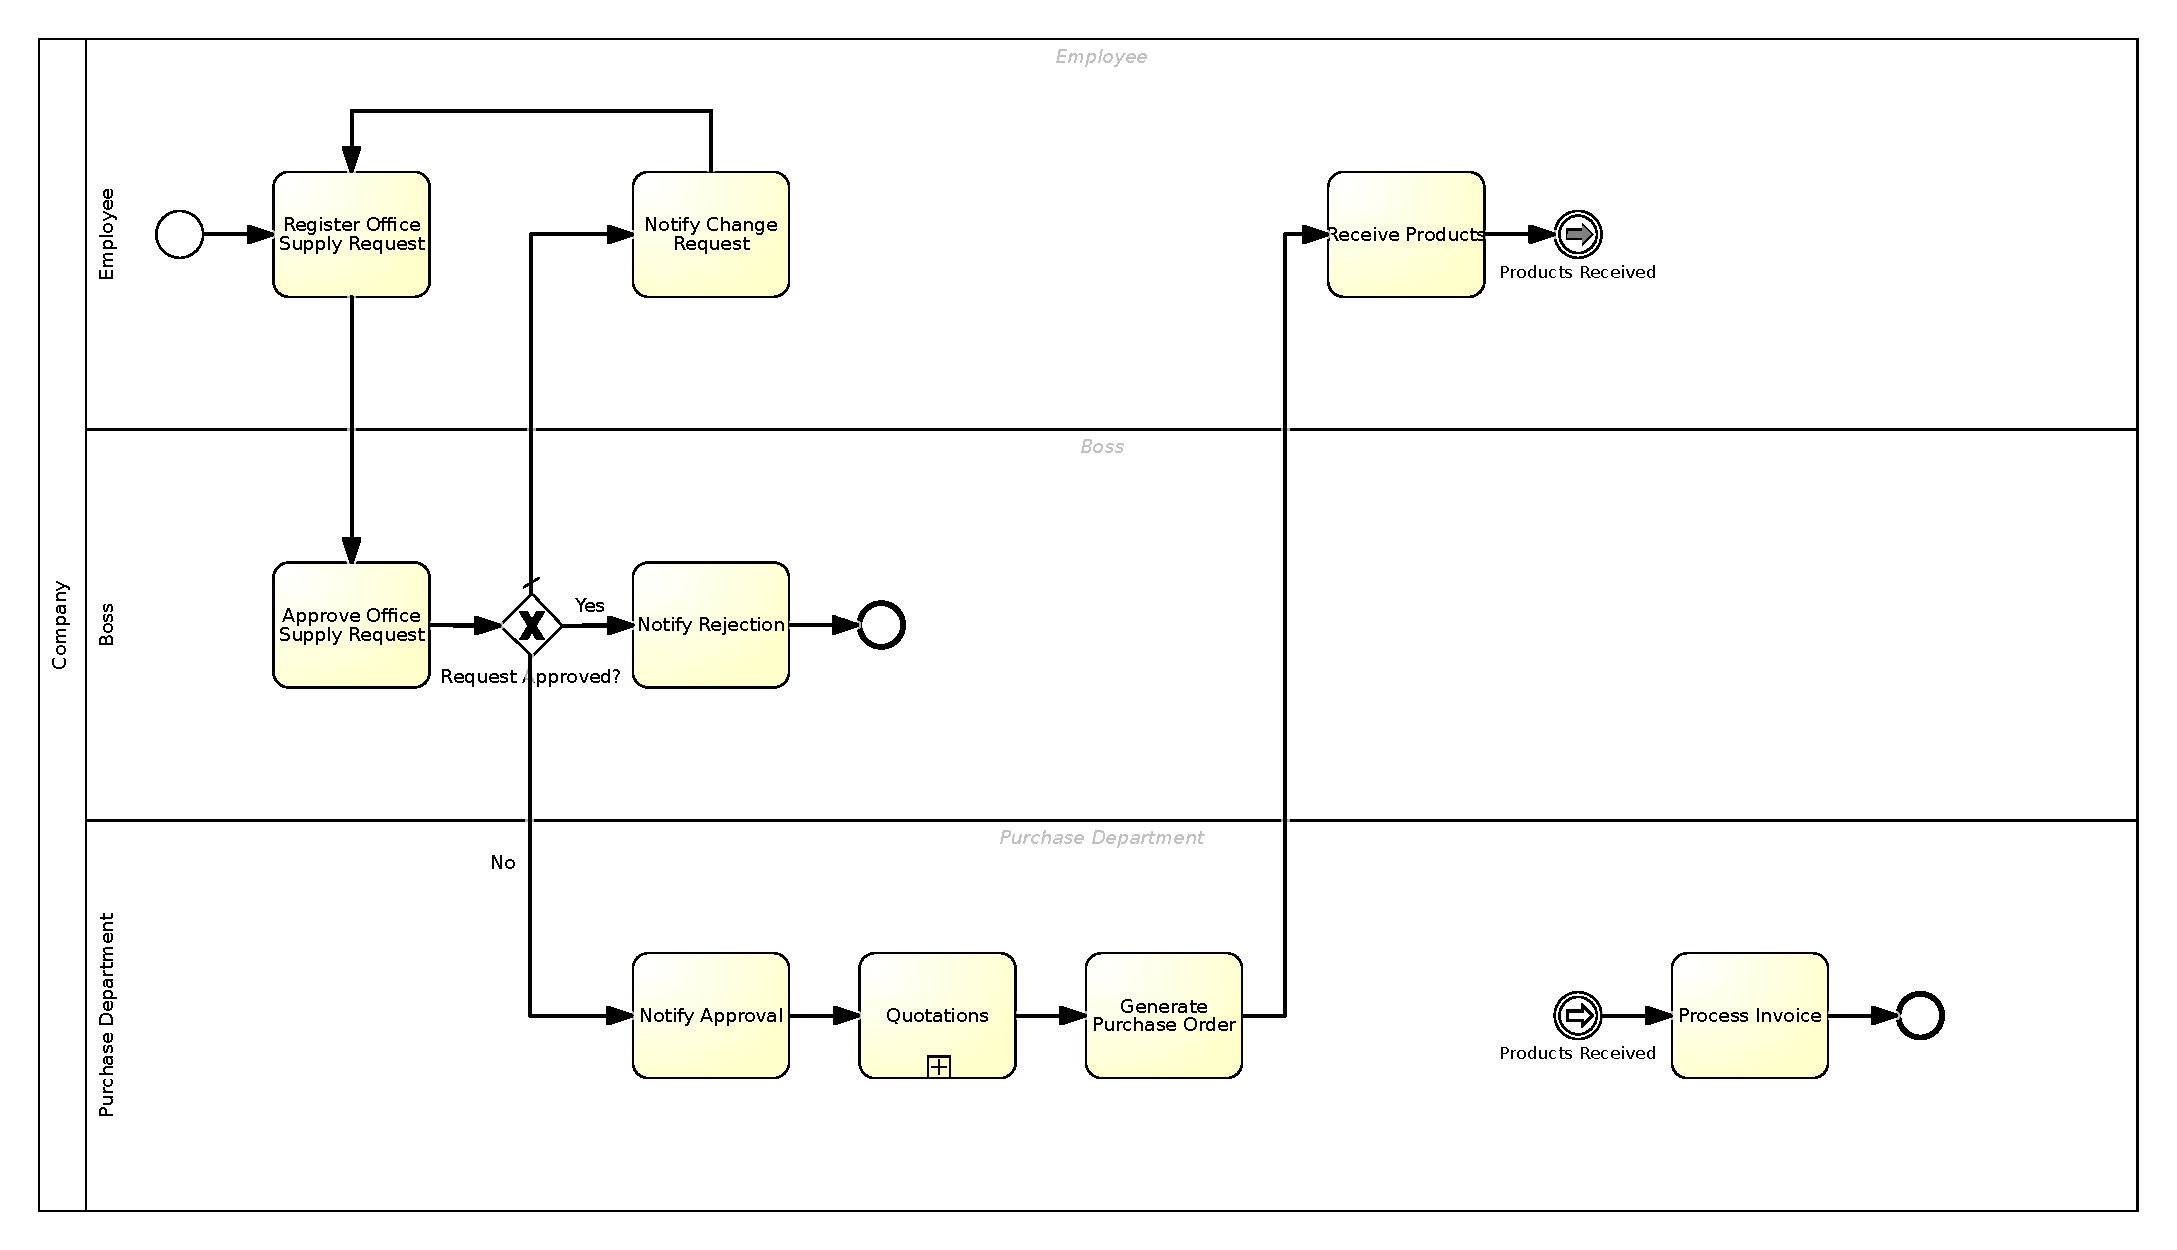
\includegraphics[width=\hsize]{./bpmn/model17.pdf}
	\caption{Hand-made BPMN diagram for process model 17}
	\label{bpmn:model17}
\end{figure}

\section{Model 18}
\begin{tcolorbox}[
	breakable,
	arc=0mm,
	left=1pt,
	right = 1pt,
	boxrule=0mm,
	colback = {white},
	]
	\texttt{\input{./models/model18.txt}}
\end{tcolorbox}
\captionof{textdesc}{Text description for model 18}
\label{txt:model18}

{\scriptsize
	\begin{longtable}{|p{0.03 \hsize}|p{0.25 \hsize}|p{0.15 \hsize}|p{0.2 \hsize}|p{0.1 \hsize}|p{0.1 \hsize}|}
		\hline
		Order & Activity & Condition & Who & Subprocess & Terminated.
		\\\hline\hline
		\csvreader[late after line=\\\hline]
		{./results/model18_intermediate_model.csv}
		{Order=\Order,Activity=\Activity,Condition=\Condition,Who=\Who,Subprocess=\Subprocess,Terminated=\Terminated}
		{\Order & \Activity & \Condition & \Who & \Subprocess & \Terminated}
		\caption{Spreadsheet-based description for process model 18}
		\label{csv:model18}
	\end{longtable}
}

\begin{figure}[H]
	\centering
	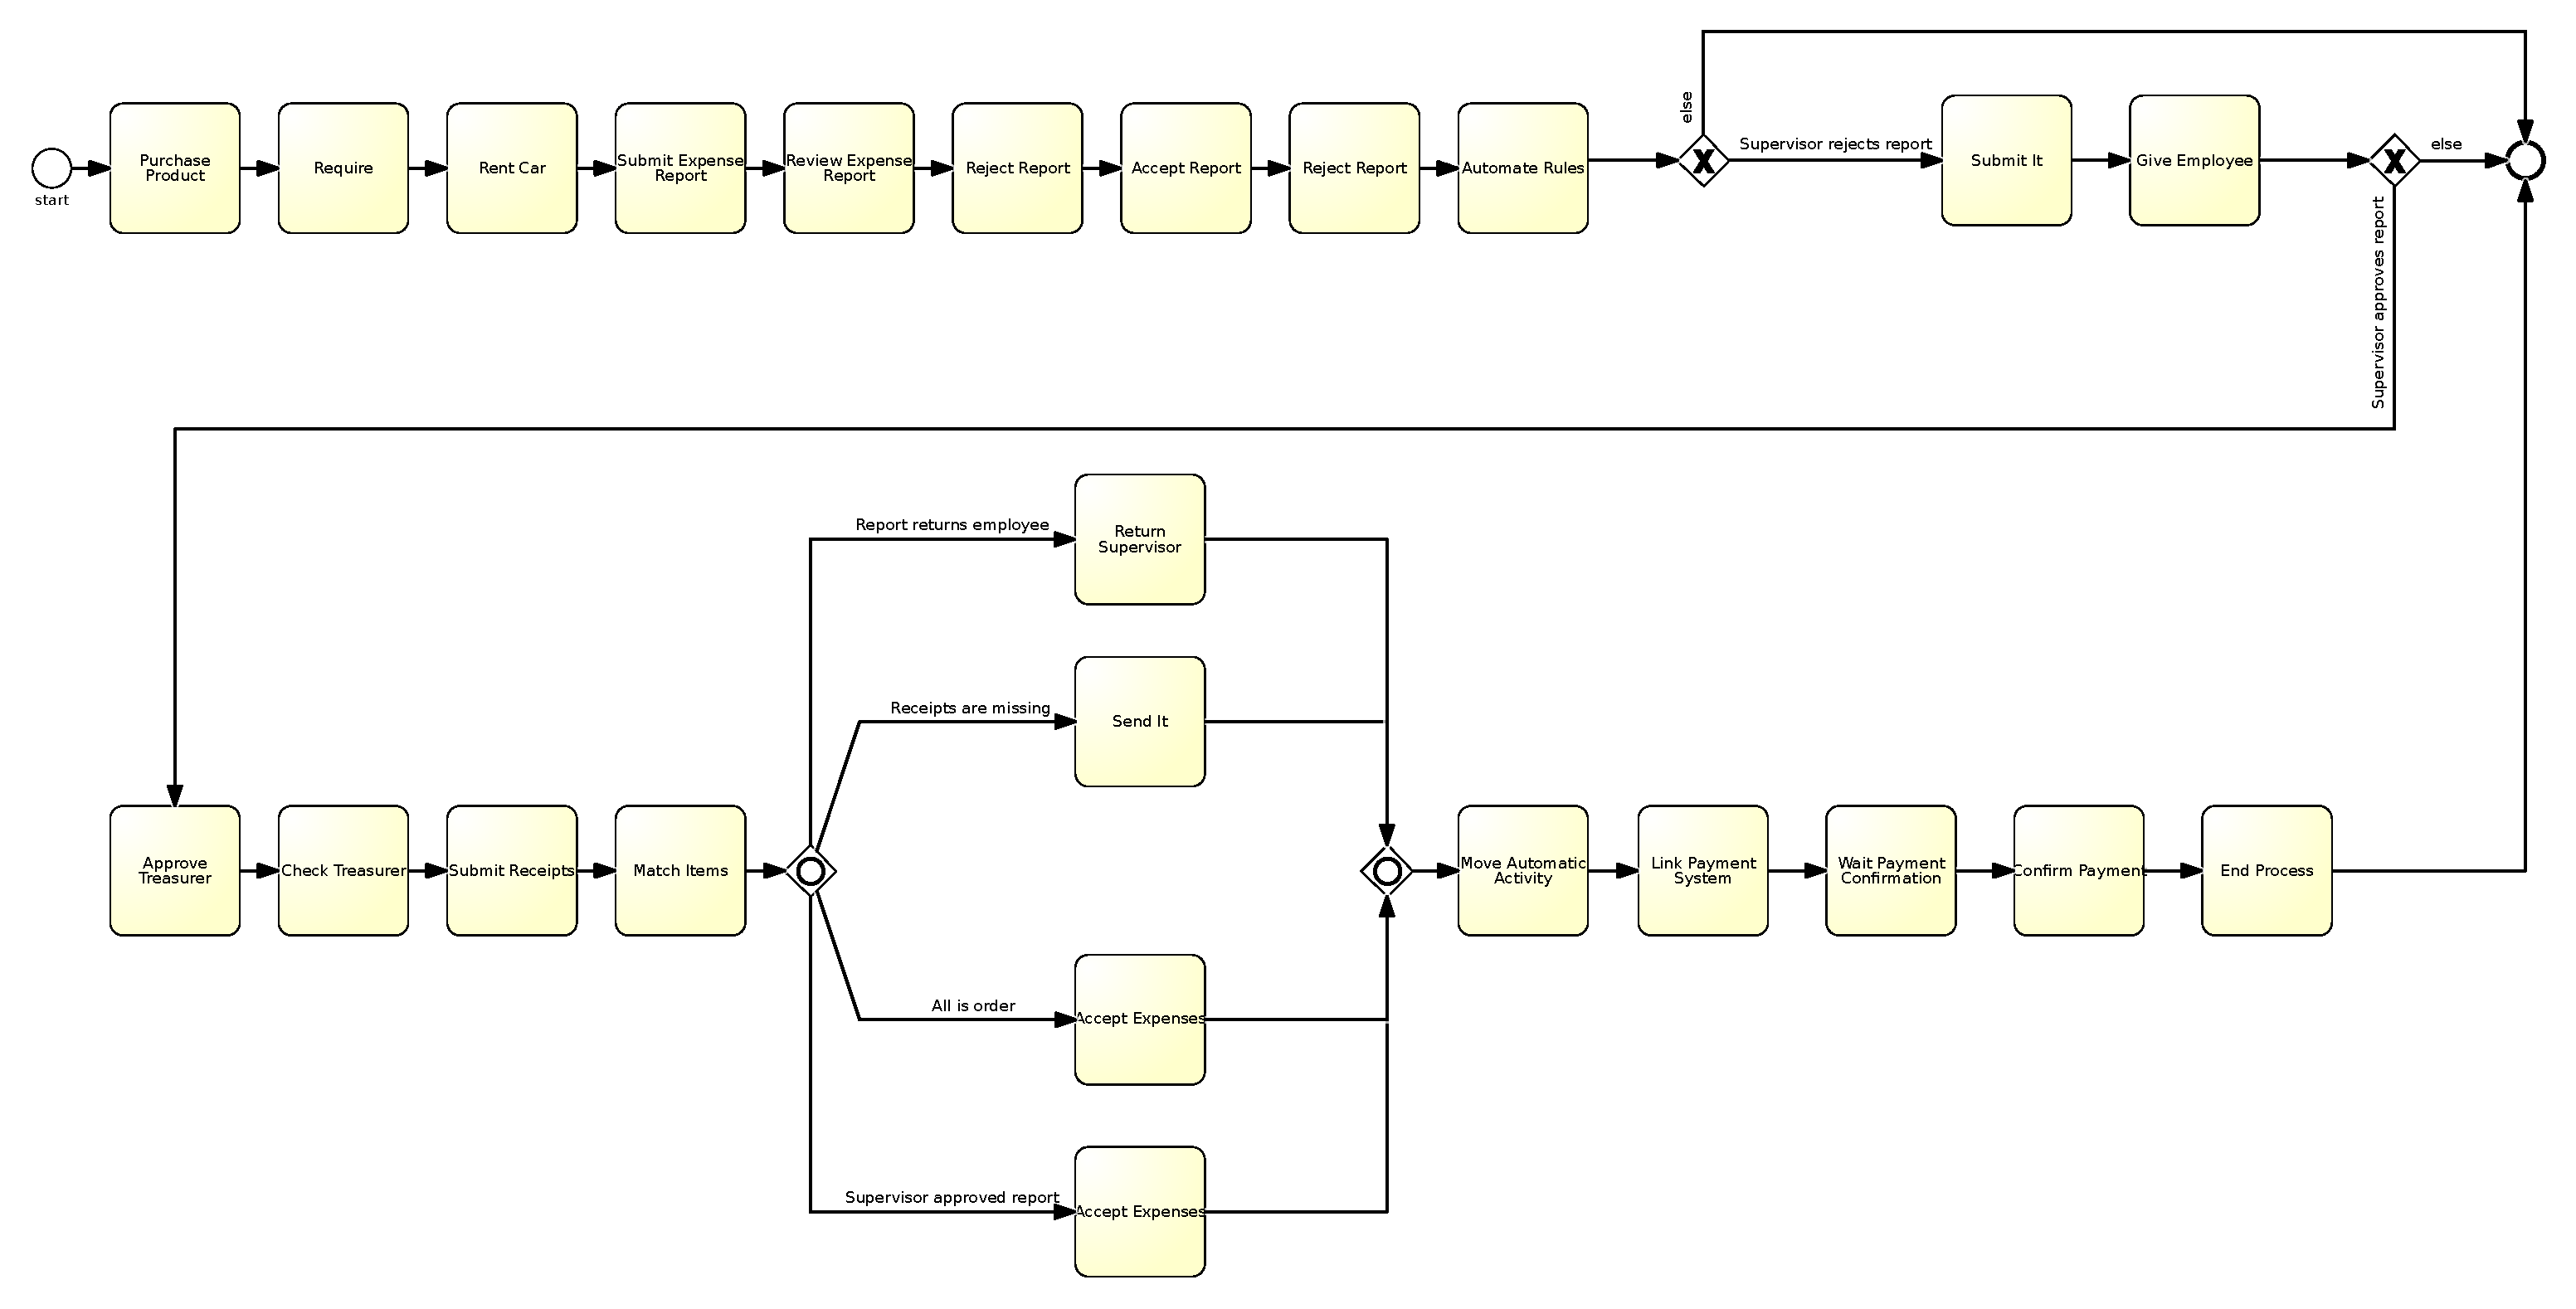
\includegraphics[width=\hsize]{./generated_bpmn/model18.pdf}
	\caption{BPMN diagram for process model 18 generated from spreadsheet-based model}
	\label{bpmn:generated_model18}
\end{figure}

\begin{figure}[H]
	\centering
	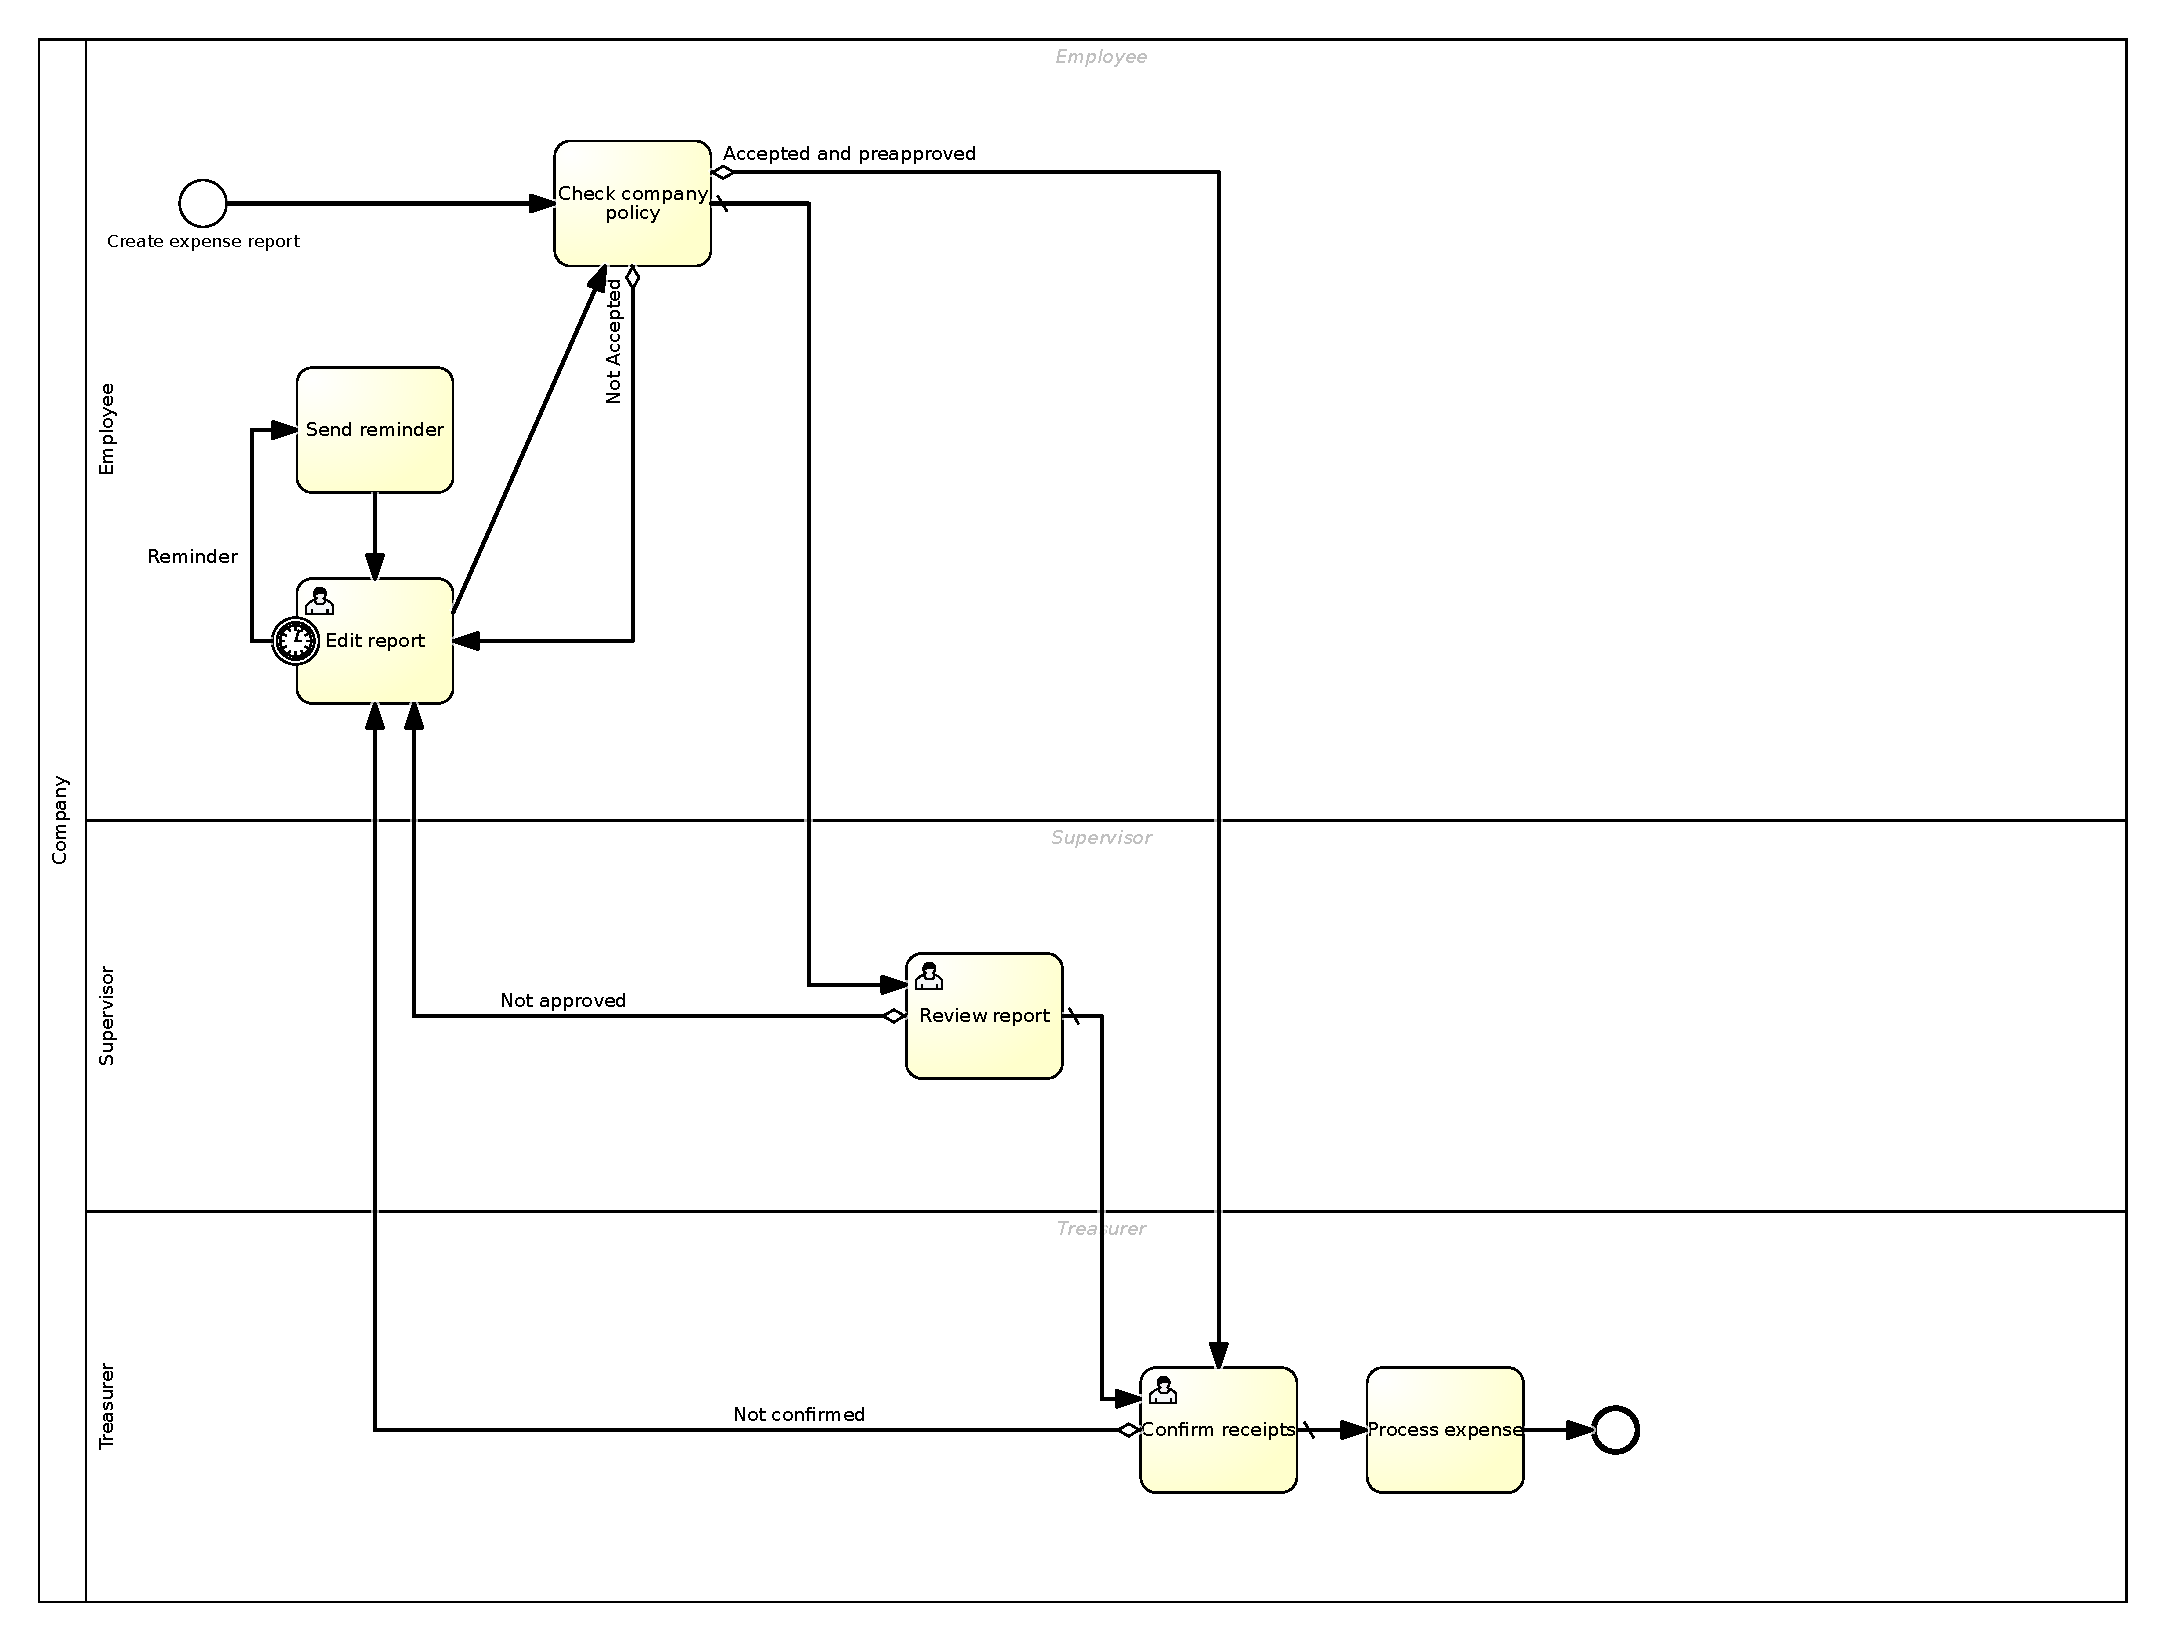
\includegraphics[width=\hsize]{./bpmn/model18.pdf}
	\caption{Hand-made BPMN diagram for process model 18}
	\label{bpmn:model18}
\end{figure}

\section{Model 19}
\begin{tcolorbox}[
	breakable,
	arc=0mm,
	left=1pt,
	right = 1pt,
	boxrule=0mm,
	colback = {white},
	]
	\texttt{\input{./models/model19.txt}}
\end{tcolorbox}
\captionof{textdesc}{Text description for model 19}
\label{txt:model19}
\newpage
{\scriptsize
	\begin{longtable}{|p{0.03 \hsize}|p{0.25 \hsize}|p{0.15 \hsize}|p{0.2 \hsize}|p{0.1 \hsize}|p{0.1 \hsize}|}
		\hline
		Order & Activity & Condition & Who & Subprocess & Terminated.
		\\\hline\hline
		\csvreader[late after line=\\\hline]
		{./results/model19_intermediate_model.csv}
		{Order=\Order,Activity=\Activity,Condition=\Condition,Who=\Who,Subprocess=\Subprocess,Terminated=\Terminated}
		{\Order & \Activity & \Condition & \Who & \Subprocess & \Terminated}
		\caption{Spreadsheet-based description for process model 19}
		\label{csv:model19}
	\end{longtable}
}

\begin{figure}[H]
	\centering
	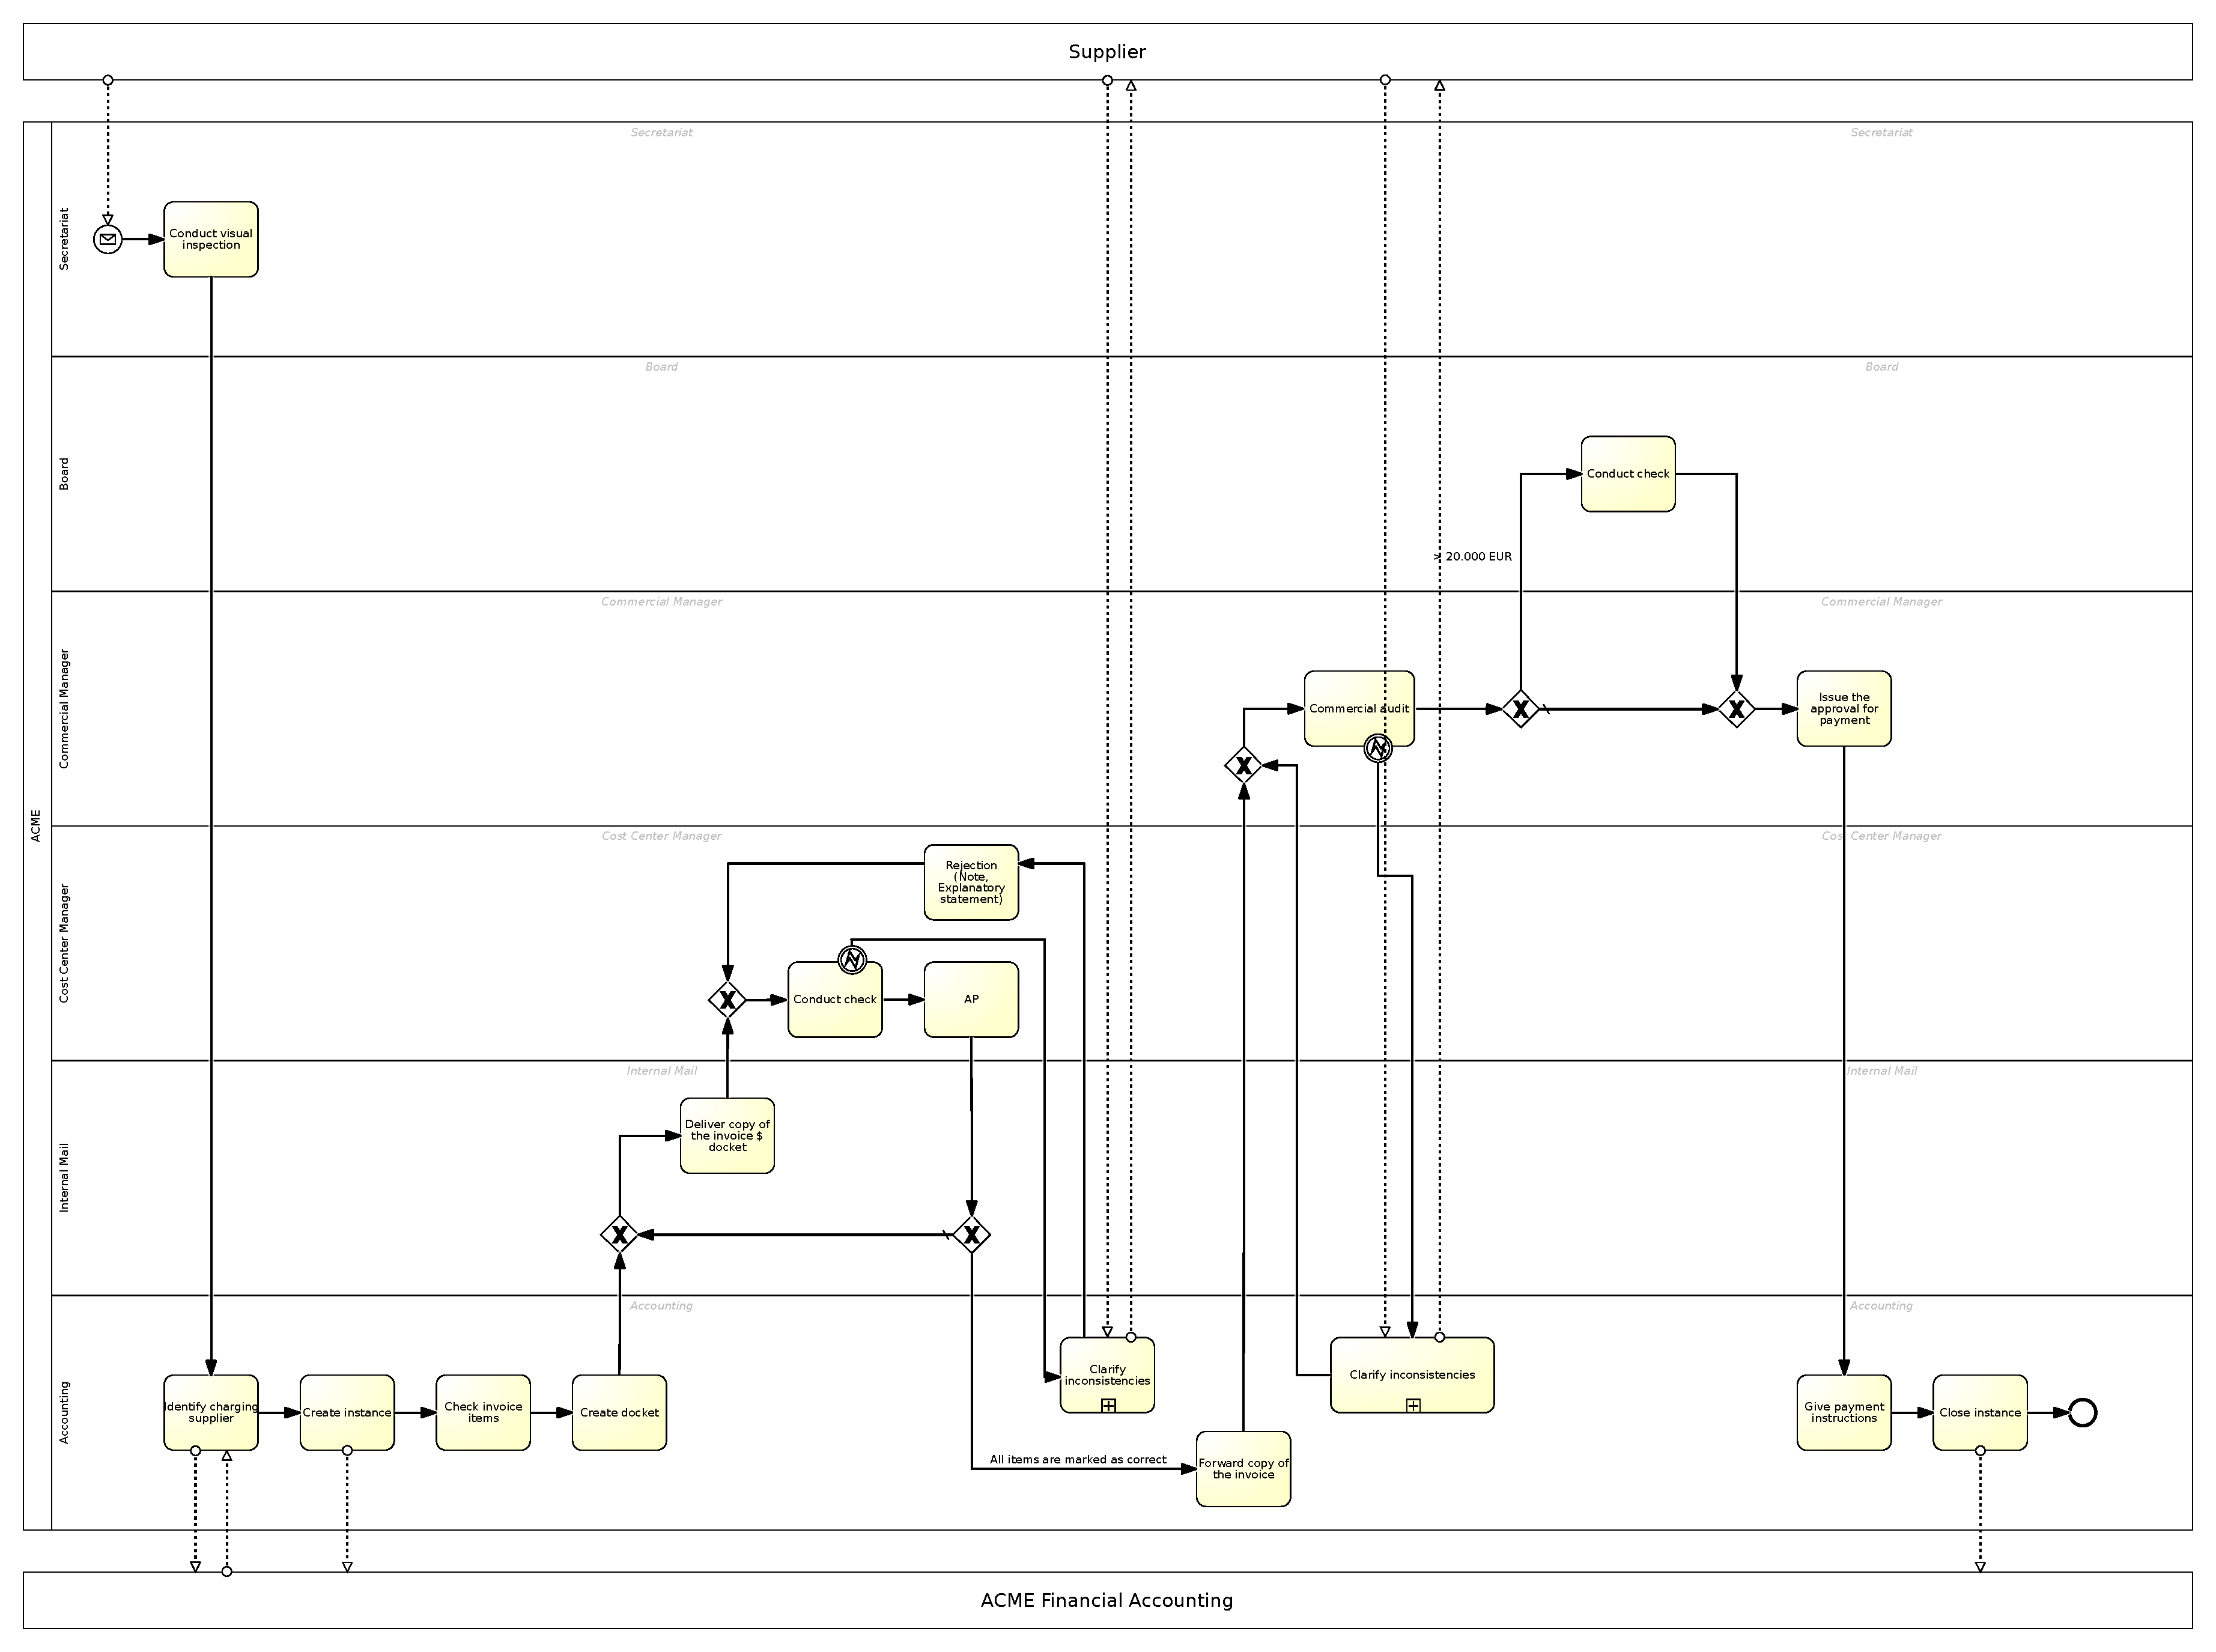
\includegraphics[width=\hsize]{./bpmn/model19.pdf}
	\caption{Hand-made BPMN diagram for process model 19}
	\label{bpmn:model19}
\end{figure}

\begin{figure}[H]
	\centering
	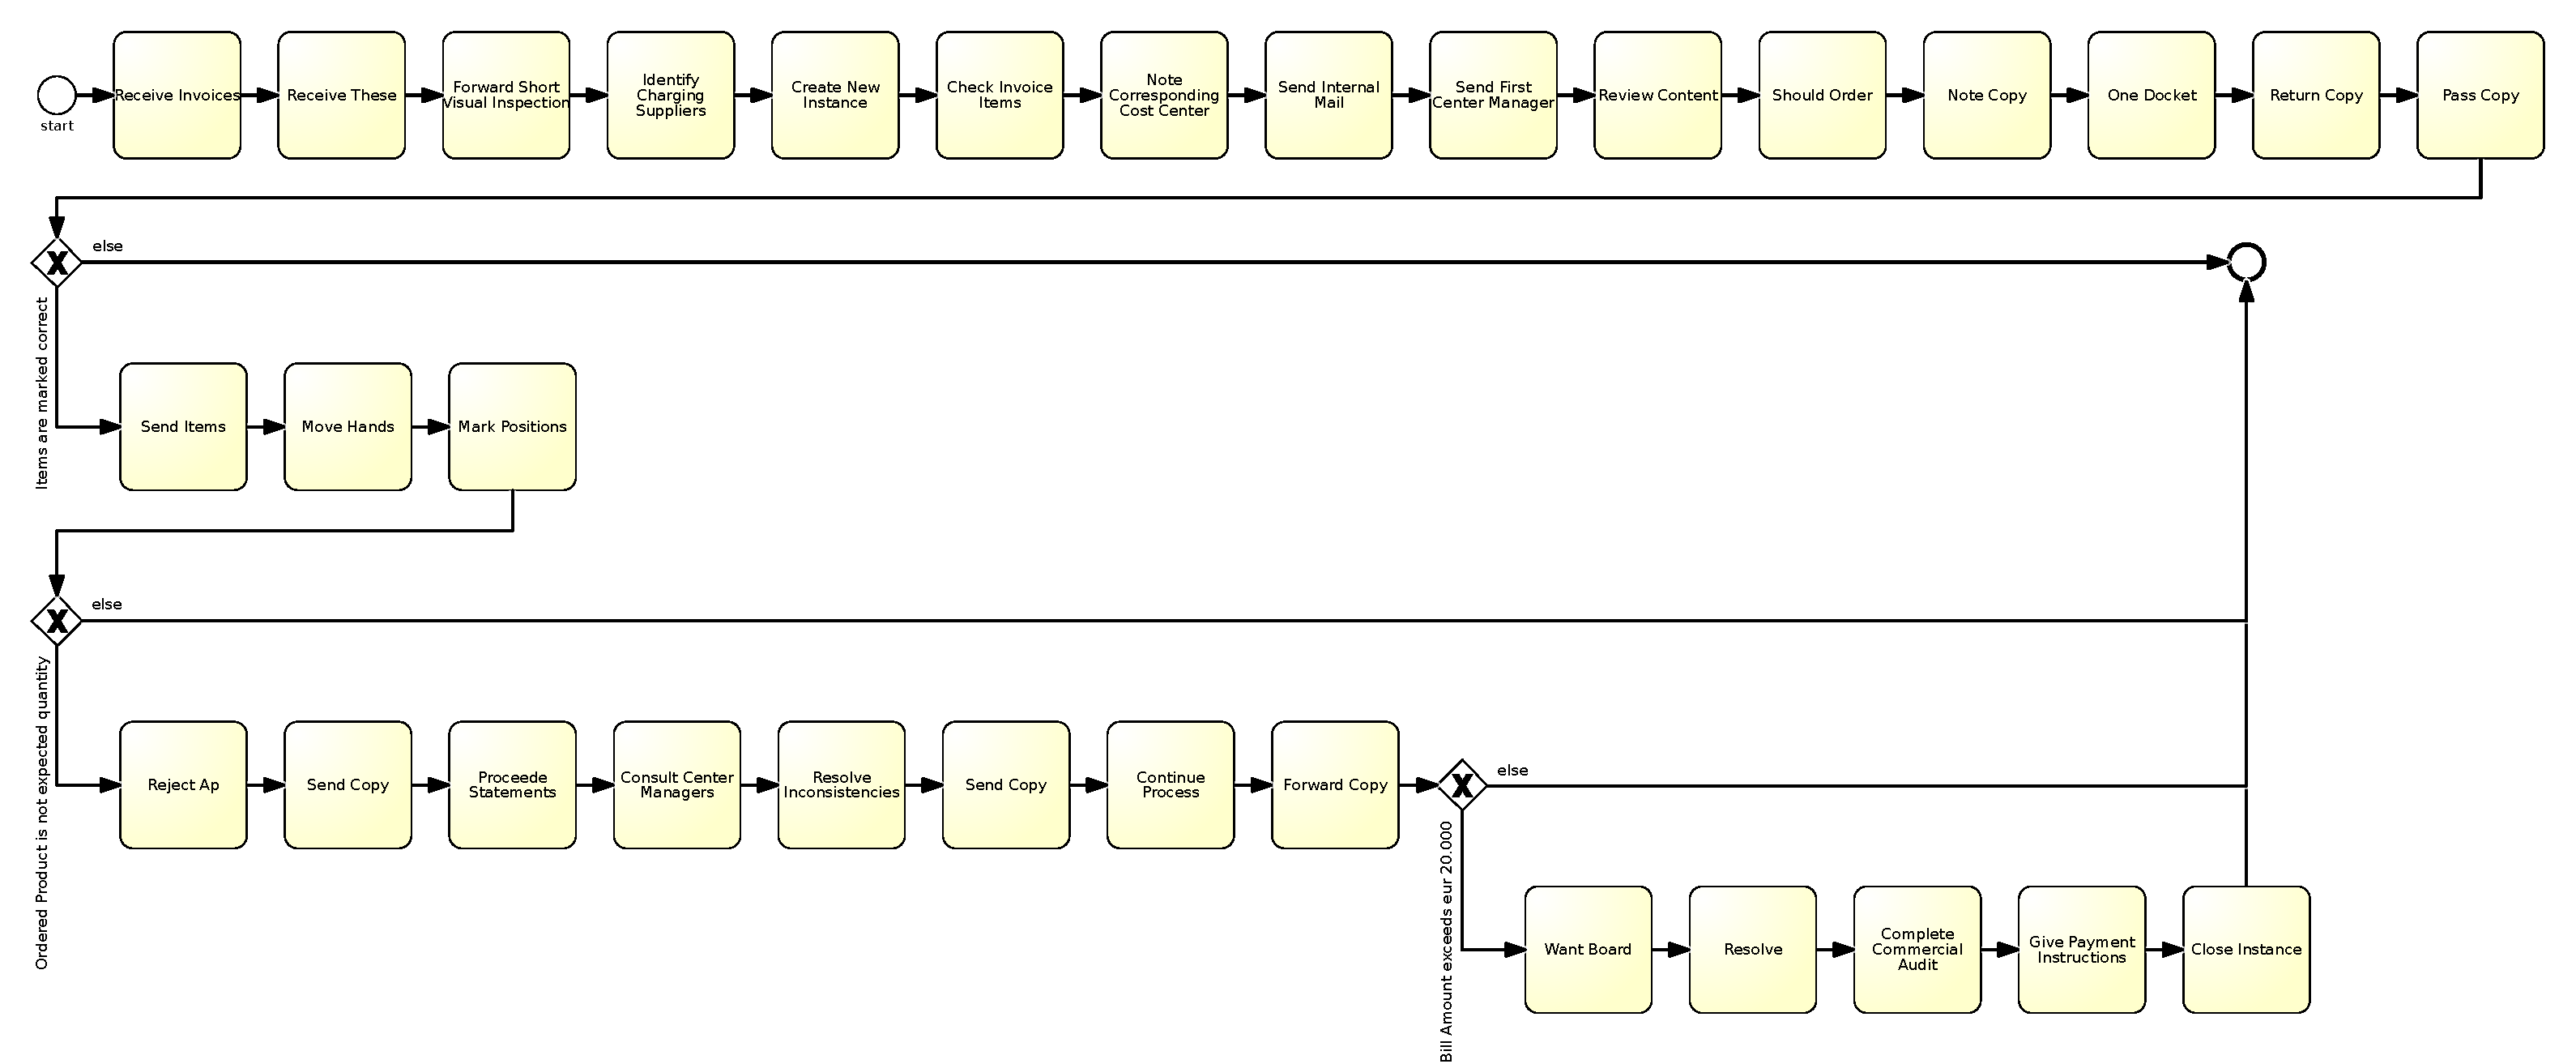
\includegraphics[width=\hsize]{./generated_bpmn/model19.pdf}
	\caption{BPMN diagram for process model 19 generated from spreadsheet-based model}
	\label{bpmn:generated_model19}
\end{figure}

\section{Model 20}
\begin{tcolorbox}[
	breakable,
	arc=0mm,
	left=1pt,
	right = 1pt,
	boxrule=0mm,
	colback = {white},
	]
	\texttt{\input{./models/model20.txt}}
\end{tcolorbox}
\captionof{textdesc}{Text description for model 20}
\label{txt:model20}

{\scriptsize
	\begin{longtable}{|p{0.03 \hsize}|p{0.25 \hsize}|p{0.15 \hsize}|p{0.2 \hsize}|p{0.1 \hsize}|p{0.1 \hsize}|}
		\hline
		Order & Activity & Condition & Who & Subprocess & Terminated.
		\\\hline\hline
		\csvreader[late after line=\\\hline]
		{./results/model20_intermediate_model.csv}
		{Order=\Order,Activity=\Activity,Condition=\Condition,Who=\Who,Subprocess=\Subprocess,Terminated=\Terminated}
		{\Order & \Activity & \Condition & \Who & \Subprocess & \Terminated}
		\caption{Spreadsheet-based description for process model 20}
		\label{csv:model20}
	\end{longtable}
}

\begin{figure}[H]
	\centering
	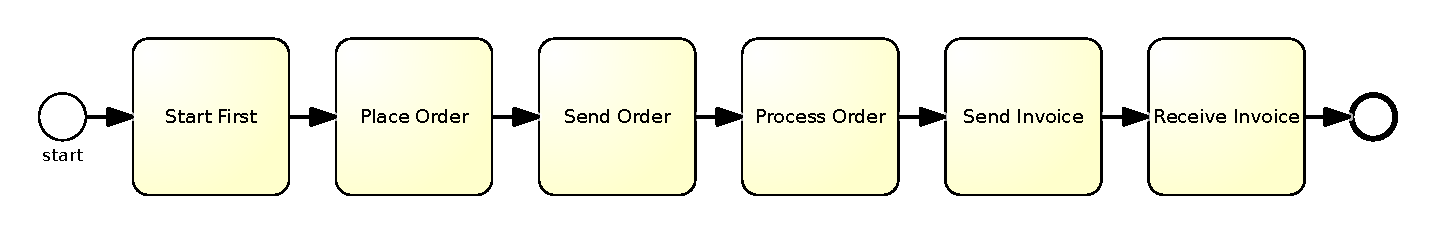
\includegraphics[width=\hsize]{./generated_bpmn/model20.pdf}
	\caption{BPMN diagram for process model 20 generated from spreadsheet-based model}
	\label{bpmn:generated_model20}
\end{figure}

\begin{figure}[H]
	\centering
	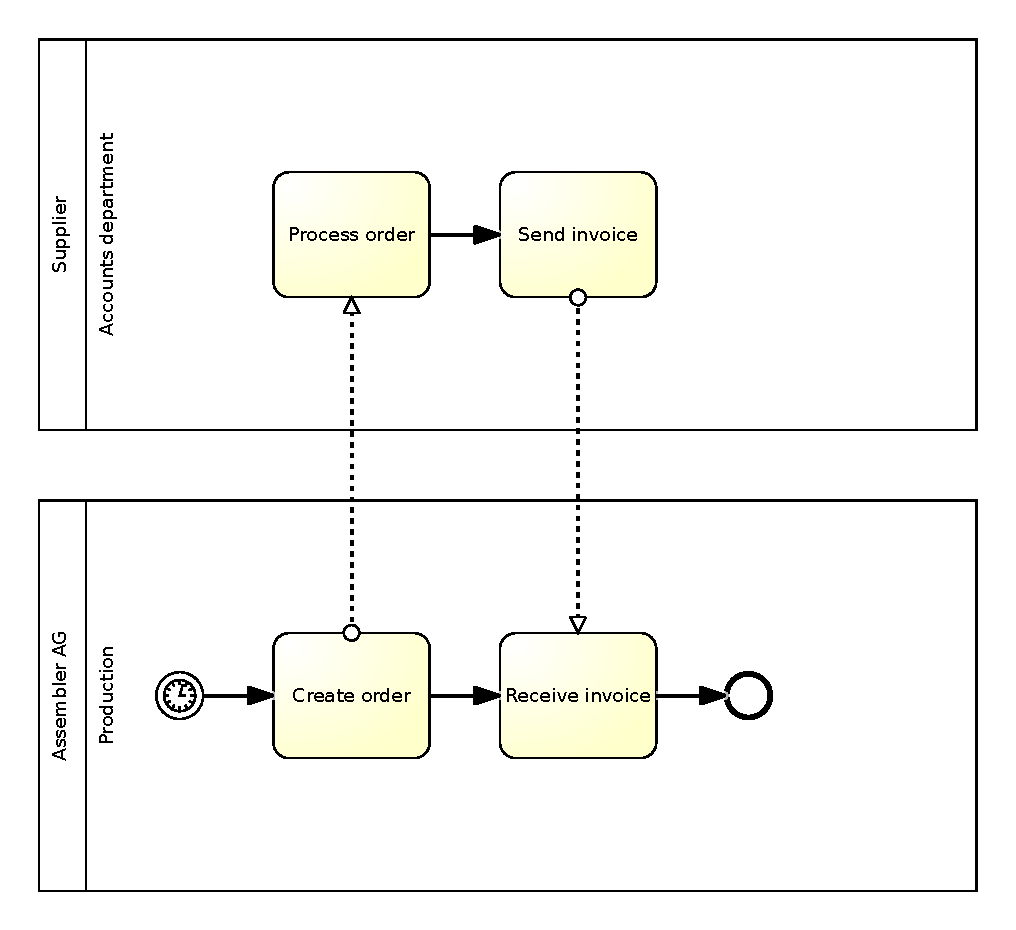
\includegraphics[scale=0.7]{./bpmn/model20.pdf}
	\caption{Hand-made BPMN diagram for process model 20}
	\label{bpmn:model20}
\end{figure}

\section{Model 21}
\begin{tcolorbox}[
	breakable,
	arc=0mm,
	left=1pt,
	right = 1pt,
	boxrule=0mm,
	colback = {white},
	]
	\texttt{\input{./models/model21.txt}}
\end{tcolorbox}
\captionof{textdesc}{Text description for model 21}
\label{txt:model21}

{\scriptsize
	\begin{longtable}{|p{0.03 \hsize}|p{0.25 \hsize}|p{0.15 \hsize}|p{0.2 \hsize}|p{0.1 \hsize}|p{0.1 \hsize}|}
		\hline
		Order & Activity & Condition & Who & Subprocess & Terminated.
		\\\hline\hline
		\csvreader[late after line=\\\hline]
		{./results/model21_intermediate_model.csv}
		{Order=\Order,Activity=\Activity,Condition=\Condition,Who=\Who,Subprocess=\Subprocess,Terminated=\Terminated}
		{\Order & \Activity & \Condition & \Who & \Subprocess & \Terminated}
		\caption{Spreadsheet-based description for process model 21}
		\label{csv:model21}
	\end{longtable}
}

\begin{figure}[H]
	\centering
	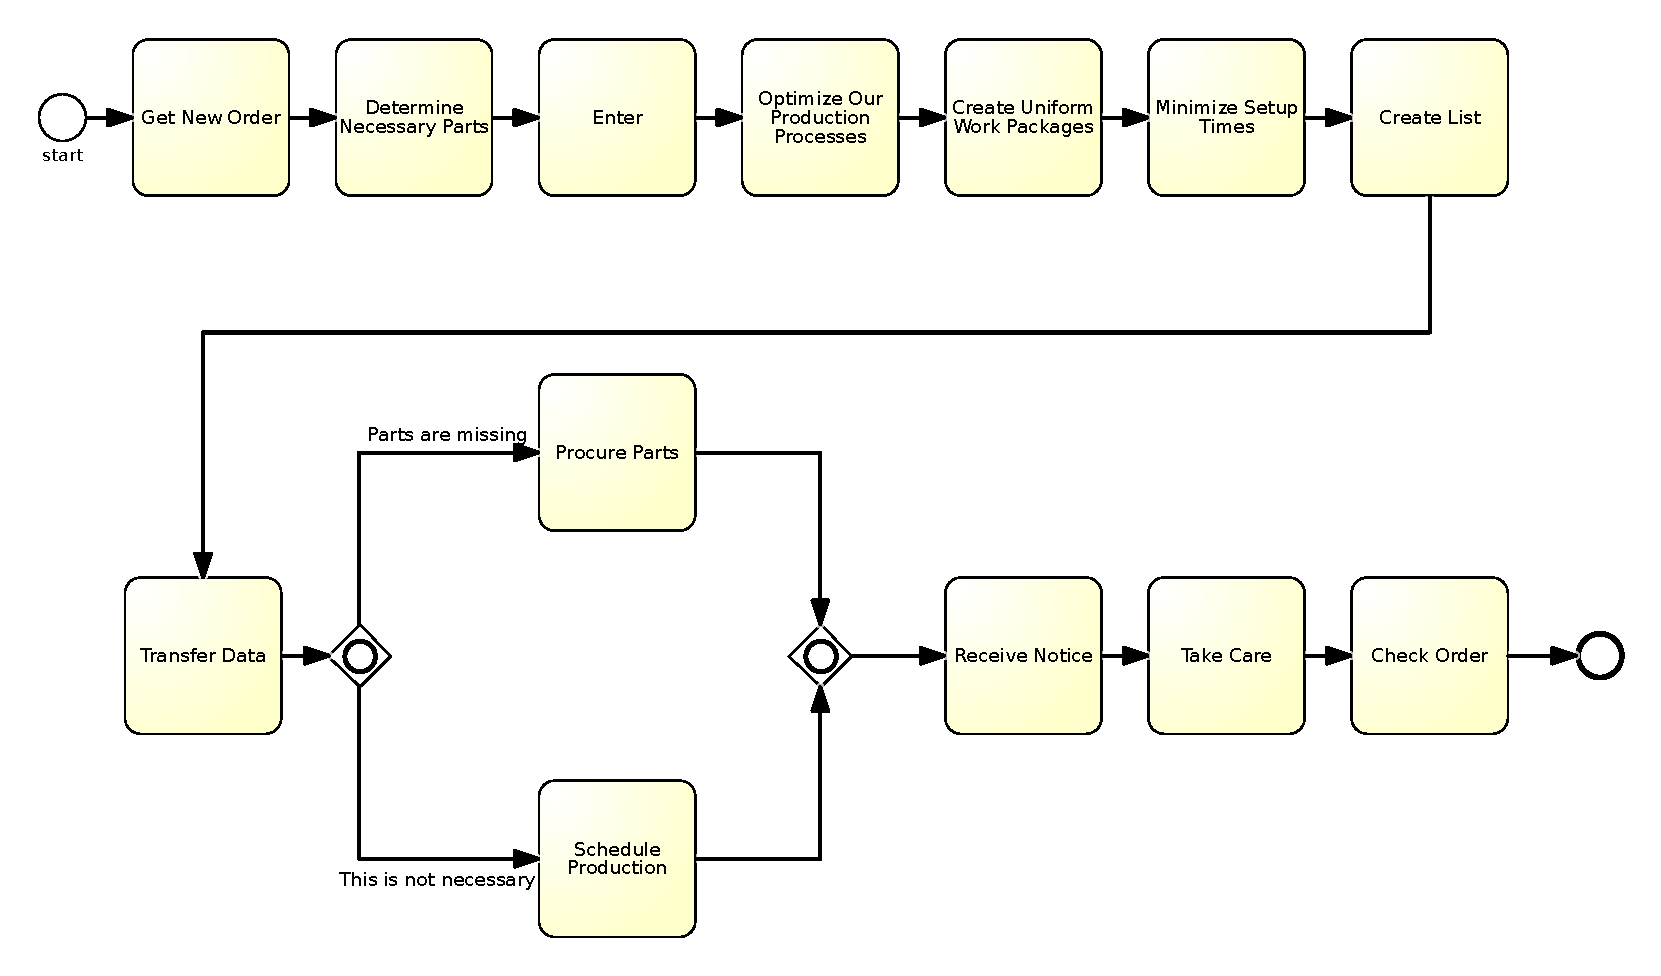
\includegraphics[width=\hsize]{./generated_bpmn/model21.pdf}
	\caption{BPMN diagram for process model 21 generated from spreadsheet-based model}
	\label{bpmn:generated_model21}
\end{figure}

\begin{figure}[H]
	\centering
	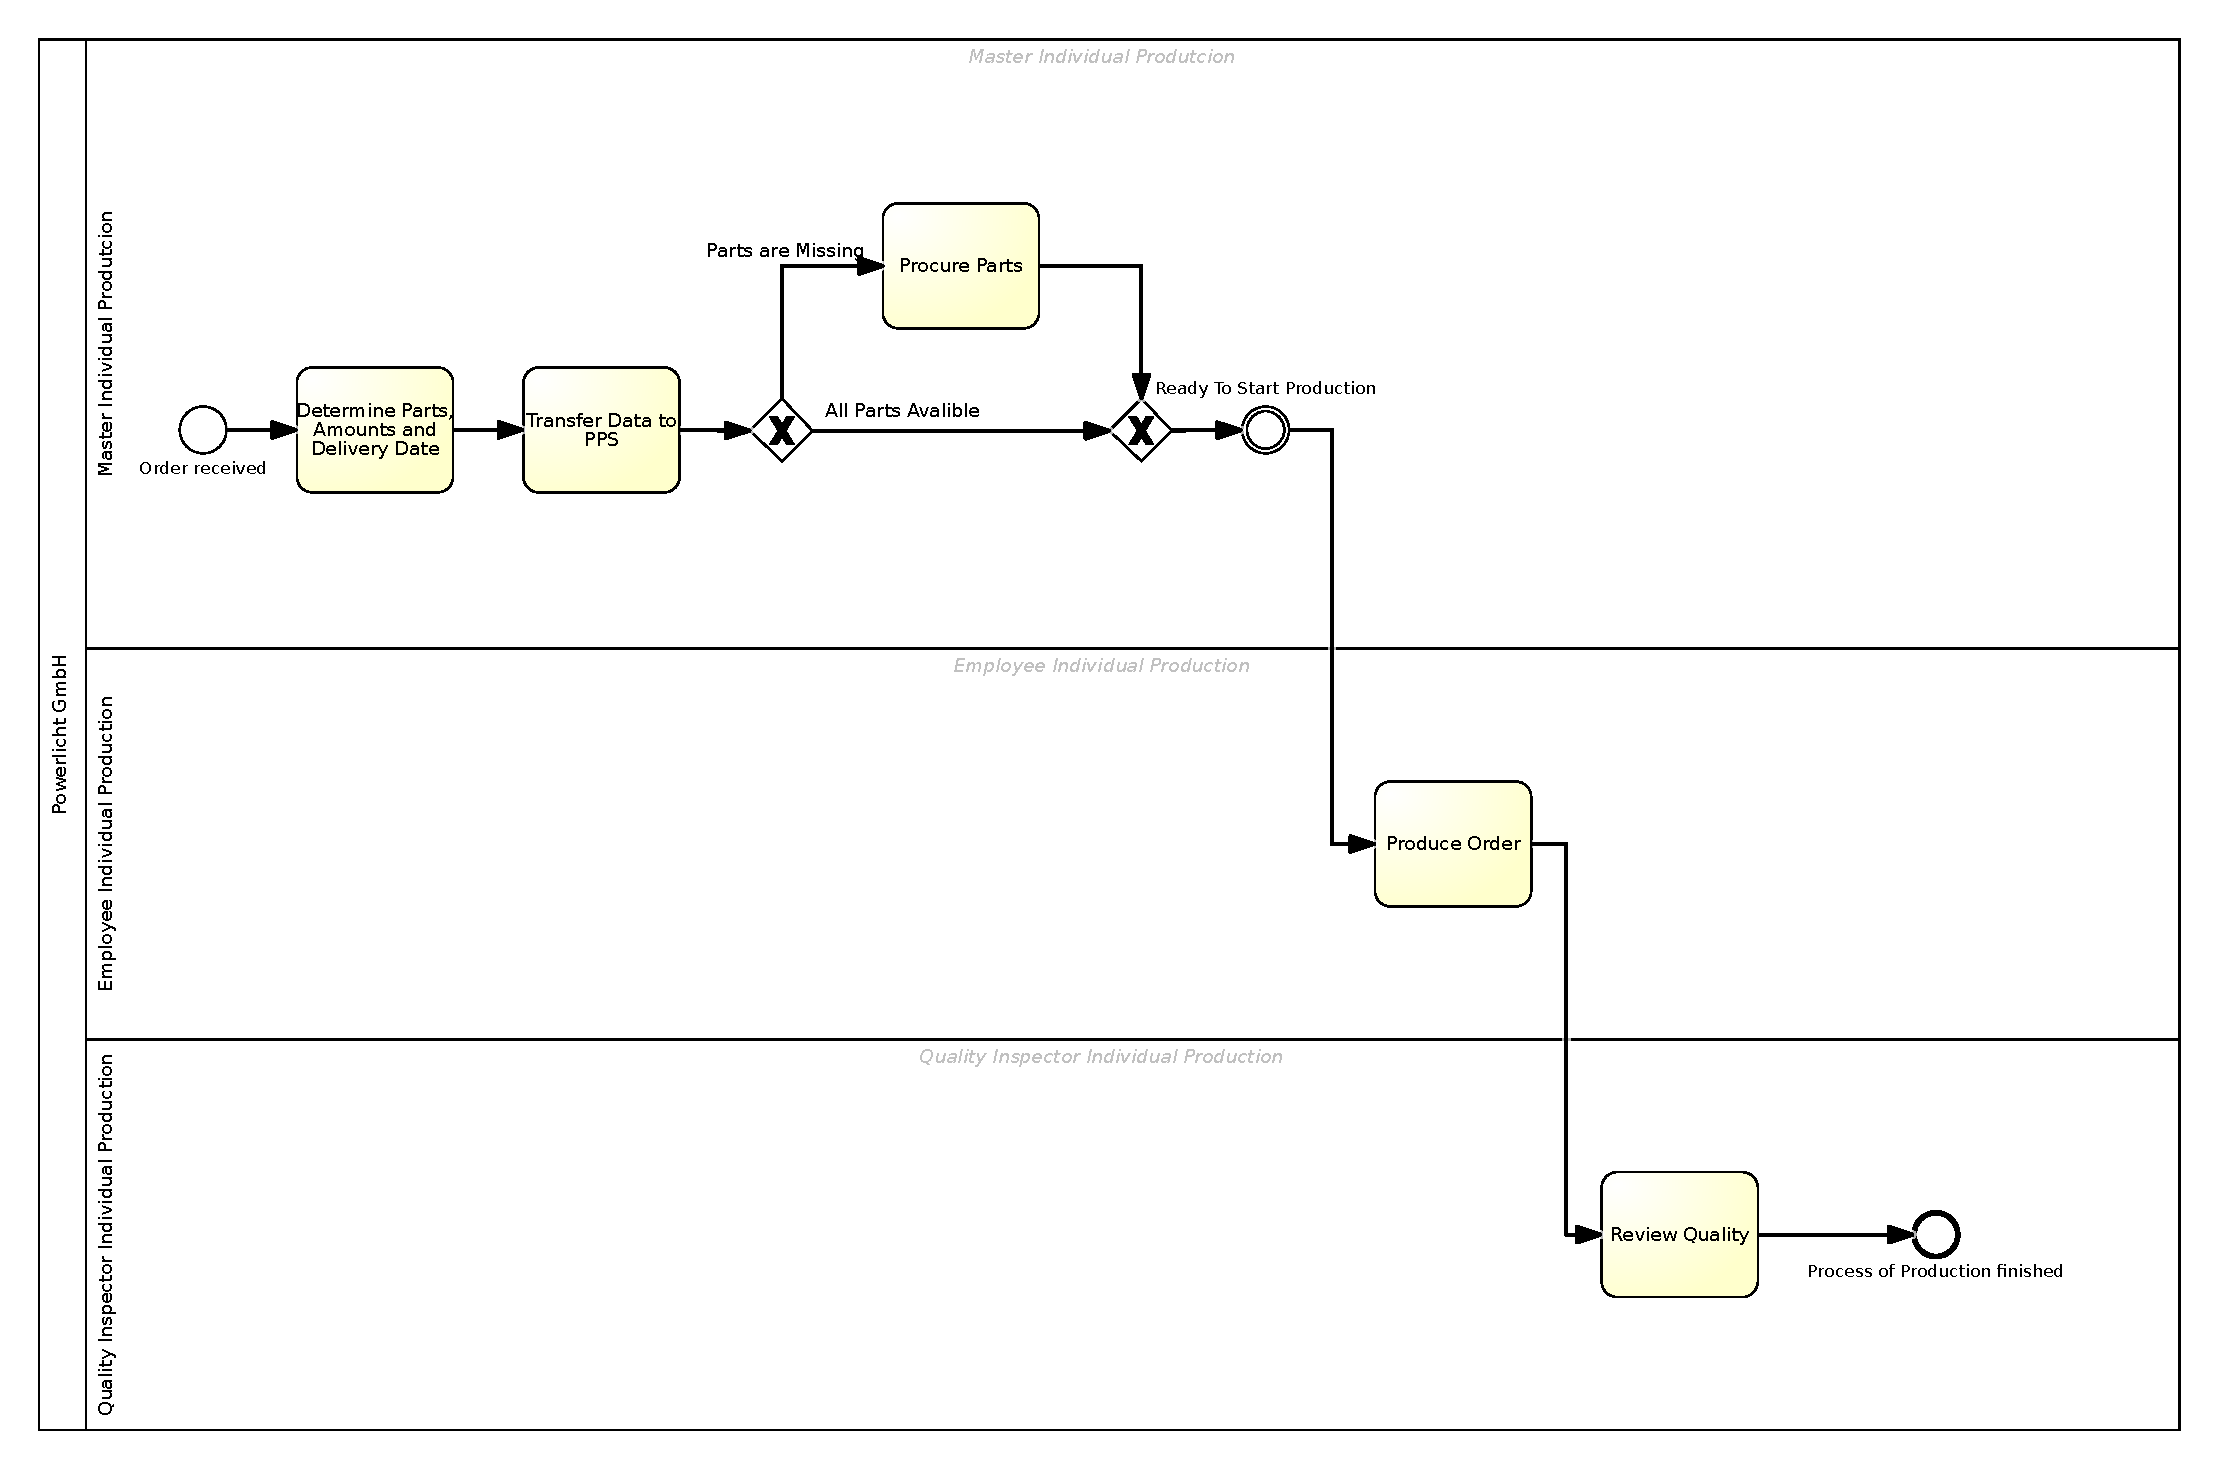
\includegraphics[width=\hsize]{./bpmn/model21.pdf}
	\caption{Hand-made BPMN diagram for process model 21}
	\label{bpmn:model21}
\end{figure}

\section{Model 22}
\begin{tcolorbox}[
	breakable,
	arc=0mm,
	left=1pt,
	right = 1pt,
	boxrule=0mm,
	colback = {white},
	]
	\texttt{\input{./models/model22.txt}}
\end{tcolorbox}
\captionof{textdesc}{Text description for model 22}
\label{txt:model22}

{\scriptsize
	\begin{longtable}{|p{0.03 \hsize}|p{0.25 \hsize}|p{0.15 \hsize}|p{0.2 \hsize}|p{0.1 \hsize}|p{0.1 \hsize}|}
		\hline
		Order & Activity & Condition & Who & Subprocess & Terminated.
		\\\hline\hline
		\csvreader[late after line=\\\hline]
		{./results/model22_intermediate_model.csv}
		{Order=\Order,Activity=\Activity,Condition=\Condition,Who=\Who,Subprocess=\Subprocess,Terminated=\Terminated}
		{\Order & \Activity & \Condition & \Who & \Subprocess & \Terminated}
		\caption{Spreadsheet-based description for process model 22}
		\label{csv:model22}
	\end{longtable}
}

\begin{figure}[H]
	\centering
	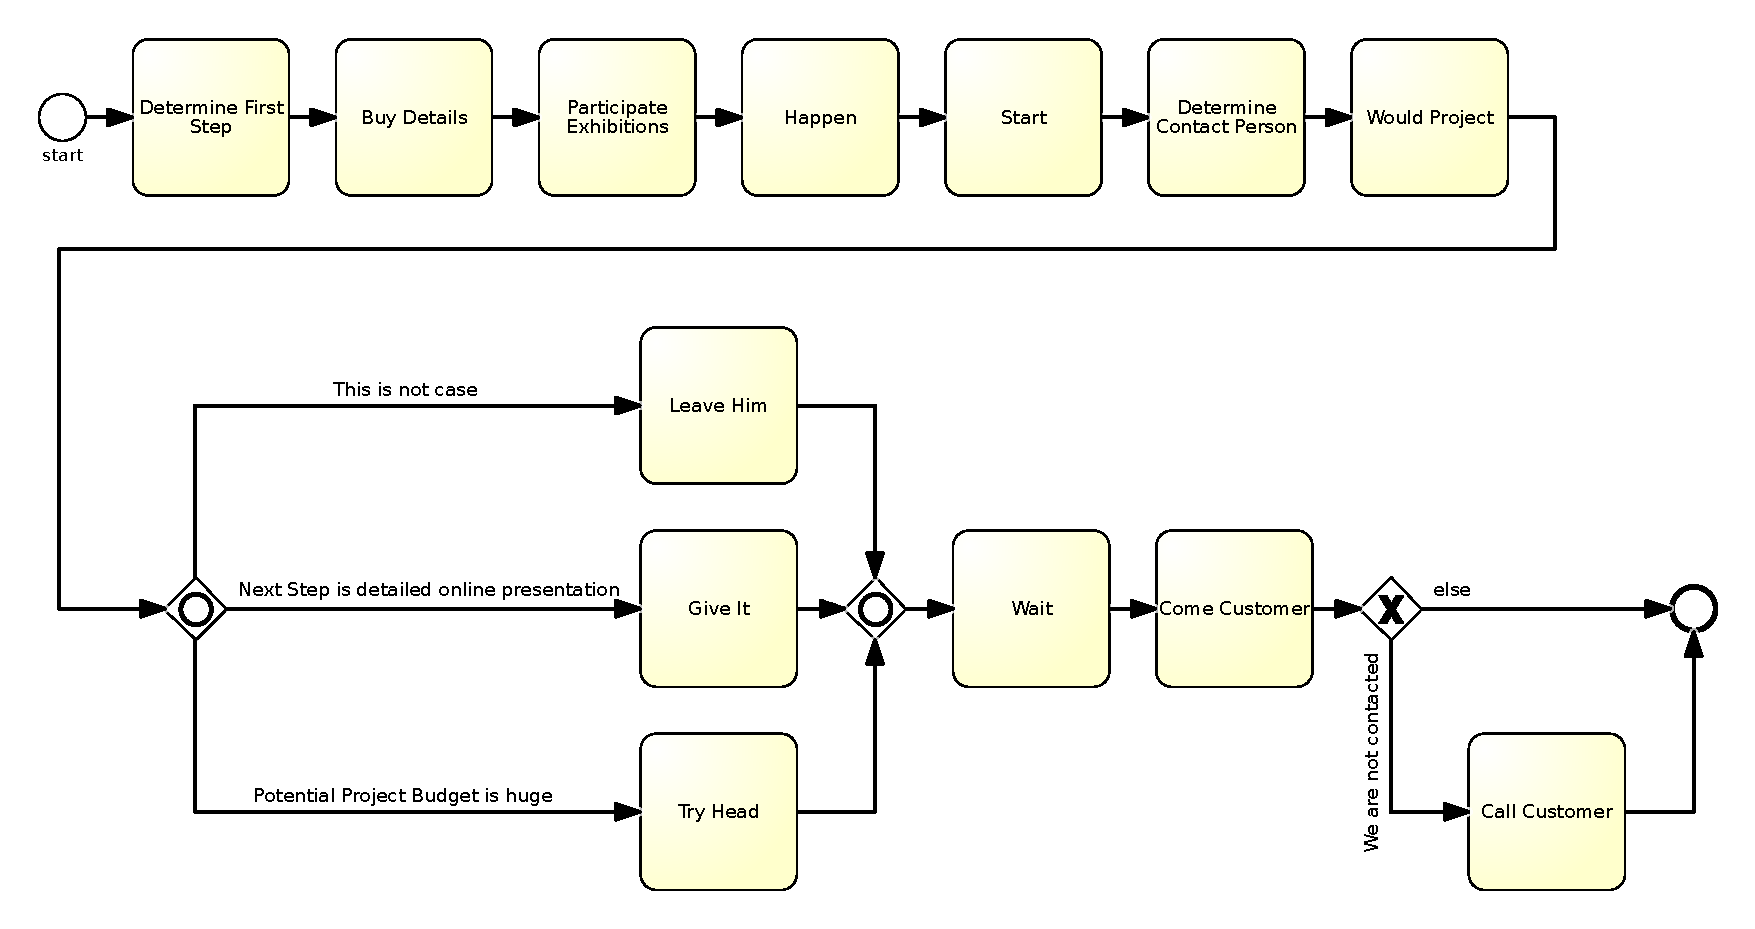
\includegraphics[scale=0.4]{./generated_bpmn/model22.pdf}
	\caption{BPMN diagram for process model 22 generated from spreadsheet-based model}
	\label{bpmn:generated_model22}
\end{figure}

\begin{figure}[H]
	\centering
	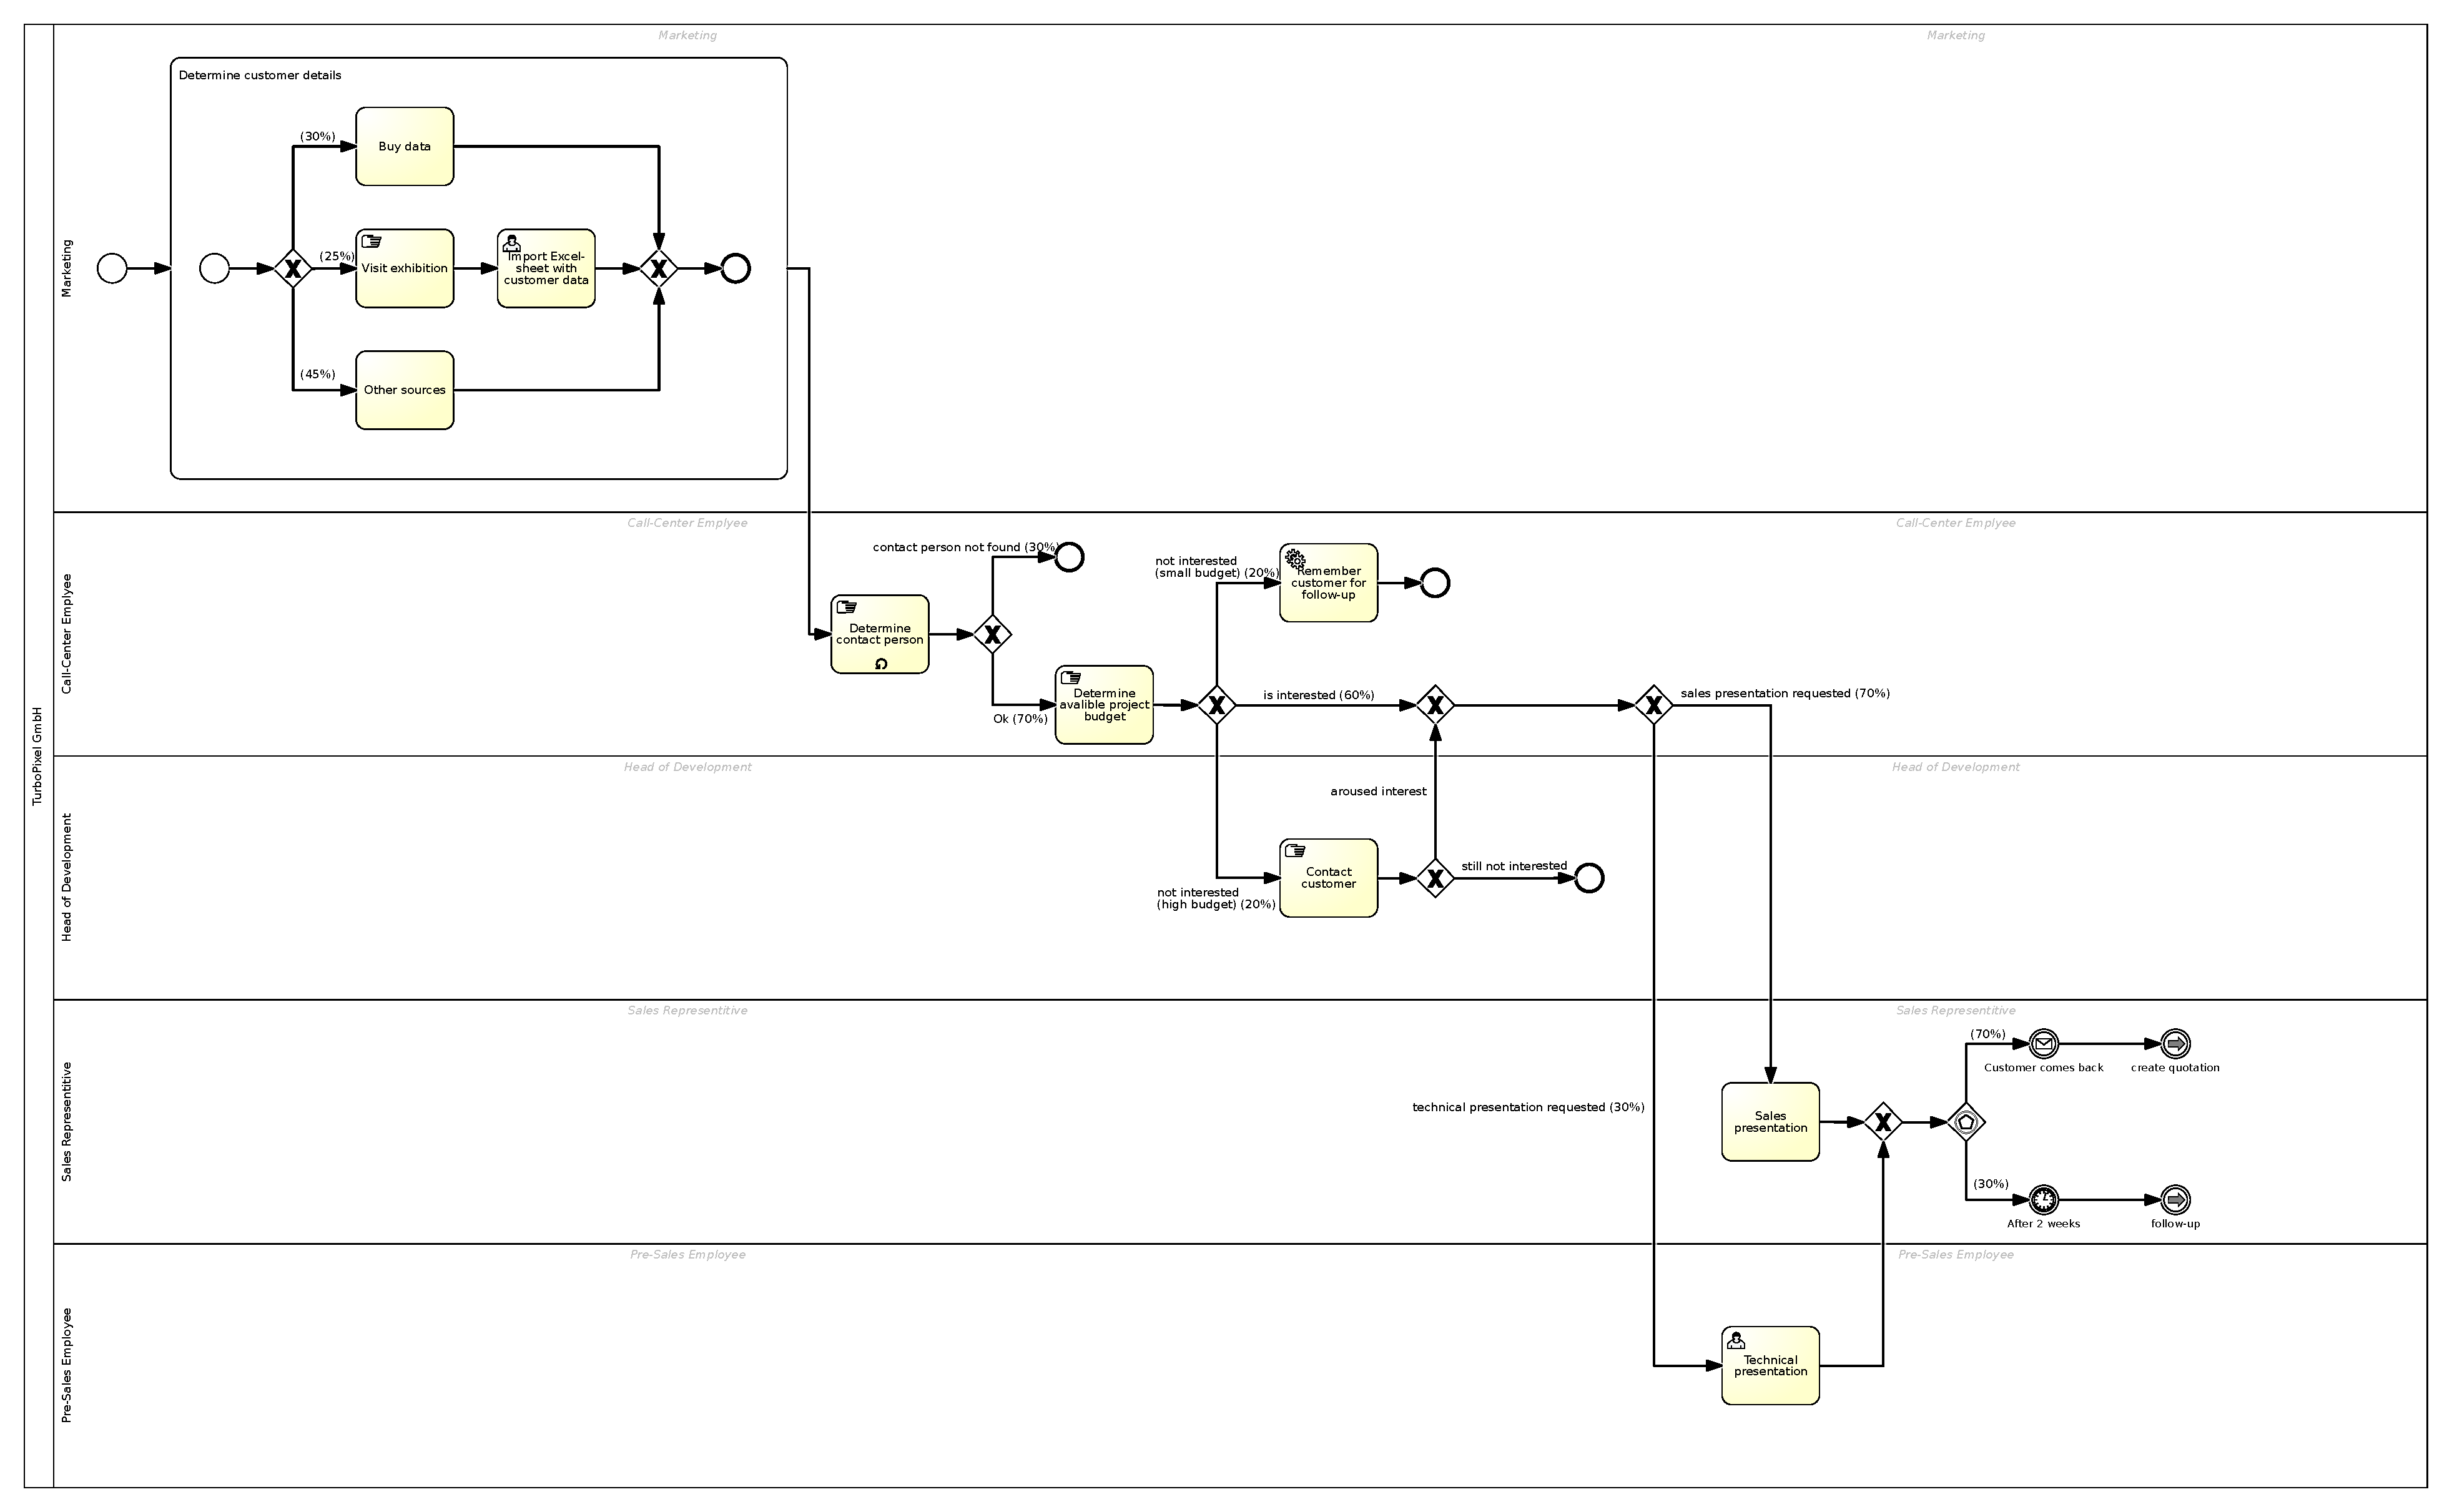
\includegraphics[width=0.95\textheight, angle=90]{./bpmn/model22.pdf}
	\caption{Hand-made BPMN diagram for process model 22}
	\label{bpmn:model22}
\end{figure}

\section{Model 23}
\begin{tcolorbox}[
	breakable,
	arc=0mm,
	left=1pt,
	right = 1pt,
	boxrule=0mm,
	colback = {white},
	]
	\texttt{\input{./models/model23.txt}}
\end{tcolorbox}
\captionof{textdesc}{Text description for model 23}
\label{txt:model23}

{\scriptsize
	\begin{longtable}{|p{0.03 \hsize}|p{0.25 \hsize}|p{0.15 \hsize}|p{0.2 \hsize}|p{0.1 \hsize}|p{0.1 \hsize}|}
		\hline
		Order & Activity & Condition & Who & Subprocess & Terminated.
		\\\hline\hline
		\csvreader[late after line=\\\hline]
		{./results/model23_intermediate_model.csv}
		{Order=\Order,Activity=\Activity,Condition=\Condition,Who=\Who,Subprocess=\Subprocess,Terminated=\Terminated}
		{\Order & \Activity & \Condition & \Who & \Subprocess & \Terminated}
		\caption{Spreadsheet-based description for process model 23}
		\label{csv:model23}
	\end{longtable}
}

\begin{figure}[H]
	\centering
	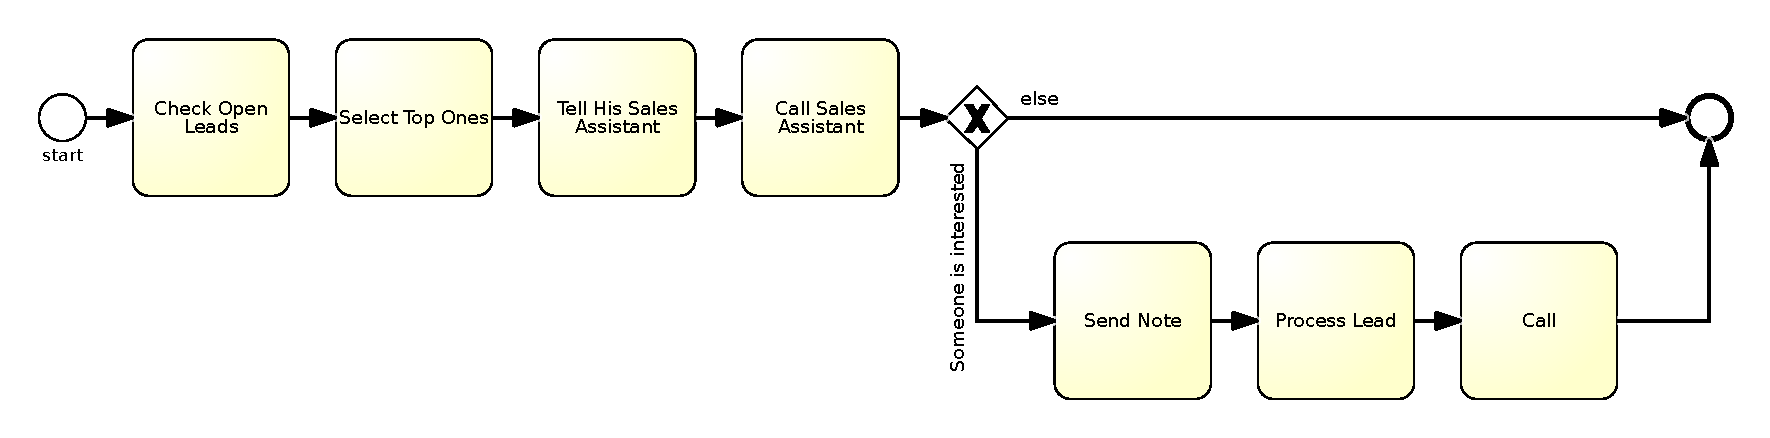
\includegraphics[width=\hsize]{./generated_bpmn/model23.pdf}
	\caption{BPMN diagram for process model 23 generated from spreadsheet-based model}
	\label{bpmn:generated_model23}
\end{figure}

\begin{figure}[H]
	\centering
	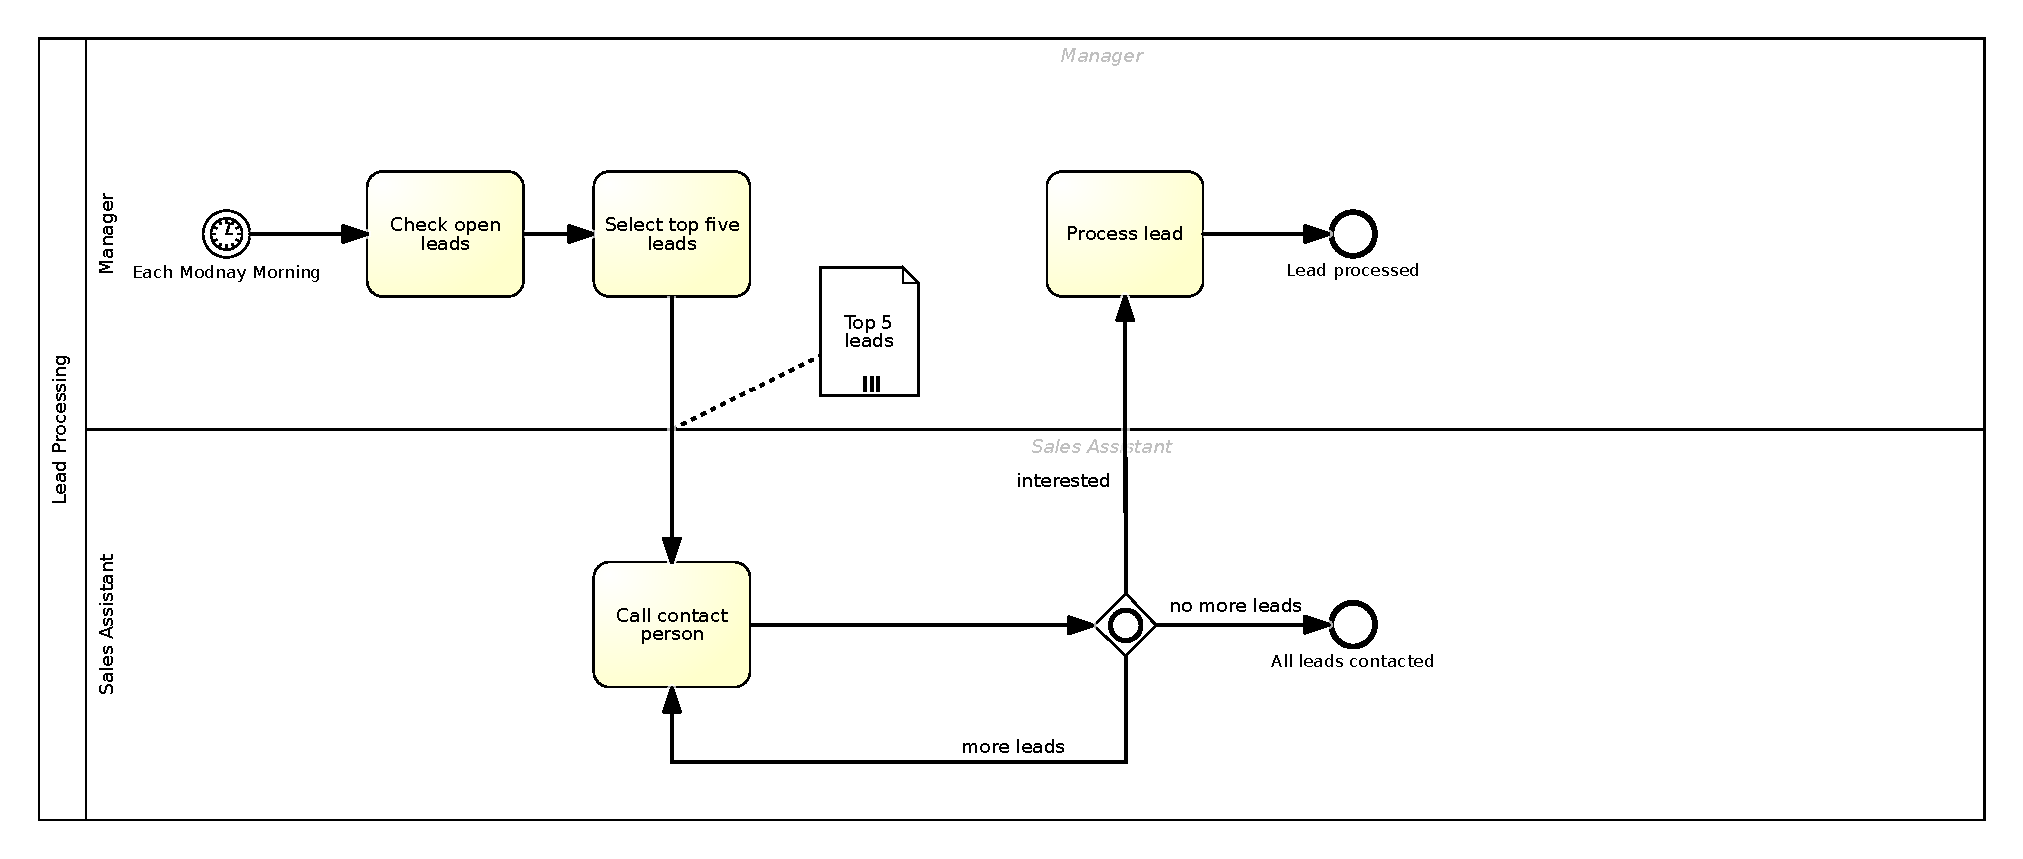
\includegraphics[width=\hsize]{./bpmn/model23.pdf}
	\caption{Hand-made BPMN diagram for process model 23}
	\label{bpmn:model23}
\end{figure}

\section{Model 24}
\begin{tcolorbox}[
	breakable,
	arc=0mm,
	left=1pt,
	right = 1pt,
	boxrule=0mm,
	colback = {white},
	]
	\texttt{\input{./models/model24.txt}}
\end{tcolorbox}
\captionof{textdesc}{Text description for model 24}
\label{txt:model24}

{\scriptsize
	\begin{longtable}{|p{0.03 \hsize}|p{0.25 \hsize}|p{0.15 \hsize}|p{0.2 \hsize}|p{0.1 \hsize}|p{0.1 \hsize}|}
		\hline
		Order & Activity & Condition & Who & Subprocess & Terminated.
		\\\hline\hline
		\csvreader[late after line=\\\hline]
		{./results/model24_intermediate_model.csv}
		{Order=\Order,Activity=\Activity,Condition=\Condition,Who=\Who,Subprocess=\Subprocess,Terminated=\Terminated}
		{\Order & \Activity & \Condition & \Who & \Subprocess & \Terminated}
		\caption{Spreadsheet-based description for process model 24}
		\label{csv:model24}
	\end{longtable}
}

\begin{figure}[H]
	\centering
	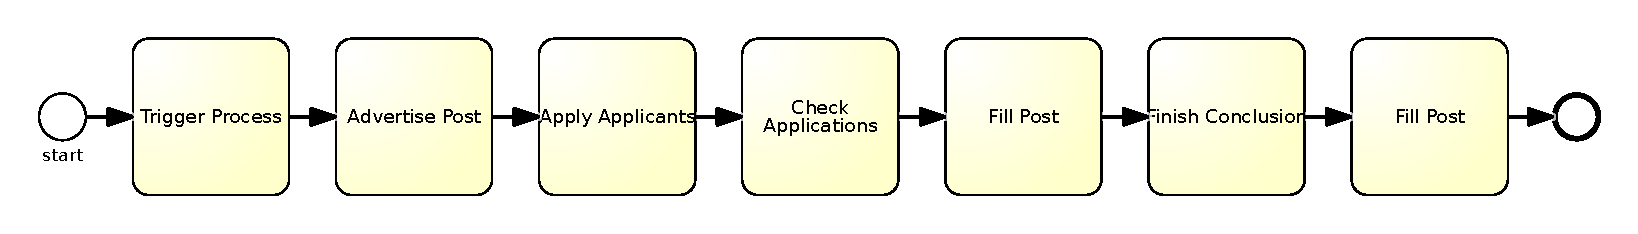
\includegraphics[width=\hsize]{./generated_bpmn/model24.pdf}
	\caption{BPMN diagram for process model 24 generated from spreadsheet-based model}
	\label{bpmn:generated_model24}
\end{figure}

\begin{figure}[H]
	\centering
	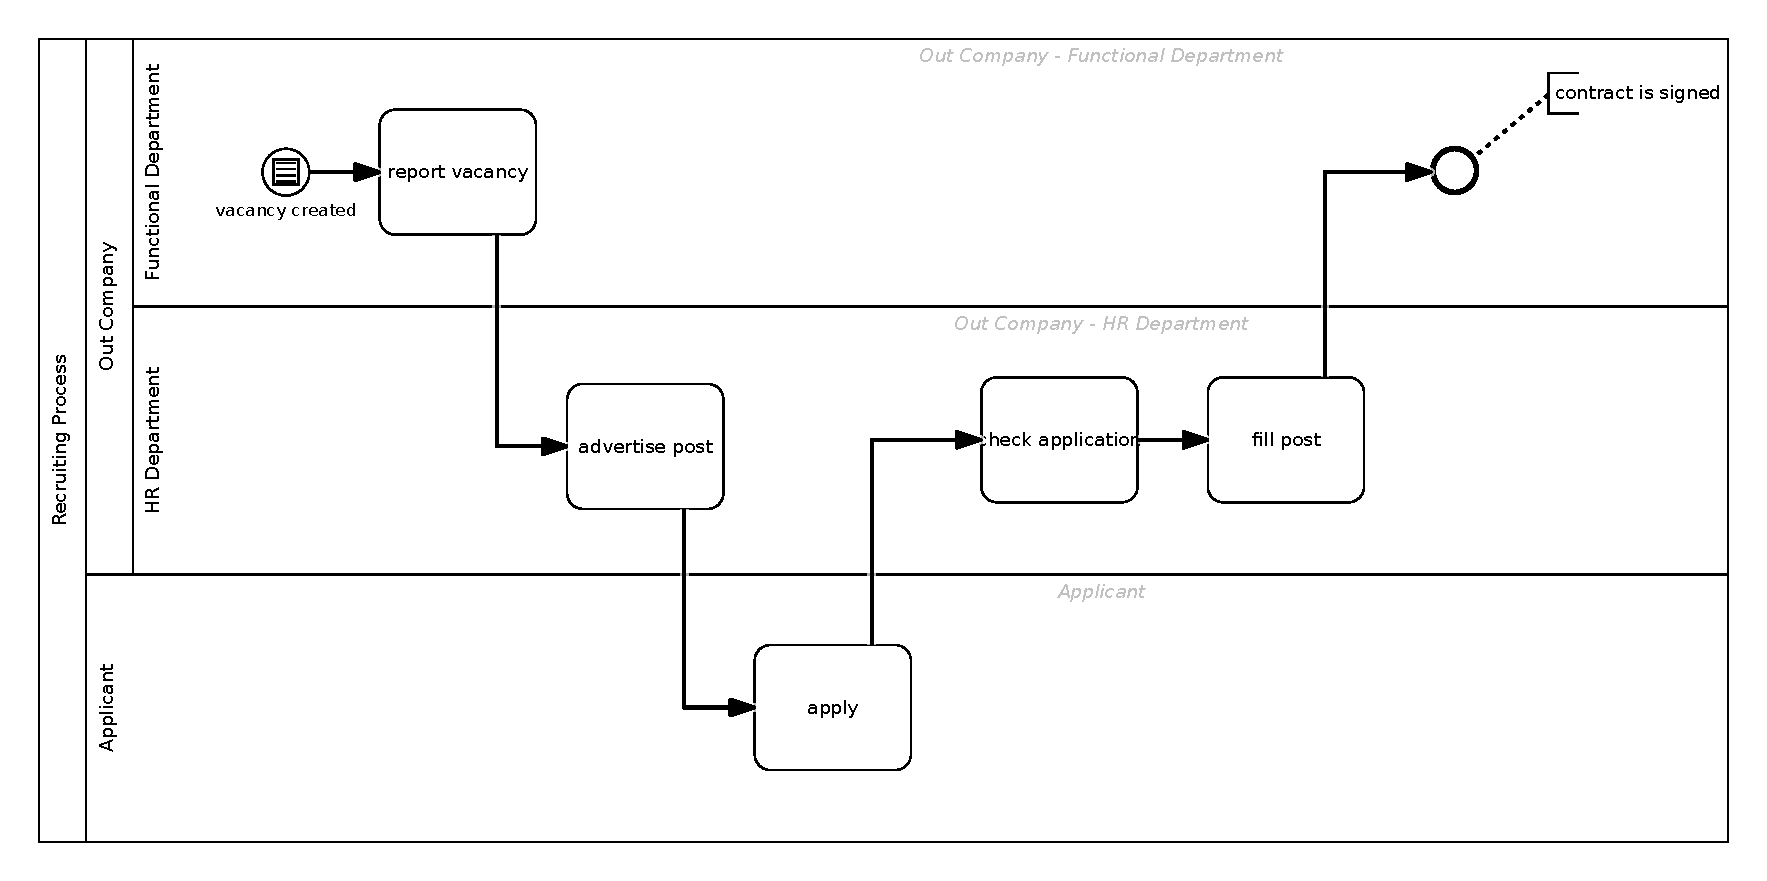
\includegraphics[width=\hsize]{./bpmn/model24.pdf}
	\caption{Hand-made BPMN diagram for process model 24}
	\label{bpmn:model24}
\end{figure}

\section{Model 25}
\begin{tcolorbox}[
	breakable,
	arc=0mm,
	left=1pt,
	right = 1pt,
	boxrule=0mm,
	colback = {white},
	]
	\texttt{\input{./models/model25.txt}}
\end{tcolorbox}
\captionof{textdesc}{Text description for model 25}
\label{txt:model25}
\newpage
{\scriptsize
	\begin{longtable}{|p{0.03 \hsize}|p{0.25 \hsize}|p{0.15 \hsize}|p{0.2 \hsize}|p{0.1 \hsize}|p{0.1 \hsize}|}
		\hline
		Order & Activity & Condition & Who & Subprocess & Terminated.
		\\\hline\hline
		\csvreader[late after line=\\\hline]
		{./results/model25_intermediate_model.csv}
		{Order=\Order,Activity=\Activity,Condition=\Condition,Who=\Who,Subprocess=\Subprocess,Terminated=\Terminated}
		{\Order & \Activity & \Condition & \Who & \Subprocess & \Terminated}
		\caption{Spreadsheet-based description for process model 25}
		\label{csv:model25}
	\end{longtable}
}

\begin{figure}[H]
	\centering
	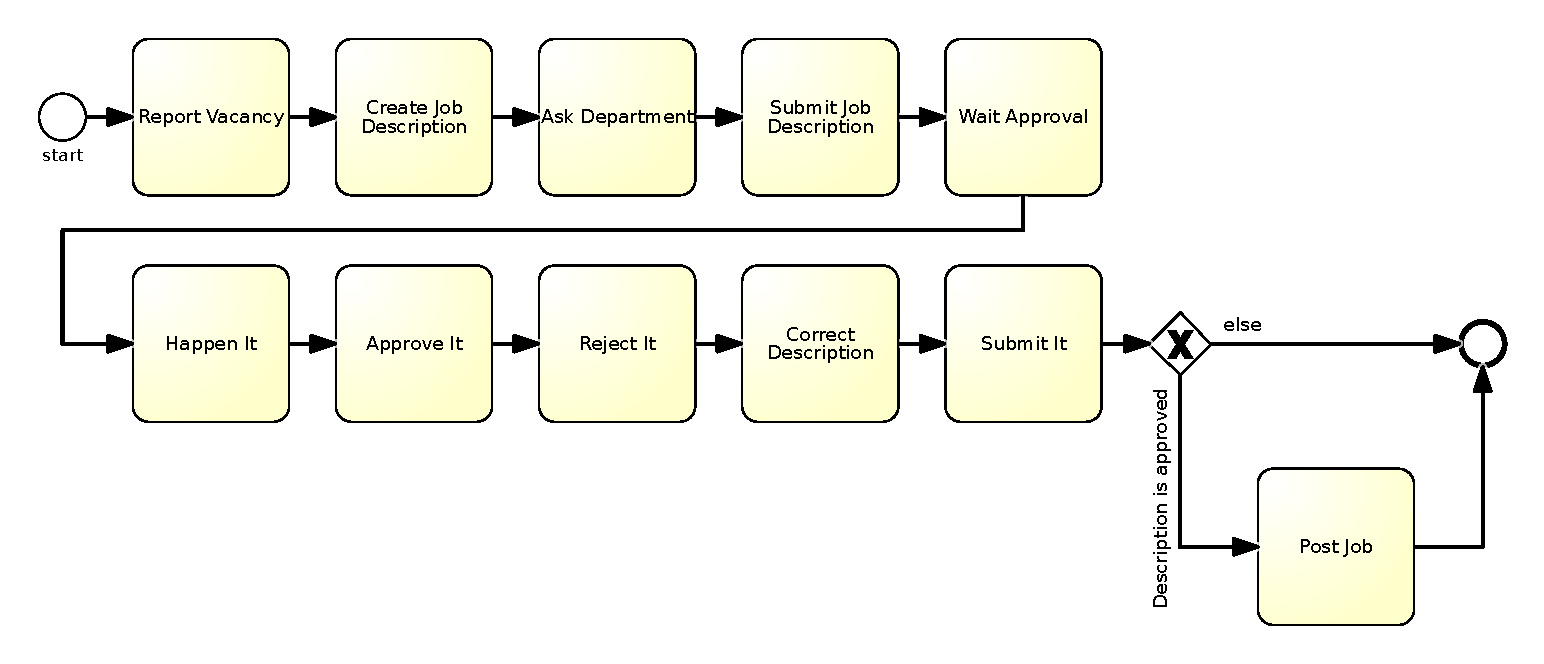
\includegraphics[width=\hsize]{./generated_bpmn/model25.pdf}
	\caption{BPMN diagram for process model 25 generated from spreadsheet-based model}
	\label{bpmn:generated_model25}
\end{figure}

\begin{figure}[H]
	\centering
	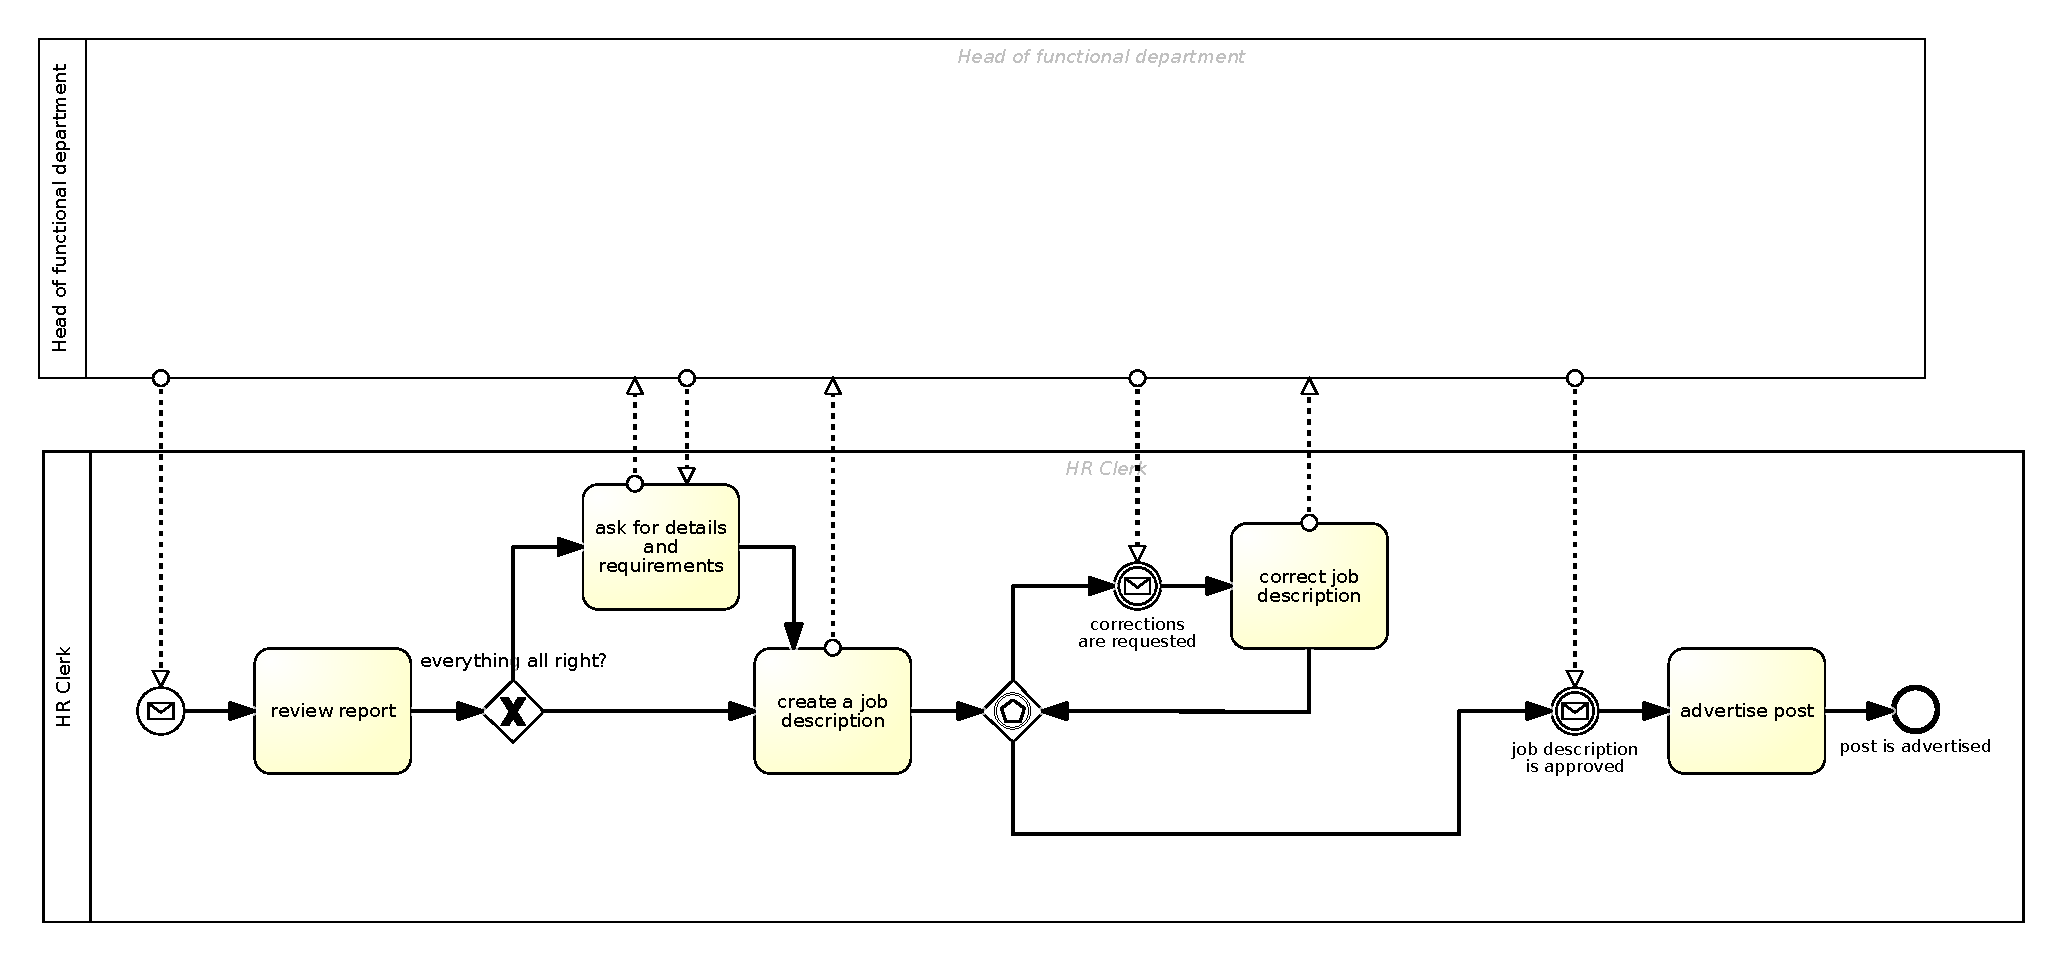
\includegraphics[width=\hsize]{./bpmn/model25.pdf}
	\caption{Hand-made BPMN diagram for process model 25}
	\label{bpmn:model25}
\end{figure}

\section{Model 26}
\begin{tcolorbox}[
	breakable,
	arc=0mm,
	left=1pt,
	right = 1pt,
	boxrule=0mm,
	colback = {white},
	]
	\texttt{\input{./models/model26.txt}}
\end{tcolorbox}
\captionof{textdesc}{Text description for model 26}
\label{txt:model26}

{\scriptsize
	\begin{longtable}{|p{0.03 \hsize}|p{0.25 \hsize}|p{0.15 \hsize}|p{0.2 \hsize}|p{0.1 \hsize}|p{0.1 \hsize}|}
		\hline
		Order & Activity & Condition & Who & Subprocess & Terminated.
		\\\hline\hline
		\csvreader[late after line=\\\hline]
		{./results/model26_intermediate_model.csv}
		{Order=\Order,Activity=\Activity,Condition=\Condition,Who=\Who,Subprocess=\Subprocess,Terminated=\Terminated}
		{\Order & \Activity & \Condition & \Who & \Subprocess & \Terminated}
		\caption{Spreadsheet-based description for process model 26}
		\label{csv:model26}
	\end{longtable}
}

\begin{figure}[H]
	\centering
	\includegraphics[width=\hsize]{./generated_bpmn/model26.pdf}
	\caption{BPMN diagram for process model 26 generated from spreadsheet-based model}
	\label{bpmn:generated_model26}
\end{figure}

\begin{figure}[H]
	\centering
	\includegraphics[width=\hsize]{./bpmn/model26.pdf}
	\caption{Hand-made BPMN diagram for process model 26}
	\label{bpmn:model26}
\end{figure}

\section{Model 27}
\begin{tcolorbox}[
	breakable,
	arc=0mm,
	left=1pt,
	right = 1pt,
	boxrule=0mm,
	colback = {white},
	]
	\texttt{\input{./models/model27.txt}}
\end{tcolorbox}
\captionof{textdesc}{Text description for model 27}
\label{txt:model27}

{\scriptsize
	\begin{longtable}{|p{0.03 \hsize}|p{0.25 \hsize}|p{0.15 \hsize}|p{0.2 \hsize}|p{0.1 \hsize}|p{0.1 \hsize}|}
		\hline
		Order & Activity & Condition & Who & Subprocess & Terminated.
		\\\hline\hline
		\csvreader[late after line=\\\hline]
		{./results/model27_intermediate_model.csv}
		{Order=\Order,Activity=\Activity,Condition=\Condition,Who=\Who,Subprocess=\Subprocess,Terminated=\Terminated}
		{\Order & \Activity & \Condition & \Who & \Subprocess & \Terminated}
		\caption{Spreadsheet-based description for process model 27}
		\label{csv:model27}
	\end{longtable}
}

\begin{figure}[H]
	\centering
	\includegraphics[width=\hsize]{./generated_bpmn/model27.pdf}
	\caption{BPMN diagram for process model 27 generated from spreadsheet-based model}
	\label{bpmn:generated_model27}
\end{figure}

\begin{figure}[H]
	\centering
	\includegraphics[width=\hsize]{./bpmn/model27.pdf}
	\caption{Hand-made BPMN diagram for process model 27}
	\label{bpmn:model27}
\end{figure}

\section{Model 28}
\begin{tcolorbox}[
	breakable,
	arc=0mm,
	left=1pt,
	right = 1pt,
	boxrule=0mm,
	colback = {white},
	]
	\texttt{\input{./models/model28.txt}}
\end{tcolorbox}
\captionof{textdesc}{Text description for model 28}
\label{txt:model28}

{\scriptsize
	\begin{longtable}{|p{0.03 \hsize}|p{0.25 \hsize}|p{0.15 \hsize}|p{0.2 \hsize}|p{0.1 \hsize}|p{0.1 \hsize}|}
		\hline
		Order & Activity & Condition & Who & Subprocess & Terminated.
		\\\hline\hline
		\csvreader[late after line=\\\hline]
		{./results/model28_intermediate_model.csv}
		{Order=\Order,Activity=\Activity,Condition=\Condition,Who=\Who,Subprocess=\Subprocess,Terminated=\Terminated}
		{\Order & \Activity & \Condition & \Who & \Subprocess & \Terminated}
		\caption{Spreadsheet-based description for process model 28}
		\label{csv:model28}
	\end{longtable}
}

\begin{figure}[H]
	\centering
	\includegraphics[width=\hsize]{./generated_bpmn/model28.pdf}
	\caption{BPMN diagram for process model 28 generated from spreadsheet-based model}
	\label{bpmn:generated_model28}
\end{figure}

\begin{figure}[H]
	\centering
	\includegraphics[width=\hsize]{./bpmn/model28.pdf}
	\caption{Hand-made BPMN diagram for process model 28}
	\label{bpmn:model28}
\end{figure}

\section{Model 29}
\begin{tcolorbox}[
	breakable,
	arc=0mm,
	left=1pt,
	right = 1pt,
	boxrule=0mm,
	colback = {white},
	]
	\texttt{\input{./models/model29.txt}}
\end{tcolorbox}
\captionof{textdesc}{Text description for model 29}
\label{txt:model29}

{\scriptsize
	\begin{longtable}{|p{0.03 \hsize}|p{0.25 \hsize}|p{0.15 \hsize}|p{0.2 \hsize}|p{0.1 \hsize}|p{0.1 \hsize}|}
		\hline
		Order & Activity & Condition & Who & Subprocess & Terminated.
		\\\hline\hline
		\csvreader[late after line=\\\hline]
		{./results/model29_intermediate_model.csv}
		{Order=\Order,Activity=\Activity,Condition=\Condition,Who=\Who,Subprocess=\Subprocess,Terminated=\Terminated}
		{\Order & \Activity & \Condition & \Who & \Subprocess & \Terminated}
		\caption{Spreadsheet-based description for process model 29}
		\label{csv:model29}
	\end{longtable}
}

\begin{figure}[H]
	\centering
	\includegraphics[width=\hsize]{./generated_bpmn/model29.pdf}
	\caption{BPMN diagram for process model 29 generated from spreadsheet-based model}
	\label{bpmn:generated_model29}
\end{figure}

\begin{figure}[H]
	\centering
	\includegraphics[width=\hsize]{./bpmn/model29.pdf}
	\caption{Hand-made BPMN diagram for process model 29}
	\label{bpmn:model29}
\end{figure}

\section{Model 30}
\begin{tcolorbox}[
	breakable,
	arc=0mm,
	left=1pt,
	right = 1pt,
	boxrule=0mm,
	colback = {white},
	]
	\texttt{\input{./models/model30.txt}}
\end{tcolorbox}
\captionof{textdesc}{Text description for model 30}
\label{txt:model30}

{\scriptsize
	\begin{longtable}{|p{0.03 \hsize}|p{0.25 \hsize}|p{0.15 \hsize}|p{0.2 \hsize}|p{0.1 \hsize}|p{0.1 \hsize}|}
		\hline
		Order & Activity & Condition & Who & Subprocess & Terminated.
		\\\hline\hline
		\csvreader[late after line=\\\hline]
		{./results/model30_intermediate_model.csv}
		{Order=\Order,Activity=\Activity,Condition=\Condition,Who=\Who,Subprocess=\Subprocess,Terminated=\Terminated}
		{\Order & \Activity & \Condition & \Who & \Subprocess & \Terminated}
		\caption{Spreadsheet-based description for process model 30}
		\label{csv:model30}
	\end{longtable}
}

\begin{figure}[H]
	\centering
	\includegraphics[width=\hsize]{./generated_bpmn/model30.pdf}
	\caption{BPMN diagram for process model 30 generated from spreadsheet-based model}
	\label{bpmn:generated_model30}
\end{figure}

\begin{figure}[H]
	\centering
	\includegraphics[width=\hsize]{./bpmn/model30.pdf}
	\caption{Hand-made BPMN diagram for process model 30}
	\label{bpmn:model30}
\end{figure}

\section{Model 31}
\begin{tcolorbox}[
	breakable,
	arc=0mm,
	left=1pt,
	right = 1pt,
	boxrule=0mm,
	colback = {white},
	]
	\texttt{\input{./models/model31.txt}}
\end{tcolorbox}
\captionof{textdesc}{Text description for model 31}
\label{txt:model31}

{\scriptsize
	\begin{longtable}{|p{0.03 \hsize}|p{0.25 \hsize}|p{0.15 \hsize}|p{0.2 \hsize}|p{0.1 \hsize}|p{0.1 \hsize}|}
		\hline
		Order & Activity & Condition & Who & Subprocess & Terminated.
		\\\hline\hline
		\csvreader[late after line=\\\hline]
		{./results/model31_intermediate_model.csv}
		{Order=\Order,Activity=\Activity,Condition=\Condition,Who=\Who,Subprocess=\Subprocess,Terminated=\Terminated}
		{\Order & \Activity & \Condition & \Who & \Subprocess & \Terminated}
		\caption{Spreadsheet-based description for process model 31}
		\label{csv:model31}
	\end{longtable}
}

\begin{figure}[H]
	\centering
	\includegraphics[width=\hsize]{./generated_bpmn/model31.pdf}
	\caption{BPMN diagram for process model 31 generated from spreadsheet-based model}
	\label{bpmn:generated_model31}
\end{figure}

\begin{figure}[H]
	\centering
	\includegraphics[width=\hsize]{./bpmn/model31.pdf}
	\caption{Hand-made BPMN diagram for process model 31}
	\label{bpmn:model31}
\end{figure}

\section{Model 32}
\begin{tcolorbox}[
	breakable,
	arc=0mm,
	left=1pt,
	right = 1pt,
	boxrule=0mm,
	colback = {white},
	]
	\texttt{\input{./models/model32.txt}}
\end{tcolorbox}
\captionof{textdesc}{Text description for model 32}
\label{txt:model32}

{\scriptsize
	\begin{longtable}{|p{0.03 \hsize}|p{0.25 \hsize}|p{0.15 \hsize}|p{0.2 \hsize}|p{0.1 \hsize}|p{0.1 \hsize}|}
		\hline
		Order & Activity & Condition & Who & Subprocess & Terminated.
		\\\hline\hline
		\csvreader[late after line=\\\hline]
		{./results/model32_intermediate_model.csv}
		{Order=\Order,Activity=\Activity,Condition=\Condition,Who=\Who,Subprocess=\Subprocess,Terminated=\Terminated}
		{\Order & \Activity & \Condition & \Who & \Subprocess & \Terminated}
		\caption{Spreadsheet-based description for process model 32}
		\label{csv:model32}
	\end{longtable}
}

\begin{figure}[H]
	\centering
	\includegraphics[width=\hsize]{./generated_bpmn/model32.pdf}
	\caption{BPMN diagram for process model 32 generated from spreadsheet-based model}
	\label{bpmn:generated_model32}
\end{figure}

\begin{figure}[H]
	\centering
	\includegraphics[width=0.95\textheight, angle=90]{./bpmn/model32.pdf}
	\caption{Hand-made BPMN diagram for process model 32}
	\label{bpmn:model32}
\end{figure}